\PassOptionsToPackage{table}{xcolor}
\documentclass[11pt,twoside,openright,a4paper]{book}

\usepackage{etoolbox}
\newtoggle{finalversion}
\newtoggle{printing}

\toggletrue{finalversion}
\toggletrue{printing}

\iftoggle{finalversion}{%
  \usepackage[inner=2.5cm, outer=3.5cm, top=3.5cm, bottom=2.5cm, headsep=0.9cm]{geometry}
  % for ADUM cover...
  \usepackage{pdfpages}
}{%
  % NOTE: for reviewing only, easier to read in digital version...
  % same odd/even margins
  \usepackage[inner=3cm, outer=3cm, top=3.5cm, bottom=2.5cm, headsep=0.9cm]{geometry}
}

\usepackage[utf8]{inputenc}
\usepackage[T1]{fontenc}

\usepackage[numbers,sort]{natbib}
\usepackage[french,main=english]{babel}
\usepackage{caption}
\usepackage{listings}


\colorlet{punct}{red!60!black}
\definecolor{background}{HTML}{EEEEEE}
\definecolor{delim}{RGB}{20,105,176}
\colorlet{numb}{magenta!60!black}

\lstdefinelanguage{json}{
    basicstyle=\scriptsize\ttfamily,
    numbers=left,
    numberstyle=\scriptsize,
    stepnumber=1,
    numbersep=8pt,
    showstringspaces=false,
    breaklines=true,
    frame=lines,
    backgroundcolor=\color{background},
    literate=
     *{0}{{{\color{numb}0}}}{1}
      {1}{{{\color{numb}1}}}{1}
      {2}{{{\color{numb}2}}}{1}
      {3}{{{\color{numb}3}}}{1}
      {4}{{{\color{numb}4}}}{1}
      {5}{{{\color{numb}5}}}{1}
      {6}{{{\color{numb}6}}}{1}
      {7}{{{\color{numb}7}}}{1}
      {8}{{{\color{numb}8}}}{1}
      {9}{{{\color{numb}9}}}{1}
      {:}{{{\color{punct}{:}}}}{1}
      {,}{{{\color{punct}{,}}}}{1}
      {\{}{{{\color{delim}{\{}}}}{1}
      {\}}{{{\color{delim}{\}}}}}{1}
      {[}{{{\color{delim}{[}}}}{1}
      {]}{{{\color{delim}{]}}}}{1},
}


\captionsetup[table]{skip=10pt}
% stuff for citation and references...
%\usepackage[isbn=false,doi=true,url=false,natbib=true,backend=biber]{biblatex} % backref=true
% to have the bibliography in the toc
\usepackage[nottoc,notlot,notlof]{tocbibind}
% for the publications references...
\usepackage{bibentry}

\usepackage{fancyhdr}

\usepackage{afterpage}
\usepackage{pdflscape}
\usepackage[ruled,vlined]{algorithm2e}
\usepackage{gensymb}

% acronym management, based on http://blog.dorian-depriester.fr/latex/latex-specifiez-vos-acronymes-une-bonne-fois-pour-toute
% need to be loaded before hyperref to prevent awful hyperlinks...
\usepackage[xindy,acronyms,nomain,nonumberlist]{glossaries}	% Ensures that all acronyms are defined once
	\let\oldnewacronym\newacronym
	\newcommand*{\provideacronym}[3]{%
	  \ifglsentryexists{#1}{%
	  }{%
	    \oldnewacronym{#1}{#2}{#3}%
	  }%
	}
\makeglossaries

% For TODO management...
% NOTE: todonotes have in fact an option 'disable' for doing the same (but better)...
\iftoggle{finalversion}{%
  \def\todonotestoggle{disable}
  %\newcommand{\todo}[3][nop]{#3}
}{
  \def\todonotestoggle{}
  % see 1.6.5 of todonotes documentation
  \setlength{\marginparwidth}{2.5cm}
}
\usepackage[\todonotestoggle]{todonotes}
\newcommand{\tdi}[2][]{\todo[inline,caption={yatodo},#1]{\begin{minipage}{\textwidth-4pt}#2\end{minipage}}{}}

% (from Ines) permet de faire une table des matieres par chapitre
\usepackage{minitoc}
\setcounter{minitocdepth}{1}

\iftoggle{printing}{
  % we still want hyperref (no PDF-X...) but without the colors!
  \usepackage{hyperref}
  \hypersetup{hidelinks, breaklinks=true}
}{%
  \usepackage{hyperref}
  \hypersetup{urlcolor=blue,linkcolor=blue,citecolor=blue,colorlinks=true,breaklinks=true}
}

% Note: should be loaded *after* hyperref...
\usepackage[french,english]{cleveref}
\crefname{algocf}{alg.}{algs.}
\Crefname{algocf}{Algorithm}{Algorithms}
% for our floating environment...
\crefalias{lstfloat}{listing}

\usepackage{pdflscape}
% Toulouse PhD frontpage
\usepackage[ED=MITT-MITT, Ets=INP]{tlsflyleaf}

\newacronym[longplural={renewable energy sources}]{res}{RES}{renewable energy source}
\newacronym{ghg}{GHG}{greenhouse gas}
\newacronym{milp}{MILP}{Mixed-Integer Linear Programming}
\newacronym{dpm}{DPM}{Dynamic Power Management}
\newacronym{dvfs}{DVFS}{Dynamic Voltage and Frequency Scaling}
\newacronym{qos}{QoS}{Quality of Service}
\newacronym{hpc}{HPC}{High Performance Computing}
\newacronym{ndc}{NDC}{Nationally Determined Contribution}



% ==================
% Setup basic string
% - PhD Title
% - author
% - defence date
% - laboratory
% - cotutelle
\title{\textbf{\large On-line scheduling for IT tasks and power source commitment in datacenters only operated with renewable energy}}
\author{Igor FONTANA DE NARDIN}
\defencedate{31/01/2023}
\lab{Laplace (UMR 5213) et IRIT (UMR 5505)}
%\cotutelle{Nom de l'\'etablissement}

% ==================
% Setup people like your boss, the jury team and the referees
% - First you need to define how number they will be in each category
%   It is done with the commands \nboss{n}, \nreferee{n} and \njudge{n}.
%   You can define more people in each category than the number given 
%   but only the first "\npeople" will be print.
% - Then use the command \makesomeone{<category>}{<number>}{<name>}{<status>}{<other>}
%   where:
%     <category> should be selected in ['boss', 'referee', 'judge']
%     <number>   is the rank for printing the person. 
%                Only number <= "\npeople" will be printed
%     <name>     First name and last name of the people
%     <status>   Is (s)he a "charg\'e de recher" ou un "professeur d'universit\'e"...
%     <other>    Whatever string you want to add (laboratory, jury member place...).
%% Boss
\nboss{2}
\makesomeone{boss}{2}{Stéphane CAUX}{}{}  % Sera affiche en second
\makesomeone{boss}{1}{Patricia STOLF}{}{} % Sera afiche en premier
%% Referee
\nreferee{2}
\makesomeone{referee}{1}{Premier RAPPORTEUR}{}{}
\makesomeone{referee}{2}{Second RAPPORTEUR}{}{}
%% Judges
\njudge{5}
\makesomeone{judge}{1}{Premier MEMBRE}{Professeur d'Université}{Rapporteur}
\makesomeone{judge}{2}{Second MEMBRE}{Professeur d'Université}{Rapporteur}
\makesomeone{judge}{3}{Troisième MEMBRE}{Professeur d'Université}{Examinateur}
\makesomeone{judge}{4}{Quatrième MEMBRE}{Professeur d'Université}{Examinateur}
\makesomeone{judge}{5}{Cinquième MEMBRE}{Professeur d'Université}{Examinateur}

\graphicspath{{Images/}}

% \newcommand\blankpage{%
%     \null
%     \thispagestyle{empty}%
%     \addtocounter{page}{-1}%
%     \newpage}

% ============================================================
% DOCUMENT
\begin{document}
    \pagestyle{plain}
    \makeflyleaf

    \pagestyle{empty}

    \frontmatter

    \dominitoc

    % NOTE fancy page settings (c.f. Inès)
    \renewcommand{\chaptermark}[1]{\markboth {\thechapter.\ #1}{\thechapter.\ #1}}
    \renewcommand{\sectionmark}[1]{ \markright{\thesection. \ #1}}
    \pagestyle{fancy}
    \renewcommand{\headrulewidth}{1pt}
    \fancyhead[RE,LO]{} %\thepage ? 
    \fancyhead[LE]{\nouppercase{\small\rightmark}}
    \fancyhead[RO]{\nouppercase{\small\leftmark}}
    \fancyhead[C]{}  

    \iftoggle{finalversion}{%
    \chapter*{Acknowledgments}
    \chapter*{Acknowledgments}
    }%
    { % NOTE: no ACK in draft and co...
    }

    \chapter{Abstract}
    \label{cha:abstract_english}
    Global warming is one of the biggest humanity challenges. Fossil fuels are one of the world's main sources of energy production, which emits greenhouse gas emissions (GHG) in the atmosphere. This gas creates a barrier in the atmosphere, not allowing heat dissipation in the space. Therefore, Earth's temperature increases, unbalancing our environment. Paris Agreement established some objectives for the end of Century 21. The main goal is to limit the temperature increase to 2 \degree C, trying to limit it to 1.5 \degree C. However, recent reports show we are walking toward a temperature increase of 2.8 \degree C. High temperatures lead to climate and health problems. Different sectors are rethinking their processes and proposing solutions to the global warming problem. The data center sector is a significant GHG emitter, with 1\% of the global energy-related GHG emissions. A way to reduce the data center's impact on GHG emissions is by reducing the energy needed by the servers. However, some authors pointed out a reduction in the processor energy improvements. Furthermore, with the expected increase in Internet users (up to 5.3 billion in 2023), the situation tends to get even worse. 

A possible solution is migrating energy production from brown sources (fossil fuels) to green sources (renewable energy sources - RES). It generates energy from natural sources, such as solar and wind. The biggest drawback of implementing RES is its intermittence since its production comes from nature, depending on the climate conditions. Big cloud providers invest in off-site solar and wind power plants, which means they provide renewable energy to the grid with the same amount they expend. Therefore, they transfer the intermittence problem to third parties. The Datazero2 project proposes a renewable-only data center with only on-site renewable production. This kind of data center would drastically reduce their GHG emissions. However, a renewable-only data center introduces several challenges. We deal with these challenges in two parts: offline and online. The offline side uses predictions to plan short-term decisions but considers the long-term. The online side must apply the offline plan, reacting to the actual events of the data center. Since the predictions are imperfect, the online must find ways to adapt the offline plan, reducing the impact on the user's jobs. Considering these elements, this thesis proposes some approaches to mix offline and online decisions, dealing with the uncertainty coming from renewable production and workload demand.

First, we propose four policies for energy compensation. The main objective of these policies is to adapt the offline plan to approximate the storage levels to the planned levels at the end of a time window. These adaptations are necessary since power production and demand can vary. We demonstrate the impact of respecting the storage levels on the Quality of Service (QoS). After that, we introduce Reinforcement Learning algorithms in the compensation problem, trying to improve the QoS of our policies. More specifically, we use these algorithms to define how to compensate for different scenarios, aiming to increase the number of finished jobs. Therefore, we could still respect the energy storage levels and improve the QoS. Finally, our last contribution is a heuristic that mixes both power and scheduling decisions, seeking to reduce the number of killed jobs and wasted energy. This heuristic is named \emph{\systemName} and uses predictions to make better decisions, maintaining the battery between safe thresholds, which increases the battery's lifetime. \emph{\systemName} respects the power constraints, having low wasted energy, and the lower number of killed jobs among all algorithms.

    \begin{otherlanguage}{french}
    \chapter{Résumé}
    \label{ch:abstract-french}
    Le réchauffement climatique est un des principaux défis de l'humanité. Les combustibles fossiles sont une importante source de production d'énergie dans le monde, entraînant des émissions de gaz à effet de serre (GES) dans l'atmosphère. Ces gaz y créent une barrière, empêchant la chaleur de se dissiper dans l'espace. Par conséquent, la température de la Terre augmente en déséquilibrant l'environnement. L'Accord de Paris sur le climat a comme objectif principal de limiter la hausse de température à 2 \degree C, et si possible à 1,5 \degree C. Or, des rapports montrent que l'on se dirige vers une augmentation de 2,8 \degree C. Les températures élevées entraînent des problèmes environnementaux et de santé. Différents secteurs repensent ainsi leurs processus et proposent des solutions au problème du réchauffement climatique. Le secteur des centres de données est un important émetteur de GES, responsable de 1\% des émissions mondiales liées à l'énergie. Un moyen de réduire leur impact est de réduire l'énergie nécessaire aux serveurs. Mais, des auteurs signalent une réduction des améliorations énergétiques des processeurs, ce qui, lié à l'augmentation prévue du nombre d'internautes (jusqu'à 5,3 milliards en 2023), tend à aggraver la situation. 

Une solution serait de faire passer la production d'énergie des combustibles fossiles aux sources vertes (sources d'énergie renouvelables - SER), qui génèrent de l'énergie à partir de sources naturelles, comme l'énergie solaire et éolienne. Le principal inconvénient des SER est leur intermittence, car leur production dépend de la nature. Les grands fournisseurs d'informatique investissent dans la production renouvelable hors site pour fournir au réseau la même proportion d'énergie qu'ils consomment, transférant le problème de l'intermittence à des tiers. Le projet Datazero2 propose la création d'un centre de données avec une production d'énergie renouvelable sur site, ce qui réduirait considérablement les émissions de GES. Mais un centre de données 100\% renouvelable introduit des défis en matière d'énergie et de technologies de l'information. Pour les traiter, on les divise en deux parties : hors ligne et en ligne. La première planifie les décisions à court terme à partir des prévisions, prenant en compte le long terme. La partie en ligne applique le plan hors ligne et réagit aux événements réels. Comme les prévisions sont imparfaites, le plan en ligne doit trouver des moyens d'adapter le hors ligne, en réduisant l'impact sur les tâches des utilisateurs. En considérant ces éléments, cette thèse propose des approches pour combiner les décisions hors ligne et en ligne, en traitant l'incertitude de la production renouvelable et de la demande de la charge de travail. 

Tout d'abord, on propose quatre politiques de compensation énergétique dont l'objectif principal est d'adapter le plan prévu hors ligne pour rapprocher les niveaux de stockage des niveaux prévus à la fin d'une fenêtre temporelle. Ces adaptations sont nécessaires car la production et la demande d'énergie peuvent varier. On montre l'impact du respect des niveaux de stockage sur la qualité de service. Ensuite, on introduit des algorithmes d'apprentissage par renforcement dans le problème de la compensation afin d'améliorer la qualité de service de nos politiques. Ainsi, on utilise ces algorithmes pour définir la compensation des différents scénarios, dans le but d'augmenter le nombre de travaux terminés. En effet, on peut respecter les niveaux de stockage d'énergie tout en améliorant la qualité de service. Enfin, on présente l'heuristique \emph{\systemName}, qui combine les décisions relatives à la puissance et à l'ordonnancement pour réduire le nombre de tâches abandonnées et le gaspillage d'énergie. Elle utilise des prédictions pour prendre des décisions, en respectant les limites de la batterie pour prolonger sa vie. \emph{\systemName} respecte les contraintes de puissance, avec un faible gaspillage d'énergie et le plus faible nombre de tâches détruites parmi tous les algorithmes.

    \end{otherlanguage}

    \tableofcontents
    \listoffigures
    \listoftables

    \mainmatter

    \chapter{Introduction}
\label{cha:introduction}
% Start with a general context;
% General problem;
% Then, DZ2

\section{Context}
% Global warming
% ICT role
% Renewable energy in data centers
% Uncertainties

Global warming is one of the biggest challenges humanity is facing. A recent report shows that we are walking toward a global mean temperature increase by 2100 of 2.8 \degree C, well above the 1.5°C defined by the Paris Agreement \cite{lee2023ar6}. A previous report predicts the rise in mean global temperature will be around 1.8°C even after implementing all announced Paris Agreement goals \cite{tracker2022projections}. Achieving 1.5°C demands an engagement of all sectors to reduce greenhouse gas (GHG) emissions. GHG is generated during the combustion process of fossil fuel, one of the world's main sources of energy production \cite{olabi2022renewable}.

One significant GHG emitter is the Information and Communications Technology (ICT) sector. It produces around 1.8-2.8\% of the world's total GHG \cite{freitag2021climate}. Inside ICT, Data centers and transmission networks are responsible for nearly 1\% of global energy-related GHG emissions \cite{centres2022data}. The data center sector is one of the most electricity-expensive ICT actors due to its uninterrupted operation. A report revealed that Google data centers consumed the same amount of energy as the entire city of San Francisco in 2015 \cite{khan2018exploiting}. In addition, the situation tends to get even worse due to the improvements reduction in processor technologies and the predicted expansion of internet usage \cite{cisco2020cisco, freitag2021climate}.

Big cloud providers such as Google and Amazon are trying to reduce energy consumption and increase the power coming from Renewable Energy Sources (RES) \cite{Masanet984}. RES is the most encouraging method to eliminate fossil fuel use \cite{olabi2022renewable}. Renewable sources generate energy from clean sources such as biomass, hydropower, geothermal, solar, wind, and marine energies \cite{augustine2012renewable, panwar2011role, rostirolla2022survey, UNREnewable, gross2003progress}. A significant drawback of RES is the weather conditions dependency, creating power intermittence. These providers smooth this intermittence by not migrating entirely to RES, maintaining a connection to the grid \cite{rostirolla2022survey}. Therefore, they are not 100\% clean. A renewable-only data center must consider this intermittence in its decision-making. 

A way to reduce the impact of RES power production intermittence is by adding storage elements \cite{rostirolla2022survey}. Batteries and hydrogen tanks can shift generation and/or consumption over time. A renewable-only data center demands a massive storage capacity \cite{rostirolla2022survey}. For example, Google plans to use energy from 350 MW solar panels connected to a storage system with 280 MW (megawatt-hour energy capacity undisclosed) \cite{branscombe2020google}. While helping to deal with RES intermittence, storage management introduces another level of decision. For example, a battery coupled with solar panels can store energy during the day and then use the energy stored at night. Nevertheless, the demand during the day could be higher than at night, so maybe it is better to use the energy during the day. This is another big challenge for migrating to a 100\% clean data center. Another source of uncertainty comes from the user's demand. Users can send their requests at any time. Providing high availability is a challenge for a renewable-only data center.

Some works propose ways to deal with both demand and weather uncertainties using predictions \cite{wiesner2022cucumber, haddad2019mixed, lu_energy-efficient_2018, goiri2015matching}. Forecasting the upcoming requests and the weather helps to plan storage usage. They use these predictions to maximize renewable usage but with the grid as backup. All these works are valuable and important to optimize renewable usage. However, the forecast can vary from the actual values. Other works focus on reacting to real events \cite{liu2023online, he2022online, caux2019phase, sharma2011blink}. They try to minimize the data center operational cost, maximize renewable usage, increase the revenue of job execution, or improve the Quality of Service. Usually, they define ways to schedule the jobs, optimizing their objective. However, they focus on short-term decisions without long-term management. Since these works also have the grid as backup, storage management is not a concern. Some works mix predictions with reactive actions. For example, \citeauthor{goiri2015matching} \cite{goiri2015matching} propose a scheduling algorithm that predicts solar power production and uses it to define the best moment to start new jobs, using brown energy (from the grid) when necessary. \citeauthor{venkataswamy2023rare} \cite{venkataswamy2023rare} created a job scheduler that defines job placement according to the available machines. The available machines are given by a fixed plan (which can use power from renewable, batteries, or grid), with no modifications.

Few research initiatives are investigating how to design and operate a renewable-only data center. One of them is the ANR Datazero2 project \cite{Datazero}. This project aims to define a feasible architecture to maintain a renewable-only data center. This architecture includes several elements to provide energy to the IT servers, such as Wind turbines, Solar panels, Batteries, and Hydrogen tanks. Considering the decision-making, Datazero2 divides the problem into two parts: offline and online. The offline part finds the optimal solution for the problem, which takes time. On the other hand, the online part reacts to real events, making fast decisions on-the-fly. The offline module uses power demand and production predictions to create a power and IT plan for the near future, considering long-term constraints in this decision process. This decision-making process can take several minutes.

The online module schedules the users' jobs, using the offline plan as a guide. Online is the only one that knows exactly the jobs submitted to the data center. So, it needs to place them in the available servers. Online could just apply the offline plan without modifications. However, this behavior would impact the Quality of Service (QoS). Online can improve the QoS, using more energy from storage to turn on more servers (to run more jobs) or speed up the running servers (to finish jobs earlier). Besides, online must be renewable production aware. For example, online can identify a lower production that can dry the energy storage faster, so it must reduce its usage. Finding a good trade-off between QoS and energy storage management is even harder in online mode, which demands fast decisions. In this thesis, we focus on these online decisions. The goal is to design and prove the efficiency of a novel approach for scheduling users' jobs, finding a good trade-off between QoS and energy storage management.

\section{Problem Statement}
% How to deal with these uncertainties

% A data center powered by renewable energy demands several levels of decision. Several works aim to optimize some of these decisions. We can cite demand and production predictions, cost optimization, sizing, shifting demand, battery management, admission control, and job scheduling, to mention a few. Usually, these works introduce a link to the grid, using it as a backup to cope with peak demand. Removing the grid of the context adds several challenges. This context increases the need for predictions to manage weather and workload uncertainties. Another key element in renewable-only data centers is energy storage. 

In the context of this thesis, we align prediction and energy storage elements, defining the best strategy to handle users' requests. However, actual demand and production can vary from the predictions. So, the online module must react to the actual values. This reaction can improve the QoS (e.g., when there is more production than expected). In addition, online reaction optimally absorbs the impact of the demand and production power to stay close to the offline plan. Figure \ref{fig:introduction_problem} illustrates all the elements in the decision process. We consider only renewable sources and energy storage elements without grid connection. An offline optimization gives an offline plan using production and demand prediction. The offline plan has a limited size named time window (e.g., three days). So, offline suggests actions to online during this time window. Online receives the actual renewable production from wind turbines and solar panels. Online adapts energy storage usage according to the actual production. Since hydrogen has a longer start-up time, it is difficult to manage it in online mode. Therefore, we let hydrogen usage from the offline optimization, using it to provide energy during seasonal periods with low renewable production (e.g., during the winter). So, online decides about battery usage only. 

Battery management introduces two new challenges regarding the Battery's State of Charge (SoC):

\begin{itemize}
    \item \textit{Challenge 1:} SoC means the level of charge of a battery relative to its capacity. A good practice to extend the battery's lifetime is to avoid drying or overcharging it \cite{xu2016modeling}. Therefore, our solution must maintain the SoC between reasonable levels;
    \item \textit{Challenge 2:} Online has the entire time window to make modifications in battery usage. However, it must finish the time window close to the expected SoC (given by the offline plan). Since the data center runs continuously, it is not viable to always use more battery than expected for every time window. Therefore, our solution must finish with more or equal SoC than planned.
\end{itemize}

\begin{figure}[!htb]
    \centering
    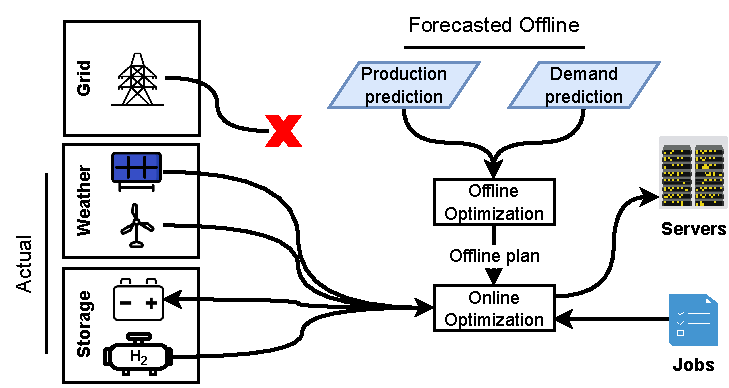
\includegraphics[scale=1]{Images/Introduction/Problem_overview_thesis.pdf}
    \caption[Problem overview]{Problem overview. Online receives an offline plan, the actual renewable production, and the users' jobs. It must define energy storage usage, job placement in the servers, and server speed.}
    \label{fig:introduction_problem}
\end{figure}

On the IT side, online receives the jobs from the users and must schedule them on the available servers. Online receives an offline plan for server configuration (machine on/off and speed). However, it can modify the server configuration to react to incoming events (e.g., more production, demand peak). Changing the speed of a server is possible due to the Dynamic Voltage and Frequency Scaling (DVFS) technique. DVFS allows servers' speed reduction, spending less energy. However, putting a job on a server with a decreased speed can impact the job QoS. On the other hand, DVFS also allows increasing CPU speed to run the jobs faster. To sum up, online must manage the battery (maintaining the SoC between thresholds and finishing the time window with the battery level close to the target), schedule the jobs, and balance the servers' speed.

This thesis' objectives are:
\begin{enumerate}
    \item Mixing offline and online decisions, dealing with the uncertainty coming from renewable production and workload demand. These decisions aim to improve QoS while meeting power constraints;
    \item Mixing power, scheduling, and server online decisions, turning the scheduling energy storage aware. This mix allows the scheduling to make better decisions than usual algorithms;
\end{enumerate}

These goals help to find a better trade-off between QoS and energy storage management, taking into account the power and demand predictions. Different contributions address these questions in this manuscript.

\section{Main contributions}

% Find the algorithms to deal with the uncertainties, improving QoS
\begin{center}
    \textbf{Defining offline power and IT decisions}
\end{center}
As illustrated in Figure \ref{fig:introduction_problem}, an important part is the offline plan. This plan must consider the power and demand predictions to define the actions for the next time window. We separate the problem into two parts. First, we present the optimization problem to define power engagement, giving a power prediction. This optimization problem results in expected renewable power production, energy storage usage, and expected SoC. The sum of the expected renewable power production and energy storage usage is named the power envelope. The second part is the IT servers' state (on/off) and speed definition. This optimization problem defines the state and speed according to the power envelope. The objective of this optimization problem is to maximize the servers' speed. The results of both optimizations are the input for the online module.

\begin{center}
    \textbf{Reacting to power fluctuations}
\end{center}
We propose a heuristic to react to the power fluctuations using the result of the offline plan as a guide. Since there is no perfect prediction, one source of divergence is the difference between the prediction and actual values. This divergence occurs in both power demand and production. Additionally, the offline model considers that the servers will maintain constant power usage. However, the server consumption can vary according to the scheduling and/or job. Yet, the scheduling can modify the battery usage to improve the QoS (e.g., avoiding killing jobs). Considering all these sources of power fluctuations, the heuristic must adapt the usage, aiming to approximate the state of charge of the target level at the end of the time window. Since this is an online problem, we can not re-run the offline optimization solution with the actual values. Therefore, we propose four policies to compensate for these divergences in the power envelope. Each one finds a different moment in the future to place the compensation. 

\begin{center}
    \textbf{Learning the actions to deal with power fluctuations}
\end{center}
The four compensation policies apply the same behavior throughout the entire execution. However, different moments inside the time window can demand distinct policies. So, the third contribution aims to learn when to use each policy. So, we introduce two Reinforcement Learning (RL) algorithms to discover the best mix of policies. Considering each policy as RL's action, we present the RL's state and reward. The premise of applying RL is that optimizing the decisions locally generates a global optimal. In other words, if the algorithm chooses the best action each time, in the end, we will have the best results. We implemented two well-known RL algorithms named Contextual Multi-Armed Bandit and Q-Learning. We present the learning results and a comparison between the RL algorithms and baseline choices. 

\begin{center}
    \textbf{Defining energy storage-aware scheduling using production and demand predictions}
\end{center}

Finally, the last contribution is an energy storage-aware scheduling heuristic. This algorithm is based on the well-known EASY-Backfilling. The algorithm is named BEASY (Battery-aware EASY backfilling). BEASY uses the predictions given by the offline to predict dangerous moments, where it must be careful in the scheduling. Furthermore, we introduce another level of validation, verifying if the servers allocated to the job would be available during the entire execution. Regarding power compensations, it creates several possible scenarios of production and demand using the forecasts. According to these scenarios, the heuristic finds the best moment to make the compensations. For example, BEASY tries to reduce the usage before the moments when the predictions indicate that the battery could be lower than a critical value. This heuristic mixes all decisions providing a well-balanced answer to the online multi-objective problem.

\begin{center}
    \textbf{Proposing a simulation environment}
\end{center}
A crucial step to simulate data center management is defining the workload, weather, and server configuration, in a complete simulation tool. Regarding the workload, some traces are used in literature, such as Google \cite{reiss2011google}, Parallel Workloads Archive \cite{feitelson2014experience}, and Alibaba \cite{wang2022characterizing}. We propose a trace from Parallel Workloads Archive named Metacentrum \cite{klusavcek2017real}. We detail the filtering process of this trace. Considering the weather, it is possible to collect data from everywhere in the world. We present the methodology to generate power production from a NASA trace, using the framework Renewables.ninja\footnote{https://www.renewables.ninja/} \cite{pfenninger2016long}. The third input is the server configuration. We demonstrate the data collected from a server in GRID5000\footnote{https://www.grid5000.fr} used in this thesis. Finally, we present the simulation tool named BATSIM\footnote{https://batsim.org/}, based on SIMGRID\footnote{https://simgrid.frama.io/}. We introduced in this simulation tool the modifications needed to manage battery and power production. The whole of these data and definitions allows future work inside and outside the Datazero2 project.

\section{Publications and Communication}

\hspace{0.5cm} \textbf{Accepted Peer Reviewed Conferences:}
\begin{itemize}
    \item I. F. de Nardin, P. Stolf and S. Caux, ``Adding Battery Awareness in EASY Backfilling'', 2023 IEEE 35th International Symposium on Computer Architecture and High Performance Computing (SBAC-PAD), Porto Alegre, Brazil, 2023 \cite{de2023adding}.
    \item I. F. de Nardin, P. Stolf and S. Caux, ``Analyzing Power Decisions in Data Center Powered by Renewable Sources'', 2022 IEEE 34th International Symposium on Computer Architecture and High Performance Computing (SBAC-PAD), Bordeaux, France, 2022, pp. 305-314 \cite{de2022analyzing};
    \item I. F. de Nardin, P. Stolf and S. Caux, ``Evaluation of Heuristics to Manage a Data Center Under Power Constraints'', 2022 IEEE 13th International Green and Sustainable Computing Conference (IGSC), Pittsburgh, PA, USA, 2022, pp. 1-8 \cite{de2022evaluation};
    \item I. F. de Nardin, P. Stolf and S. Caux, ``Mixing Offline and Online Electrical Decisions in Data Centers Powered by Renewable Sources'', IECON 2022 – 48th Annual Conference of the IEEE Industrial Electronics Society, Brussels, Belgium, 2022, pp. 1-6 \cite{de2022mixing};
    \item  I. F. de Nardin, P. Stolf and S. Caux, ``Smart Heuristics for Power Constraints in Data Centers Powered by Renewable Sources'', Conférence francophone d'informatique en Parallélisme, Architecture et Système (COMPAS 2022), Jul 2022, Amiens, France. paper 7 \cite{fontanadenardin:hal-03757548}.
\end{itemize}

\textbf{Others Disseminations:}
\begin{itemize}
    \item Talk: Analyzing Power Decisions in Data Center
    Powered by Renewable Sources, GreenDays@Lyon, March 2023.
\end{itemize}

\section{Dissertation Outline}
The remaining dissertation has the following organization:
\begin{itemize}
    \item[] \textbf{Chapter 2 - Context and Related Works:} This chapter presents the fundamentals to understand this dissertation. Considering the scope of the topic, the context consists of four parts. First, we introduce the context of global and ICT GHG emissions. Then, we describe renewable energy as an alternative to replace brown energy. After, we explain the usage of renewable to maintain a data center. Then, we define the uncertainties of weather and workload in a renewable-only data center. This last part also clarifies the importance of using predictions but with an online adaptation. After presenting the context, we introduce a list of works that solve part of our problem, highlighting the existing gaps in the state-of-the-art;
    \item[] \textbf{Chapter 3 - Modelling, Data, and Simulation:} In this chapter, we describe the model to deal with several elements that compose a renewable-only data center. Datazero2 creates a division between Offline and Online decisions. We present the model to deal with offline decisions using predicted power demand and production. Then, we detail the output of Offline used by the Online. Finally, we define the Online model, which englobes the job scheduling and modifications in the Offline plan. After describing the model, we explain the source of the different data (e.g., workload, weather, servers) applied in the simulations. We present an explanation of the work done in the traces of the literature. Finally, we present the simulation tools used in this work;
    \item[] \textbf{Chapter 4 - Introducing Power Compensations:} This chapter describes the proposed algorithm to react to power uncertainties. We created four heuristics to find the best place to compensate for battery changes, which aim to reduce the number of killed jobs and the distance between the battery level and the target level. The results presented are related to the publications \cite{de2022analyzing} and \cite{de2022mixing};
    \item[] \textbf{Chapter 5 - Learning Power Compensations:} This chapter presents the idea and the results of the introduction of Reinforcement Learning (RL) in the power compensation problem. We propose two RL algorithms (Q-Learning and Contextual Multi-Armed Bandit) to learn the best moment to compensate;
    \item[] \textbf{Chapter 6 - Adding Battery Awareness in EASY Backfilling:} This chapter explains a heuristic to mix scheduling and power compensation decisions. This heuristic is based on the EASY Backfilling scheduling algorithm but considers the battery's State of Charge to make better decisions. The results presented are related to the publication \cite{de2023adding};
    % \item[] \textbf{Chapter 7 - Middleware Integration:} This chapter presents the tools, frameworks, and approaches applied to integrate the algorithms in the Datazero2 middleware. We describe the work done to create a docker environment, allowing different actors to execute the middleware;
    \item[] \textbf{Chapter 7 - Conclusion and Perspectives:} Finally, in this chapter, we summarize the contributions of this work, providing a discussion about future works.
\end{itemize}


    \chapter{Context and Related Work}

\section{Datazero2}

\subsection{Offline Decision Modules}

\subsection{Online Decision Modules}

\section{IT Elements}

\subsection{Type of Jobs}

\subsection{Scheduling Algorithms}

\subsection{Energy consumption}

\section{Electrical Elements}

\subsection{Storages}

\subsection{Renewable Production}

\section{Literature Review}

\subsection{Discussion and Classification of the Literature}

    \chapter{Modelling, Data, and Simulation}
\label{cha:model}

\minitoc

\section{Introduction}

After describing the state-of-the-art, this chapter presents the models, data, and simulation tools used in this thesis. First, we focus on the model describing the offline and online scheduling problem. We explain what kind of information is exchanged between offline and online. After the model, we introduce the traces used in the experiments. These traces emulate a real environment regarding workload, weather, and platform. Finally, we detail the simulation tools, explaining the modifications needed to create the experimental environment.

\section{Model}

As presented in Chapter \ref{cha:related_work}, a gap in the state-of-the-art is the mix of offline and online. Figure \ref{fig:model} illustrates the architecture proposed by the Datazero2 project, mixing both decision levels \cite{Datazero}. Since this work is part of this project, we use the same architecture. There are four main modules: IT Decision Module (ITDM), Power Decision Module (PDM), Negotiation Module (NM), and Online Decision Module (ODM). ITDM, PDM, and NM are responsible for the offline decisions, and ODM manages the online actions. This thesis focuses on the Online Decision Module. However, we present in the following sections the optimizations made in offline modules to provide the data needed by ODM since we propose a mix between offline and online decisions.

Besides these four modules, Datazero2 also includes an event generator and a metronome. Both components are essential for the simulations. Event generator simulates the real events of a data center, such as job submissions, weather conditions, etc. It simply reads a file and sends the data to the bus. The metronome synchronizes the simulation messages. So, every component waits for the time evolution from the metronome. This thesis does not detail these components, concentrating on the decision modules and their interactions.

\begin{table*}[!htb]
\centering
% \scriptsize
\caption{General notations.}
\label{tab:notation_system}
\begin{tabular}{l|l}
    \hline
    Notation & Description \\\hline\hline
    % System
    $t$ & Time step (int)\\
    $T$ & Last time step (int)\\
    $\Delta t$ & Time step length (s)\\
    $T_{w}$ & Time window length (s)\\
    $P_{load}$ & Estimated power demand (kW)\\
    $u_{load}$ & Uncertainty of $P_{load}$\\
    $P_{prod}$ & Power production by all sources (kW)\\
    $P_{renew}$ & Power delivered by renewable sources (kW)\\
    $u_{renew}$ & Uncertainty of $P_{renew}$\\
    \hline
\end{tabular}
\end{table*}

Table \ref{tab:notation_system} presents the general notations and each following section introduces its own notations. Both offline and online use the time division from Figure \ref{fig:time_window}. The time window is the horizon of the offline plan. Offline considers the time window to define how far to predict weather and workload. In addition, it uses the time window to determine the planned actions. Our model divides the time window into several time steps, as represented in Figure \ref{fig:time_window} by the different $t$. The actions for power and server are constant inside the time step. For example, if a server is at some state in step $t=0$, it will remain at this state during the step duration.

\begin{figure}[!htb]
    \centering
    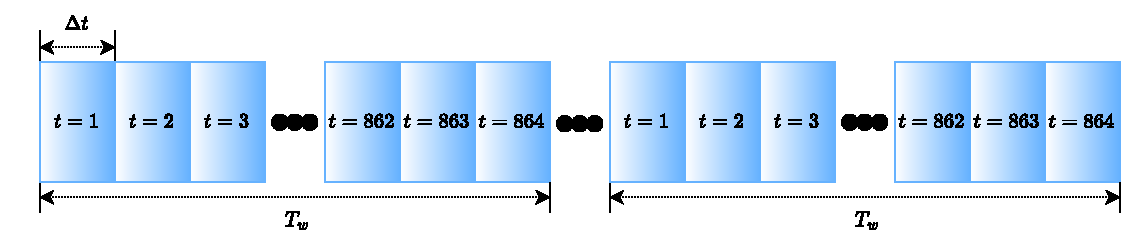
\includegraphics[scale=0.75]{Images/Model/Time window.pdf}
    \caption{Time window definition. It gives an example for a time window of 3 days.}
    \label{fig:time_window}
\end{figure}

\subsection{Offline Decision Modules}
\label{sec:offline_modules}

This section starts presenting the offline decision modules. First, we demonstrate how PDM and ITDM agree on a power envelope through NM. Then, we explain the power decisions from PDM, resulting in a power plan. Finally, we detail the ITDM, which defines the IT plan.

\subsubsection{Negotiation (NM)}
% Negotiation is a crucial step in Datazero2 architecture. A renewable-only data center introduces several constraints and decision variables. On the PDM side, it must approximate demand and production while considering long-term storage elements. For example, PDM can provide more power from hydrogen in a case with low renewable generation. However, PDM must evaluate the impact of its actions since the energy of the storage is finite. On the other hand, ITDM maximizes the Quality of Service. Thus, it demands more energy to run more servers at faster speeds. NM is between PDM and ITDM, trying to find an agreement. NM works iteratively. On each iteration, both PDM and ITDM propose a power envelope to NM, considering the objective of each module. A power envelope is a time series of the power production from the sources in a time window. While PDM tries to reduce the power envelope to control the storage, ITDM increases it to run more jobs faster. NM compares both envelope propositions and returns a new one. Then, each module verifies if they can use the proposed power envelope. They run several iterations until both agree or reach a timeout.

The negotiation Module is between PDM and ITDM, trying to find an agreement about the power profile. Since this thesis focuses on the online part, we simplify this process. We implemented the negotiation in three steps. First, ITDM proposes a power envelope $P_{load}$ based on the energy demanded to run a predicted workload. $P_{load}$ is a prediction from ITDM. We do not include it in this model, but we present in the following chapters how we generated it. Then, PDM takes this envelope and runs its optimization. It can degrade the power envelope to meet its objectives, resulting in a new power envelope $P_{prod}$. Finally, ITDM takes the PDM power production and finds the best server configuration that meets it. The following sections present the PDM and ITDM optimizations.

\subsubsection{Power Decision Module (PDM)}
Table \ref{tab:notation_power} gives the notations for PDM. PDM plans the renewable source engagement to provide the energy needed to maintain the IT elements running. A renewable-only data center introduces several constraints in power generation. Therefore, PDM must approximate the demanded power while considering long-term storage elements. For example, it can use more energy coming from hydrogen during the winter, which has lower power production, compensating for this usage in the summer, which has higher power generation. On the other hand, PDM can degrade the provided energy due to a lack of energy from storage and estimated renewable. In the context of Datazero, \citeauthor{haddad2019mixed} created the first model to solve this problem \cite{haddad2019mixed}. This thesis uses a similar model to PDM. Equation \ref{equ:model_energy} gives the power production from all renewable sources. Equation \ref{equ:renewable_power} indicates that $P_{renew}$ comes from wind and solar production. $P_{wt}(t)$, $P_{pv}(t)$, $P_{fc}(t)$, $P_{ez}(t)$, $P_{dch}(t)$, and $P_{ch}(t)$ are calculated using Equations \ref{equ:wind_turbines}, \ref{equ:panel_solar_with_temperature}, \ref{equ:hydrogen_full_cell}, \ref{equ:hydrogen_electrolyzer} and \ref{equ:battery_energy} from Section \ref{sec:related_work_electrical_elements}. Batteries are reversible, which means that they can charge ($P_{ch}(t)$) and discharge ($P_{dch}(t)$) energy. Similarly, hydrogen can be considered reversible using an electrolyzer to charge ($P_{ez}(t)$) and a fuel cell to discharge ($P_{fc}(t)$).

\begin{table*}[!htb]
\centering
% \scriptsize
\caption{Notations for PDM.}
\label{tab:notation_power}
\begin{tabular}{l|l}
    \hline
    Notation & Description \\\hline\hline
    % Power
    $P_{wt}$ & Power delivered by wind turbines (kW)\\
    $P_{pv}$ & Power delivered by solar panels (kW)\\
    $P_{fc}$ & Power delivered by fuel cell (kW)\\
    $P_{ez}$ & Power put into electrolyzer to generate hydrogen (kW)\\
    $P_{dch}$ & Battery discharging power (kW)\\
    $P_{ch}$ & Battery charging power (kW)\\
    $\eta_{ch}$ & Battery charge efficiency (\%)\\
    $\eta_{dch}$ & Battery discharge efficiency (\%)\\
    $SoC$ & State of Charge (\%)\\
    $LoH$ & Level of Hydrogen (kg)\\
    $SoC_{max}$ & Maximal battery State of Charge (\%)\\
    $SoC_{min}$ & Minimal battery State of Charge (\%)\\
    $B_{size}$ & Size of the battery (kWh)\\
    $LoH_{max}$ & H2 tank limit (kg)\\
    $P_{dch_{max}}$ & Battery maximum discharging power (kW)\\
    $P_{ch_{max}}$ & Battery maximum charging power (kW)\\
    $P_{fc_{max}}$ & Fuel cell maximum charging power (kW)\\
    $P_{ez_{min}}$ & Electrolyzer minimum charging power (kW)\\
    $P_{ez_{max}}$ & Electrolyzer maximum charging power (kW)\\
    $SoC_{target}$ & Target State of Charge at the end of the time window (\%)\\
    $LoH_{target}$ & Target Level of Hydrogen at the end of the time window (kg)\\
    $rf$ & Relax factor (float) \\
    $P^{real}_{load}$ & Real power demand (kW)\\
    $P^{real}_{renew}$ & Estimated power demand (kW)\\
    \hline
\end{tabular}
\end{table*}

\begin{equation}
    \label{equ:model_energy}
    P_{prod}(t) = P_{renew}(t) + (P_{fc}(t) + P_{dch}(t) - P_{ez}(t) - P_{ch}(t)), \quad \forall 0 \le t \le T
\end{equation}

\begin{equation}
    \label{equ:renewable_power}
    P_{renew}(t) = P_{wt}(t) + P_{pv}(t), \quad \forall 0 \le t \le T
\end{equation}

$P_{ch}(t)$, $P_{dch}(t)$, $P_{ez}(t)$, and $P_{fc}(t)$ are the decision variables in Equation \ref{equ:model_energy}, since $P_{wt}(t)$ and $P_{pv}(t)$ come from wind speed and solar irradiance. As presented in Section \ref{sec:related_work_electrical_elements}, $SoC(t)$ depends on the charge $P_{ch}(t)$ and discharge $P_{dch}(t)$ (see Equation \ref{equ:battery_energy}), and $LoH(t)$ depends on the power of the electrolyzer $P_{ez}(t)$ and fuel cells $P_{fc}(t)$ (see Equation \ref{equ:hydrogen_level}). Regarding $SoC(t)$, the state of charge must be between the boundaries $SoC_{min}$ and $SoC_{max}$, as written in Equation \ref{equ:battery_boundaries}. These boundaries help to extend the battery lifespan \cite{xu2016modeling}.

\begin{equation}
    \label{equ:battery_boundaries}
    SoC_{min} \leq SoC(t) \leq SoC_{max}, \quad \forall 0 \le t \le T
\end{equation}

On the other hand, hydrogen only has the tank size as a boundary. So, Equation \ref{equ:hydrogen_boundaries} presents the level of hydrogen constraint.

\begin{equation}
    \label{equ:hydrogen_boundaries}
    0 \leq LoH(t) \leq LoH_{max}, \quad \forall 0 \le t \le T
\end{equation}

Considering the power to charge/discharge the batteries, both have upper limits. These boundaries avoid destroying the battery. So, we introduce constraints \ref{equ:discharge_boundary} and \ref{equ:charge_boundary}.

\begin{equation}
    \label{equ:discharge_boundary}
    0 \leq P_{dch}(t) \leq P_{dch_{max}}, \quad \forall 0 \le t \le T
\end{equation}

\begin{equation}
    \label{equ:charge_boundary}
    0 \leq P_{ch}(t) \leq P_{ch_{max}}, \quad \forall 0 \le t \le T
\end{equation}

Fuel cells and electrolyzers also have boundaries. While fuel cells have only a maximum limit, electrolyzers have an operating range. So, Equations \ref{equ:fuelcells_boundary} and \ref{equ:electrolyzer_boundary} present them.

\begin{equation}
    \label{equ:fuelcells_boundary}
    0 \leq P_{fc}(t) \leq P_{fc_{max}}, \quad \forall 0 \le t \le T
\end{equation}

\begin{equation}
    \label{equ:electrolyzer_boundary}
    P_{ez_{min}} \leq P_{ez}(t) \leq P_{ez_{max}}, \quad \forall 0 \le t \le T
\end{equation}

Another important constraint is the target hydrogen and battery level at the end of the time window ($SoC(T)$). Using only the previous constraints, the model can use all the power available in the energy storages, drying them but providing a high quality of service. However, Figure \ref{fig:time_window} shows that the time windows are chained. So, the next time window will not have energy in the storage. Therefore, we introduce these targets. So, the state of charge and level of hydrogen in the last step of the time window must respect Equations \ref{equ:soc_target} and \ref{equ:loh_target}. These targets can be the subject of another optimization or indicated by hand by the data center manager. Furthermore, the targets must consider the long-term perspective, such as seasons with lower/higher production, the peak of demand over an external event, etc. 

\begin{equation}
    \label{equ:soc_target}
    SoC(T) \ge SoC_{target}
\end{equation}

\begin{equation}
    \label{equ:loh_target}
    LoH(T) \ge LoH_{target}
\end{equation}

Finally, the objective is to approximate the power production to the power demand. So, Equation \ref{equ:load_production} shows the relation between demand ($P_{load}$) and generation ($P_{prod}$). The optimization finds a solution where the production is higher or equal to the demand. However, it can not match both in every case. Therefore, the model introduces a demand degradation using a relax factor ($rf$). With the relax factor equal to 0, it matches demand and production. Increasing the relax factor would reduce the power given to IT, impacting the QoS. Thus, the objective is reducing the relax factor, as presented in Equation \ref{equ:objective_function}.

\begin{equation}
    \label{equ:load_production}
    P_{prod}(t) \ge (1 - rf) \times P_{load}, \quad \forall 0 \le t \le T
\end{equation}

\begin{equation}
    \label{equ:objective_function}
    \mathbf{minimize}\ rf
\end{equation}

% \citeauthor{haddad2019mixed} presented a way to linearize this model, allowing it to be solved using MILP. This thesis used the \citeauthor{haddad2019mixed} proposition to solve it using MILP. 

% \begin{equation}
%     \label{equ:model_wind_turbines}
%     P_{WT}(t) = \begin{cases}
%         0 & v \leq v_{in} \text{ or } v(t) > v_{out} \\
%         P_{WT,rated} \times \frac{v^{3}(t) - v^{3}_{in}}{v^{3}_{rated} - v^{3}_{in}} & v_{in} < v(t) \leq v_{rated} \\
%         P_{WT,rated} & v_{rated} < v(t) \leq v_{out}
%     \end{cases}
% \end{equation}

% \begin{equation}
%     \label{equ:model_panel_solar_with_temperature}
%     P_{pv}(t) = P_{R,PV} \times (R / R_{ref}) \times \eta_{PV}
% \end{equation}

% \begin{equation}
%     \label{equ:model_battery_energy}
%     E_{bat}(t) = (E_{bat}(t-1) \times (1 - \sigma)) + (P_{ch}(t-1) \times \eta_{ch} \times \Delta t) - (P_{dch}(t-1) \times \eta_{dch} \times \Delta t)
% \end{equation}
% \begin{equation}
%     \label{equ:model_battery_state_of_charge}
%     SoC(t) = \frac{E_{bat}(t)}{C_{bat}} \times 100
% \end{equation}

% \begin{equation}
%     \label{equ:model_hydrogen_electrolyzer}
%     P_{ez}(t) \times \Delta t = \frac{HH_{h_{2}} \times Q_{ez}(t)}{\eta_{ez}}
% \end{equation}

% \begin{equation}
%     \label{equ:model_hydrogen_full_cell}
%     P_{fc}(t) \times \Delta t = LH_{h_{2}} \times Q_{fc}(t) \times \eta_{fc}
% \end{equation}

% \begin{equation}
%     \label{equ:model_hydrogen_level}
%     LoH(t) = LoH(t-1) + Q_{ez}(t-1) - Q_{fc}(t-1)
% \end{equation}

\subsubsection{IT Decision Module (ITDM)}

ITDM aims to maximize QoS, translating $P_{prod}(t)$ into server configuration. Table \ref{tab:notation_it} introduces the notations for ITDM. Server configuration means the CPU P-state of the servers. For each P-state, the server has a speed (in flops \cite{hunger2005floating}) and power consumption (in W). Table \ref{tab:servers} exemplifies this relation. The CPU frequency range is discrete, although some works define it to be continuous \cite{saha2012experimental}. ITDM must find the best combination of servers off and on at some speed that uses equal or less energy than the power envelope $P_{prod}(t)$. Thus, given a data center with $S$ servers, each server $s$ has a list of states $D_s$. Each state $d$ in $D_s$ has a speed $F_{s,d}$ and a power $P_{s,d}$. $D_{s,d}(t)$ is the boolean decision variable that indicates that the server $s$ is at state $d$ at step $t$. The sleep state has a different state $Dsl_{s}(t)$ which helps to identify the transition between sleeping and running. The transition between on$\rightarrow$off is called sedating and off$\rightarrow$on is waking.

\begin{table*}[!htb]
\centering
% \scriptsize
\caption{Notations for ITDM.}
\label{tab:notation_it}
\begin{tabular}{l|l}
    \hline
    Notation & Description \\\hline\hline
    $S$ & Servers (list) \\
    $N_{S}$ & Number of servers (int) \\
    $s$ & Server index (int) \\
    $D_s$ & States of server s (list) \\
    $N_{D_{s}}$ & Number of states of server s (int) \\
    $d$ & State index (int) \\
    $F_{s,d}$ & Speed of server $s$ at state $d$ (Flops)\\
    $P_{s,d}$ & Power of server $s$ at state $d$ (W)\\
    $D_{s,d}$ & Indicates that the server $s$ is at state $d$ (boolean)\\
    $Dsl_{s}$ & Indicates that the server $s$ is sleeping (boolean)\\
    $wa_s$ & Indicates if the server is waking, transiting from off$\rightarrow$on (boolean) \\
    $T_{wa_s}$ & Transition time from off$\rightarrow$on (s) \\
    $se_s$ & Indicates if the server is being sedate, transiting from on$\rightarrow$off (boolean) \\
    $T_{se_s}$ & Transition time from on$\rightarrow$off (s) \\    
    $E_{tot}$ & Energy total spent by the servers (J) \\
    $E_{run}$ & Energy spent by the running servers (J) \\
    $E_{wak}$ & Energy spent by waking the servers (J) \\
    $E_{sed}$ & Energy spent by sedating the servers (J) \\
    $E_{sle}$ & Energy spent by the sleeping servers (J) \\
    \hline
\end{tabular}
\end{table*}

\begin{table}[!htb]
\centering
\caption[Server definition example]{Server definition example. The power is for all server's processors busy. The values are from Grid5000's Parasilo server~\cite{dacosta:hal-03453537v1, dacostakeynote}.}
\label{tab:servers}
\begin{tabular}{c|c|c}
    \hline
    State        & Power (W) & Speed (Gflops) \\ \hline\hline
    0                       & 221.77                   & 38.4                          \\
    1                       & 216.77                   & 37.78                         \\
    2                       & 213.58                   & 36.93                         \\
    3                       & 208.90                   & 36.01                         \\
    4                       & 204.45                   & 34.72                         \\
    5                       & 200.62                   & 33.90                         \\
    6                       & 197.28                   & 32.84                         \\
    7                       & 192.49                   & 31.72                         \\
    8                       & 184.26                   & 30.63                         \\
    9                       & 182.04                   & 29.25                         \\
    10                      & 179.75                   & 27.93                         \\
    11                      & 176.70                   & 26.37                         \\
    12                      & 175.53                   & 25.01                         \\
    13 (sleep)              & 4.5                      & 0                             \\ \hline
\end{tabular}
\end{table}

First, Equation \ref{equ:one_state_only} ensures only one state per time $t$. The state can be anyone from $D_{s,d}$ to indicate a P-state, or $Dsl_{s}(t)$ to specify the sleep state. Since both variables are booleans (accepting only 0 or 1 values), summing them must be equal to 1 (at least one must be true). Both $D_{s,d}$ and $Dsl_{s}(t)$ are the only decision variables in the ITDM model.

\begin{equation}
    \label{equ:one_state_only}
    Dsl_{s}(t) + \sum_{d=0}^{N_{D_{s}}} D_{s,d}(t) = 1, \quad \forall 0 \le t \le T, \forall 0 \le s \le N_{S}
\end{equation}

Then, we must model the sedating and waking transitions. These transitions take time and spend energy. During these transitions, the servers are unavailable to run jobs. So, Equations \ref{equ:transition_wake} and \ref{equ:transition_sedating} model the waking transition (off$\rightarrow$on) and the sedating transition (on$\rightarrow$off), respectively. For example, Equation \ref{equ:transition_wake} verifies if the previous state is sleeping ($Dsl_{s}(t-1) = 1$) and now is not sleeping ($Dsl_{s}(t) = 0$). So the result of $Dsl_{s}(t-1) - Dsl_{s}(t)$ will be $1$, which indicates that the server $s$ is waking. If both are $0$ or $1$, the result is $0$, implying that the server is not transiting. If the previous state is not sleeping ($Dsl_{s}(t-1) = 0$) and now is sleeping ($Dsl_{s}(t) = 1$), the result will be $-1$. However, the $\max (0)$ function will put 0 as $wa_s(t)$. Equation \ref{equ:transition_sedating} does the same but inverts the order of states.

\begin{equation}
    \label{equ:transition_wake}
    wa_{s}(t) = \max(0, (Dsl_{s}(t-1) - Dsl_{s}(t))), \quad \forall 0 \le t \le T, \forall 0 \le s \le N_{S}
\end{equation}

\begin{equation}
    \label{equ:transition_sedating}
    se_{s}(t) = \max(0, (Dsl_{s}(t) - Dsl_{s}(t-1))), \quad \forall 0 \le t \le T, \forall 0 \le s \le N_{S}
\end{equation}

Equation \ref{equ:ITDM_energy_less_envelope} introduces the power constraint. We transform the power into energy (multiplying $P_{prod}(t)$ by $\Delta t$) because we are dealing with the transitions. Thus, the power from a server is not constant inside a time step (e.g., in the waking transition, first a server spent energy turning on and just after running jobs). Since $E_{tot}(t)$ is in J and the energy generated ($P_{prod}(t) \times \Delta t$) is in kJ, we transformed the generation into J by multiplying by 1000. $E_{tot}(t)$ is the total energy spent by the servers calculated using Equation \ref{equ:ITDM_energy_usage}. This equation sums the expended energy by running, waking, sedating, and sleeping states.

\begin{equation}
    \label{equ:ITDM_energy_less_envelope}
    P_{prod}(t) \times \Delta t \times 1000 \ge E_{tot}(t), \quad \forall 0 \le t \le T
\end{equation}

\begin{equation}
    \label{equ:ITDM_energy_usage}
    E_{tot}(t) = E_{run}(t) + E_{wak}(t) + E_{sed}(t) + E_{sle}(t), \quad \forall 0 \le t \le T
\end{equation}

Equations \ref{equ:ITDM_energy_running}, \ref{equ:ITDM_energy_sleeping}, \ref{equ:ITDM_energy_sedating}, and \ref{equ:ITDM_energy_waking} demonstrate the energy of each state. Equation \ref{equ:ITDM_energy_running} verifies if the server is in one of the possible P-states $D_{s,d}$. If so, it multiplies the power by the time in this state. For calculating the time in the state, the equation verifies if the server is waking, removing the transition time if so. Equation \ref{equ:ITDM_energy_sleeping} does the same for the sleeping state, considering the sedating transition. Equations \ref{equ:ITDM_energy_waking} and \ref{equ:ITDM_energy_sedating} are simpler, just multiplying the power usage in the transition state by the time, if the server is in the state.

\begin{equation}
    \label{equ:ITDM_energy_running}
    E_{run}(t) = \sum_{s=0}^{N_{S}}\sum_{d=0}^{N_{D_{s}}} D_{s,d}(t) \times P_{s,d} \times (\Delta t - (wa_{s}(t) \times T_{wa_{s}})), \quad \forall 0 \le t \le T
\end{equation}

\begin{equation}
    \label{equ:ITDM_energy_sleeping}
    E_{sle}(t) = \sum_{s=0}^{N_{S}} Dsl_{s}(t) \times P_{sl_{s}} \times (\Delta t - (se_{s}(t) \times T_{se_{s}})), \quad \forall 0 \le t \le T
\end{equation}

\begin{equation}
    \label{equ:ITDM_energy_waking}
    E_{wak}(t) = \sum_{s=0}^{N_{S}} wa_{s}(t) \times T_{wa_{s}} \times P_{wa_{s}}, \quad \forall 0 \le t \le T
\end{equation}

\begin{equation}
    \label{equ:ITDM_energy_sedating}
    E_{sed}(t) = \sum_{s=0}^{N_{S}} se_{s}(t) \times T_{se_{s}} \times P_{se_{s}}, \quad \forall 0 \le t \le T
\end{equation}

Finally, Equation \ref{equ:ITDM_objective} demonstrates the objective function of ITDM. The objective is to maximize the total flops executed by the server. We do not consider idle servers here, since we do not make offline scheduling. So, when the server is running, we consider that it is providing all the flops possible at state $D_{s,d}$. Like in the energy consumption in the running state (Equation \ref{equ:ITDM_energy_running}), the objective function also considers the transition state for reducing the total flops delivered by the server.

\begin{equation}
    \label{equ:ITDM_objective}
    \mathbf{maximize} \sum_{t=0}^{T}\sum_{s=0}^{N_{S}}\sum_{d=0}^{N_{D_{s}}} D_{s,d}(t) \times F_{s,d} \times (\Delta t - (wa_{s}(t) \times T_{wa_{s}}))
\end{equation}

% Then, Equation \ref{equ:server_objective} tries to maximize the flops possible, while Equation \ref{equ:energy_less_equal_available} is a constraint to maintain the power lesser or equal to the envelope. Equation \ref{equ:only_one_state} assures that the server $s$ will be at only one state $d$ at time $t$. This model is also solved using MILP.

% \begin{equation}
%     \mathbf{maximize} \sum _{t=0}^{T}\sum _{s=0}^{S}\sum _{d=0}^{D_s} D_{s,d}(t) \times F_{s,d}
%     \label{equ:server_objective}
% \end{equation}
% \begin{equation}
%     \sum_{s=0}^{S} \sum_{d=0}^{D_s} P_{s,d} \times D_{s,d}(t) \leq P_{prod}(t), \quad \forall 0 \le t \le T
%     \label{equ:energy_less_equal_available}
% \end{equation}
% \begin{equation}
%     \sum_{s=0}^{S} \sum_{d=0}^{D_s} D_{s,d}(t) = 1, \quad \forall 0 \le t \le T
%     \label{equ:only_one_state}
% \end{equation}

\subsection{Offline Plan}
\label{sec:offline_plan}

The PDM and ITDM optimizations result in a plan for the next time window, providing two time series: The power plan (PDM) and the IT plan (ITDM), as follows:

\begin{itemize}
    \item Power plan (PDM)
    \begin{itemize}
        \item Time step ($t$);
        \item For battery (for every $t$):
        \begin{itemize}
            \item Power usage ($P_{dch}(t)$ and $P_{ch}(t)$);
            \item Expected storage level ($SoC(t)$);
        \end{itemize}
        \item For hydrogen (for every $t$):
        \begin{itemize}
            \item Power usage ($P_{fc}(t)$ and $P_{ez}(t)$);
            \item Expected storage level ($LoH(t)$);
        \end{itemize}
        \item For solar panels and wind turbines (for every $t$):
        \begin{itemize}
            \item Estimated renewable power production ($P_{renew}(t)$);
            \item Power production uncertainty ($u_{renew}(t)$);
        \end{itemize}
    \end{itemize}
    \item IT plan (ITDM)
    \begin{itemize}
        \item Time step ($t$);
        \item For each server (for every $t$):
        \begin{itemize}
            \item P-state ($D_{s,d}(t)$ and $Dsl_{s}(t)$);
        \end{itemize}
        \item Estimated power demand ($P_{load}(t)$) (for every $t$);
        \item Power demand uncertainty ($u_{load}(t)$) (for every $t$);
    \end{itemize}
\end{itemize}

$u_{renew}$ and $u_{load}$ indicate confidence in the prediction. They give the range that the actual values can be. For example, let's say $P_{load}(t) = 500$ and $u_{load}(t) = 200$. So, the real value of $P_{load}(t)$ ($P^{real}_{load}(t)$) is between 300 and 700 ($P^{real}_{load}(t) = P_{load}(t) \pm u_{load}(t)$). Equations \ref{equ:uncertainty_power} and \ref{equ:uncertainty_load} present the possible actual values interval.

\begin{equation}
    P_{renew}(t) \times -u_{renew}(t) \le P^{real}_{renew}(t) \le P_{renew}((t)) \times u_{renew}(t), \quad \forall 0 \le t \le T
    \label{equ:uncertainty_power}
\end{equation}

\begin{equation}
    P_{load}(t) \times -u_{load}(t) \le P^{real}_{load}(t) \le P_{load}((t)) \times u_{load}(t), \quad \forall 0 \le t \le T
    \label{equ:uncertainty_load}
\end{equation}

So, PDM and ITDM send this plan to ODM, which uses it as a guide for real-time decisions. However, the following sections present the reasons for changing this plan.

\subsection{Online Decision Module (ODM)}
\label{sec:ODM}
% This section describes the Online Decision Module (ODM) in three parts. First, we detail the scheduling algorithms used in ODM implementation. Then, we explain the power plan modifications, focusing on the reasons for modifying the plan. Finally, we present the idea for transforming the power modifications into IT modifications.

ODM is a power-aware scheduler. A power-aware scheduler means having all responsibilities described in Section \ref{sec:related_work_it_elements} while managing electrical elements. In this section, we present the job scheduler and the modifications in the offline plan. Table \ref{tab:notation_job} introduces the notations for ODM.

\begin{table*}[!htb]
\centering
% \scriptsize
\caption{Notations for online scheduling and adaptations.}
\label{tab:notation_job}
\begin{tabular}{l|p{12cm}}
    \hline
    Notation & Description \\\hline\hline
    $Q$ & Queue of jobs (list)\\
    $j$ & Job index (int)\\
    $Wall_j$ & Walltime of job $j$ (s)\\
    $Wait_j$ & Waiting time of job $j$ (s)\\
    $Sb_j$ & Submission time of job $j$ (s)\\
    $Ex_j$ & Execution time of job $j$ (s)\\
    $Dfl_j$ & Demanded flops of job $j$ (flop)\\
    $R_j$ & Number of resources requested by job $j$ (int) \\
    $Size_j$ & Job $j$ size (float)\\
    $bsld_j$ & Bounded Slowdown of job $j$ (float)\\
    $Gfl_j$ & Flops processed by the job $j$ (flops)\\
    $F'_{s}$ & Server speed for job size estimation (flops)\\
    $\epsilon_{u}$ & User execution time estimation error (float)\\
    $\Delta E_{bat}$ & Difference of target and calculated battery energy at the end of the time window (kWh)\\
    $E_{comp}$ & Energy to compensate (kWh)\\
    \hline
\end{tabular}
\end{table*}

\subsubsection{Job scheduler}

Since the offline in the model does not know the jobs exactly, it can not execute the job scheduling. Therefore, ODM must define the scheduling. The job scheduler's objective is to maximize the number of finished jobs, considering the power constraints. It does not know exactly when the jobs will arrive. As soon as a job arrives, the scheduler places it in a waiting queue $Q$. Each job $j$ in the waiting queue $Q$ is composed by submission time ($Sb_j$), walltime ($Wall_j$), and the number of resources requested ($R_j$). Walltime is the maximum execution time allowed for the job. The job executes flops ($Dfl_j$), but it is discovered only after the job execution.

After placing the job in the waiting queue, the scheduler must select which job will start. For selecting the next job to place, the scheduler must sort the queue $Q$. This sort puts the more important jobs in front, according to a specified rule. One rule can consider the jobs' size, using Equation \ref{equ:jobs_size}. Since the scheduler does not know the real size, it estimates using the walltime and number of resources requested.

\begin{equation}
    Size_j = Wall_j \times R_j
    \label{equ:jobs_size}
\end{equation}

Another way to sort the waiting queue $Q$ is using Bounded Slowdown. Equation \ref{equ:slowdown} demonstrates how to calculate the Bounded Slowdown. It estimates the ratio between the total time a job stays in the system and its actual processing time. This order helps to let a job wait proportionately to its size. $\tau$ is a constant to avoid smaller jobs from reaching a very high Bounded Slowdown. Since the scheduler does not know the actual size, Equation \ref{equ:slowdown} uses the walltime as size.

\begin{equation}
    bsld_j = \max(\frac{Wait_j + Wall_j}{\max(Wall_j, \tau)}, 1)
    \label{equ:slowdown}
\end{equation}

After sorting the queue, it places the front job in $R_j$ servers. Due to a possible heterogeneous data center, the scheduler takes first the servers with higher speed. After starting, $D_{s,d}$ controls how fast the job will finish. The scheduler considers a job as a mass (unknown) flops $Dfl_j$. So, increasing the speed $D_{s,d}$ increases the number of flops processed by the server and reduces the execution time $Ex_j$. On the other hand, reducing the speed reduces the server's flops and increases the execution time. Constraint \ref{equ:walltime} verifies if the execution time is lower than the walltime $Wall_j$. The moment when the execution time becomes equal to or greater than the walltime, the scheduler kills the job. The job finishes correctly when it executes all its flops $Dfl_j$ before the walltime $Wall_j$. 

\begin{equation}
    Ex_j < Wall_j
    \label{equ:walltime}
\end{equation}

\subsubsection{Modifying Offline Plan}

An important part of ODM is adapting the offline plan. The offline plan gives a guide in a predicted scenario, but the reality can be different. The main reason for adaptations is due to power production and demand variations. There are three sources of variation: IT consumption, renewable production, and scheduling adaptations. 

The IT consumption is the difference between the ITDM planned usage and the real usage. Since ITDM does not know the real scheduling, it considers the worst-case where the server usage is the higher possible. Equation \ref{equ:cpu_usage} demonstrates the relation of the power consumption at an instant according to the CPU. Inside a time step $t$, the server's CPU usage can vary according to the jobs. Figure \ref{fig:energy_consumption} illustrates this difference due to the job variance. Since we consider the worst-case in ITDM, the real energy usage is always lower or equal to the predicted.

\begin{figure}[!htb]
    \centering
    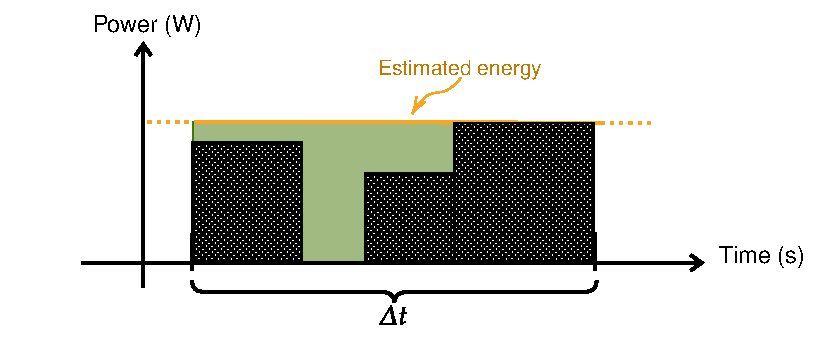
\includegraphics[scale=0.8]{Images/Model/energy_consumption.pdf}
    \caption{Energy consumption comparison between predicted and real. The black boxes are jobs. The green area is the energy predicted, but not used.}
    \label{fig:energy_consumption}
\end{figure}

The renewable production variation comes from the wind and solar variations. 
% This variance comes from the uncertainties presented in Section \ref{sec:weather_uncertainties}. 
These uncertainties can increase or decrease power generation $P_{renew}$. Finally, the scheduler adapts the server configuration to improve the QoS. Since the objective of the scheduling is to maximize the finished jobs, it must modify the offline plan. For example, if a job is running on a server, but the IT offline plan indicates putting this server to sleep, it would kill the job. So, ODM can change this decision, using more energy now and maintaining the job running. Another case is considering the speed given to the job. Letting a job in a server with a slower P-state can increase the execution time ($Ex_j$), violating Constraint \ref{equ:walltime} and killing the job. A way to reduce this possibility is by using Equation \ref{equ:avoid_walltime}. This equation verifies the minimum speed to complete the remaining job's flops. 

\begin{equation}
    (Wall_j - Ex_j) \times D_{s,d} \times F_{s,d} \ge Dfl'_j - Gfl_j
    \label{equ:avoid_walltime}
\end{equation}

Since ODM does not know the job's flops exactly, it can estimate using the walltime. Equation \ref{equ:estimated_job_size} shows a way for estimating $Dfl'_j$, similar to \cite{takizawa2020effect}. $F'_{s}$ is a fixed speed applied to the job. $\epsilon_{u}$ is a user error because the user can overestimate the execution time. We do not consider the walltime underestimation, because this always leads to killing the job (respecting Equation \ref{equ:walltime}). \citeauthor{takizawa2020effect} calculate $\epsilon_{u}$ for each user, using previous users' requests. Even if Equation \ref{equ:avoid_walltime} does not exactly use the real size, it is a good way to balance the states of a job.

\begin{equation}
    \label{equ:estimated_job_size}
    Dfl'_j = wall_j \times F'_{s} \times \epsilon_{u}
\end{equation}

The batteries smooth these variations, providing the power needed in case of underproduction or absorbing the generation excess. At the end of time step $t$, the $SoC(t)$ can be different from the prediction. Therefore, ODM recalculates all future $SoC$ using Equations \ref{equ:battery_energy} and \ref{equ:battery_state_of_charge}. With the $SoC(T)$ updated, Equation \ref{equ:delta_energy} can estimate how far the SoC at the end of the time window will be from the target. This equation gives a value of energy (in kWh). A positive $\Delta E_{bat}$ means that the battery will have more energy than predicted, allowing the scheduler to use this excess to run more jobs or speed up the servers. On the other hand, a negative $\Delta E_{bat}$ means that the battery will have less energy than predicted. In this case, ODM must reduce future usage to approximate $SoC(T)$ to $SoC_{target}$.

\begin{equation}
    \label{equ:delta_energy}
    \Delta E_{bat} = \frac{SoC(T) - SoC_{target}}{100}\times C_{bat}
\end{equation}

Then, ODM calculates how much energy it can compensate, using Equation \ref{equ:energy_battery}. This equation considers the loss in the process of charge/discharge. 

\begin{equation}
    \label{equ:energy_battery}
    E_{comp} = \begin{cases}
        \frac{\Delta E_{bat}}{\eta_{ch}} & \Delta E_{bat} > 0 \\
        \frac{\Delta E_{bat}}{\eta_{dch}} & \Delta E_{bat} < 0 \\
    \end{cases}
\end{equation}

Finally, ODM must modify futures $P_{dch}$ and $P_{ch}$ to use $E_{comp}$. We focus on battery modifications since it is faster to make online decisions on it. Hydrogen is not too reactive. We proposed some ways to deal with it in the following chapters. Since ODM modifies $P_{dch}$ and $P_{ch}$, $P_{prod}$ will also change (see Equation \ref{equ:model_energy}). So, ODM must adapt the IT plan (servers' states $D_{s,d}$) to meet the new $P_{prod}$. The algorithm to modify $D_{s,d}$ on-the-fly is also presented in the following chapters. This modification must respect the Constraint \ref{equ:ITDM_energy_less_envelope}.

\section{Data}
After describing the models, we describe the data used to simulate our environment. Our simulators expect three data: workload, weather, and platform. We explain the source of each one in the following sections. 

\subsection{Workload Trace}
\label{sec:workload_trace}

Workload trace is a log of job submissions in a resource (servers) provider. Some trace examples are Microsoft Azure \cite{cortez2017resource}, Google \cite{reiss2011google}, and Alibaba \cite{wang2022characterizing}. Regarding HPC, \citeauthor{feitelson2014experience} proposed the SWF format, which allows the data center providers to distribute logs to the research community \cite{feitelson2014experience}. In SWF, each line is a job with the fields separated by whitespace. Each line contains the following fields \cite{feitelson2014experience}:
\begin{itemize}
    \item \textit{Job Number}: The job ID starting with 1;
    \item \textit{Submit Time}: The submission time. The first job has 0 as submit time, and the following jobs use the first job as reference (in seconds);
    \item \textit{Wait Time}: How long the job waited in the queue (in seconds);
    \item \textit{Run Time}: The execution time in the data center (in seconds);
    \item \textit{Number of Allocated Processors}: The number of processors allocated to the job (integer);
    \item \textit{Average CPU Time Used}: The time that the job used the CPU. It is the average from all processors (integer);
    \item \textit{Used Memory}: The used memory, also average from all processors (kilobytes);
    \item \textit{Requested Number of Processors}: The number of processors requested by the user (integer);
    \item \textit{Requested Time}: This is the walltime (seconds);
    \item \textit{Requested Memory}: Requested memory per processor  (kilobytes);
    \item \textit{Status}: 1 if the job was completed, 0 if it failed, and 5 if canceled;
    \item \textit{User ID}: The user ID. Can be used to identify different jobs from the same user (integer);
    \item \textit{Group ID}: A group ID (some systems control the group and not the user ID) (integer);
    \item \textit{Executable (Application) Number}: Can link different jobs from the same application (integer);
    \item \textit{Queue Number}: Indicates in which queue the job was allocated (integer);
    \item \textit{Partition Number}: Indicates in which partition the job was allocated. For example, it is possible to use partition numbers to identify which machine in a cluster was used (integer);
    \item \textit{Preceding Job Number}: Indicates the number of a previous job in the workload, such that the current job can only start after the termination of this preceding job (integer);
    \item \textit{Think Time from Preceding Job}: The time between this job and the Preceding Job (seconds);
\end{itemize}

It is not mandatory to insert all information in a SWF file. Currently, Parallel Workloads Archive\footnote{https://www.cs.huji.ac.il/labs/parallel/workload/index.html} has 40 traces in SWF format. We chose the MetaCentrum2 workload trace from the Czech National Grid Organization \cite{klusavcek2015real}. MetaCentrum is a grid with resources in several cities in the Czech Republic. They have 19 clusters with 495 nodes and 8412 cores in total. Nodes are individual machines or servers within a cluster. Each node can have its own set of resources such as CPU, memory, storage, and network connectivity. A core refers to a processing unit within a CPU (Central Processing Unit). Modern CPUs often have multiple cores, allowing them to perform multiple tasks simultaneously. The trace has 5,731,100 jobs from January 2013 to April 2015. Metacentrum does not provide the \textit{Average CPU Time Used}, \textit{Used memory}, \textit{Status}, \textit{Group ID}, \textit{Executable (Application) Number}, \textit{Preceding Job Number}, and \textit{Think Time from Preceding Job} fields. It has different queues according to the job type. The Partition number indicates which cluster executed the job. We do not have more information about the servers, just the number of nodes, cores, and memory.

Figure \ref{fig:metacentrum} illustrates the inter-arrival and execution time distribution for MetaCentrum2. Inter-arrival is the time between job submissions, and execution time is the real runtime. Applying the Kolmogorov-Smirnov test to these data, we observed that both follow a log-normal distribution with p-value = 0.2174 for inter-arrival and p-value = 0.1802 for execution time (excluding 0.003838705\% of jobs as outliers). In the Kolmogorov-Smirnov test, if the p-value is smaller than the chosen significance level (we chose a confidence level of 95\%, so smaller than 0.05), it indicates that there is strong evidence to suggest that the data doesn't follow the specified distribution (both values are higher than the significance level).

\begin{figure}[!htb]
    \centering
    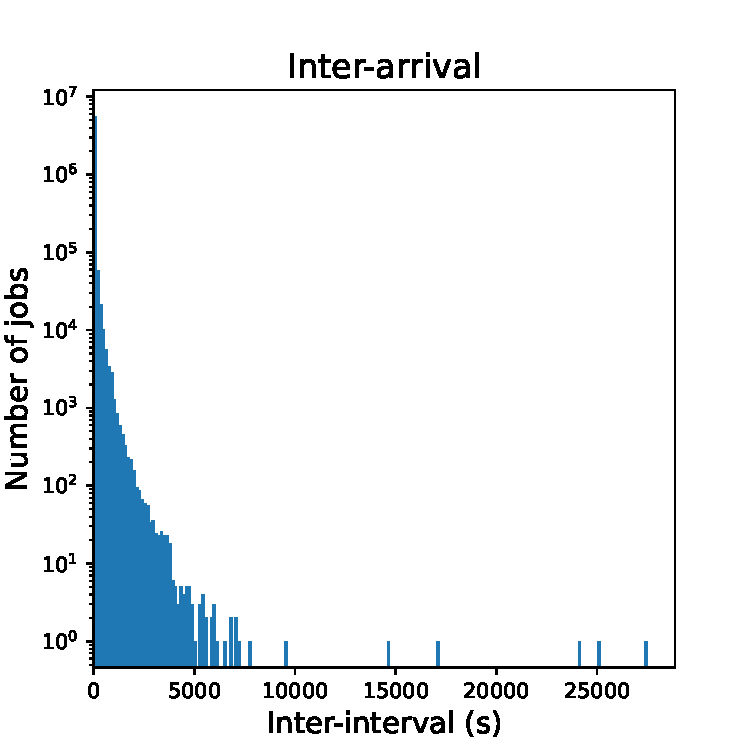
\includegraphics[scale=0.55]{Images/Model/interarrival.pdf}
    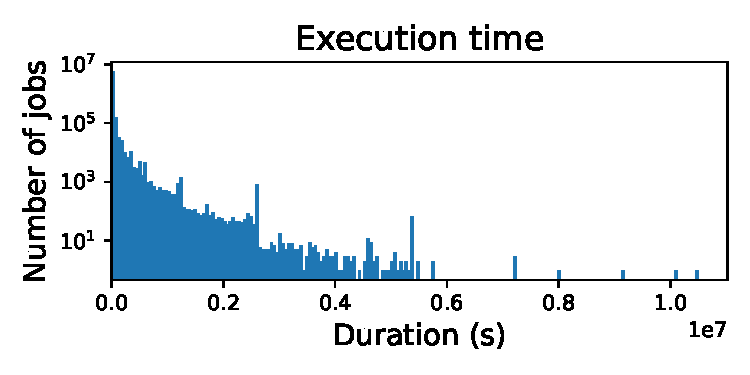
\includegraphics[scale=0.55]{Images/Model/execution_time.pdf}
    \caption{Inter arrival and execution time distribution for MetaCentrum2 workload trace.}
    \label{fig:metacentrum}
\end{figure}

Another aspect of the MetaCentrum2 workload is the \textit{Requested Time} field. This field could be considered as walltime. Nevertheless, MetaCentrum2 defines this field according to the job queue. Consequently, it does not come from the user. We recalculate the walltime using the proposition from \citeauthor{takizawa2020effect} \cite{takizawa2020effect}. Thus, we equally divided the jobs into five groups. Each group estimates the walltime as follows:

\begin{enumerate}
    \item walltime = real execution time $\times$ 5
    \item walltime = real execution time $\times$ 3.333333333
    \item walltime = real execution time $\times$ 2
    \item walltime = real execution time $\times$ 1.428571429
    \item walltime = real execution time $\times$ 1.111111111
\end{enumerate}

This uncertainty complicates the scheduling decisions but it is more realistic. We created two scripts for translating the SWF format to the simulator chosen (see Section \ref{sec:BATSIM}) and Datazero2 Middleware formats. We simulated several possibilities of workload, and each chapter will describe the selection process.

\subsection{Weather Trace}
\label{sec:weather_trace}

Regarding weather, we are interested in the traces of solar irradiance and wind speed, which allow us to estimate power generation using Equations \ref{equ:panel_solar_with_temperature} and \ref{equ:wind_turbines}. NASA's Modern-Era Retrospective Analysis for Research and Applications (MERRA) provides a dataset of solar irradiance and wind speed from any place in the world \cite{rienecker2011merra}. Regarding wind speed, we get the data directly from the MERRA site\footnote{https://power.larc.nasa.gov/data-access-viewer/}. Renewable Ninja\footnote{https://www.renewables.ninja/} is a tool that transforms the weather from MERRA to electricity production \cite{pfenninger2016long, staffell2016using}. Renewable Ninja uses some solar panel models to estimate power generation. We use Renewable Ninja to obtain ground-level solar irradiance because the authors consider cloud cover and aerosols' impact on the irradiance. We chose Toulouse, France as the reference point, getting the data from 2020. After exporting the data, we also translate the output CSV to the simulator chosen (see Section \ref{sec:BATSIM}) and Datazero2 Middleware formats. We took different days from 2020 for our simulations. The following chapters will present the selection process.

\subsection{Platform Configuration}
\label{sec:platform_configuration}

Finally, the last data is the hardware specification. This configuration simulates the real behavior of the different components of a data center, such as servers, storage, network, etc. In this thesis, we focused on the server specification. For simulating a DVFS-enabled server, the following information is necessary:
\begin{itemize}
    \item Sleeping power: Power used to maintain a server sleeping;
    \item Time for on\(\rightarrow\)off transition: Time to turn off a server;
    \item Power for on\(\rightarrow\)off transition: Power to turn off a server;
    \item Time for off\(\rightarrow\)on transition: Time to turn on a server;
    \item Power for off\(\rightarrow\)on transition: Power to turn on a server;
    \item Power idle: Power used when the server is idle;
    \item DVFS states: A list of states containing:
    \begin{itemize}
        \item Power: The power used in the state with all processors busy;
        \item Speed: The speed in the state.
    \end{itemize}
\end{itemize}

We chose to model a data center using the specification from GRID5000 servers. \citeauthor{dacosta:hal-03453537v1} performed experiments in GRID5000 to obtain the data for the DVFS states \cite{dacosta:hal-03453537v1, dacostakeynote}. Some other authors also simulated GRID5000 machines, giving information about their simulation \cite{rais2018quantifying, caux2018optimization, caux2019phase, villebonnet2016energy}. We consolidate these works to create a platform for both the simulator chosen (see Section \ref{sec:BATSIM}) and Datazero2 Middleware. Table \ref{tab:gros} exemplifies the consolidated data for GRID5000's Gros server used in the experiments.

% \begin{table}[!htb]
% \centering
% \caption{Gros definition. The power is for all server's processors busy. The values are from Grid5000's Gros server.}
% \label{tab:gros}
% \begin{tabular}{ll|l}
%     \hline
%     \multicolumn{2}{l|}{Parameter} & Value \\ \hline\hline
%     \multicolumn{2}{l|}{Sleeping power} & 4.5 W \\
%     \multicolumn{2}{l|}{Time on-\textgreater{}off} & 6 s \\
%     \multicolumn{2}{l|}{Power on-\textgreater{}off} & 76.5 W \\
%     \multicolumn{2}{l|}{Time off-\textgreater{}on} & 164 s \\
%     \multicolumn{2}{l|}{Power off-\textgreater{}on} & 110.52 W \\
%     \multicolumn{2}{l|}{Power idle} & 62 W \\ \hline
%     \multicolumn{3}{l}{DVFS states}  \\ \hline 
%     \multicolumn{1}{l|}{State} & Power (W) & Speed per core (Gflops) \\ \hline\hline
%     \multicolumn{1}{l|}{0} & 143.45 & 35.2 \\
%     \multicolumn{1}{l|}{1} & 123.57 & 33.59 \\
%     \multicolumn{1}{l|}{2} & 122.34 & 31.98 \\
%     \multicolumn{1}{l|}{3} & 121.68 & 30.36 \\
%     \multicolumn{1}{l|}{4} & 118.49 & 28.79 \\
%     \multicolumn{1}{l|}{5} & 115.8 & 27.14 \\
%     \multicolumn{1}{l|}{6} & 114.58 & 25.57 \\
%     \multicolumn{1}{l|}{7} & 110.89 & 23.85 \\
%     \multicolumn{1}{l|}{8} & 108.06 & 22.38 \\
%     \multicolumn{1}{l|}{9} & 106.81 & 20.78 \\
%     \multicolumn{1}{l|}{10} & 104.13 & 19.18 \\
%     \multicolumn{1}{l|}{11} & 102.83 & 17.59 \\
%     \multicolumn{1}{l|}{12} & 100.78 & 15.99 \\ \hline
% \end{tabular}
% \end{table}

\begin{table}[!htb]
    \caption[Gros definition]{Gros definition. The power is for all server's processors busy. The values are from Grid5000's Gros server.}
    \label{tab:gros}
    \begin{minipage}{.45\linewidth}
      \centering
      \begin{tabular}{l|l}
        \hline
        Parameter & Value \\ \hline\hline
        Sleeping power & 4.5 W \\
        Time on$\rightarrow$off & 6 s \\
        Power on$\rightarrow$off & 76.5 W \\
        Time off$\rightarrow$on & 164 s \\
        Power off$\rightarrow$on & 110.52 W \\
        Power idle & 62 W \\ \hline
    \end{tabular}
    \end{minipage}%
    \begin{minipage}{.55\linewidth}
      \centering
      \begin{tabular}{l|l|l}
        \hline
        State & Power (W) & Speed per core (Gflops) \\ \hline\hline
        0 & 143.45 & 35.2 \\
        1 & 123.57 & 33.59 \\
        2 & 122.34 & 31.98 \\
        3 & 121.68 & 30.36 \\
        4 & 118.49 & 28.79 \\
        5 & 115.8 & 27.14 \\
        6 & 114.58 & 25.57 \\
        7 & 110.89 & 23.85 \\
        8 & 108.06 & 22.38 \\
        9 & 106.81 & 20.78 \\
        10 & 104.13 & 19.18 \\
        11 & 102.83 & 17.59 \\
        12 & 100.78 & 15.99 \\ \hline
    \end{tabular}
    \end{minipage} 
\end{table}

\section{Simulation}
\label{sec:simulation}

After describing the source of data, we detail our simulation environment. We explain two simulators and the work done to adapt our data for these simulators. We define the different metrics used to evaluate the algorithms in the following chapters.

\subsection{Batsim Simulator}
\label{sec:BATSIM}

Batsim is an infrastructure simulator that enables the study of resource management policies \cite{batsim_jsspp16}. This simulator is based on the well-known Simgrid \cite{casanova2001Simgrid}. The Batsim protocol helps to develop scheduling and resource management algorithms without Simgrid knowledge. The protocol works via a socket and includes the following events:
\begin{itemize}
    \item Bidirectional (Batsim$\rightarrow$Scheduler and Scheduler$\rightarrow$Batsim):
    \begin{itemize}
        \item \textit{QUERY}: It has two queries. First, in the \textit{consumed\_energy} query, the scheduler asks Batsim about the total consumed energy (from time 0 to now). On the other hand, in the \textit{estimate\_waiting\_time}, Batsim demands the scheduler what would be the waiting time of a potential job;
        \item \textit{ANSWER}: The \textit{QUERY} answer;
        \item \textit{NOTIFY}: This event allows a peer to notify something to its counterpart. This message can be a specific message from an external event.
    \end{itemize}
    \item Batsim$\rightarrow$Scheduler:
    \begin{itemize}
        \item \textit{JOB\_SUBMITTED}: A new job was submitted;
        \item \textit{JOB\_COMPLETED}: The job has completed its execution;
        \item \textit{JOB\_KILLED}: The job was killed;
        \item \textit{RESOURCE\_STATE\_CHANGED}: The state of a resource (server) changed;
    \end{itemize}
    \item Scheduler$\rightarrow$Batsim:
    \begin{itemize}
        \item \textit{EXECUTE\_JOB}: Execute the job in the servers;
        \item \textit{KILL\_JOB}: Kill the running job;
        \item \textit{SET\_RESOURCE\_STATE}: Set the state of a resource (server);
    \end{itemize}
\end{itemize}

These are some messages of the protocol (the entire protocol is in Batsim documentation\footnote{https://batsim.readthedocs.io/en/latest/protocol.html}). The messages \textit{QUERY} and \textit{ANSWER} enable the scheduler to receive IT energy consumption. The scheduler uses the \textit{JOB\_SUBMITTED}, \textit{JOB\_COMPLETED}, \textit{JOB\_KILLED}, \textit{EXECUTE\_JOB}, and \textit{KILL\_JOB} messages to control the jobs. Finally, the \textit{SET\_RESOURCE\_STATE} and \textit{RESOURCE\_STATE\_CHANGED} allow server configuration. However, Batsim does not provide the electrical management of renewable sources and energy storage. Considering renewable sources, the main objective is receiving power production. Therefore, we applied Equations \ref{equ:wind_turbines} and \ref{equ:panel_solar_with_temperature} on the data from Section \ref{sec:weather_trace}, resulting in a time series of power production. Then, we create a file with several JSON lines:

\begin{lstlisting}[language=json,firstnumber=1]
    {"type": "user_specific_type", "timestamp": 0, "power_available": 0.0}
    {"type": "user_specific_type", "timestamp": 300, "power_available": 460.4}
    {"type": "user_specific_type", "timestamp": 600, "power_available": 5172.26}
\end{lstlisting}

Batsim reads this file and sends at each "timestamp" a \textit{NOTIFY} message. Then, we parse the JSON in the message, taking the power available. $\Delta t$ defines the interval between messages. The scheduler does not know all the events in this JSON file, receiving them just when the simulation arrives at the "timestamp". Regarding energy storage, we implemented two classes to simulate them. The first class is for the battery and uses Equations \ref{equ:battery_energy} and \ref{equ:battery_state_of_charge} to estimate the state of charge. The second class is for hydrogen and implements Equations \ref{equ:hydrogen_electrolyzer}, \ref{equ:hydrogen_full_cell}, and \ref{equ:hydrogen_level}. The energy storage implementation must respect the following constraint:

\begin{equation}
    \label{equ:energy_diff}
    ((P_{renew} + P_{dch} + P_{fc} - P_{ez} - P_{ch}) \times \Delta t \times 1000) - E_{tot} = 0
\end{equation}

Constraint \ref{equ:energy_diff} indicates that the difference between energy production ($(P_{renew} + P_{dch} + P_{fc} - P_{ez} - P_{ch}) \times \Delta t \times 1000$) and the energy expended by the IT ($E_{tot}$) must be equal to zero. $P_{renew}$ comes from the JSON input with no modifications. $E_{tot}$ is calculated using \textit{QUERY} and \textit{ANSWER} messages. Since it returns the total energy expended (from 0 to now), we calculate the difference between two \textit{QUERY} calls. So, the simulator balances $P_{dch}$,  $P_{fc}$, $P_{ez}$, and $P_{ch}$. In the default implementation, the simulator first adapts the battery ($P_{dch}$ and $P_{ch}$), and, just if necessary, it changes the hydrogen ($P_{fc}$ and $P_{ez}$).  However, it depends on the implementation (e.g., if the offline plan indicates something different). This simulation respects the boundaries \ref{equ:discharge_boundary}, \ref{equ:charge_boundary}, \ref{equ:fuelcells_boundary}, and \ref{equ:electrolyzer_boundary}.

Another input for Batsim is the platform file. Batsim uses the Simgrid platform format\footnote{https://simgrid.org/doc/latest/Platform.html}. Using the results from Section \ref{sec:platform_configuration}, we created a script to generate this file with all DVFS states. This script receives the server parameters (e.g., Table \ref{tab:gros}) and the number of nodes from this server. It can create homogeneous and heterogeneous data centers according to the user specification. Finally, the last input for Batsim is the workload file. Batsim simplifies the workload definition of HPC jobs. We focused on the Homogeneous Parallel Task kind of application in the experiments. In this application type, we define the amount of floating-point operations (flops) to execute on each machine. Here, we create another script to translate the SWF format (from Section \ref{sec:workload_trace}) to Batsim JSON format. An example of a workload file is:

\begin{lstlisting}[language=json,firstnumber=1]
{
    "jobs": [
        {
            "id": "0",
            "profile": "profile_1",
            "res": 1,
            "subtime": 773,
            "walltime": 9112
        }
    ],
    "profiles": {
        "profile_1": {
            "cpu": 163137000000000,
            "type": "parallel_homogeneous"
        }
    },
}       
\end{lstlisting}

In this example, we have only one job with the id equal to 0. This job is submitted after 773 seconds from the simulation beginning (\textit{"subtime": 773}), with a walltime of 9112 seconds (\textit{"walltime": 9112}), and requests one machine (\textit{"res": 1}). The scheduler only knows these fields. The profile field indicates the number of flops to execute. Therefore, the job must calculate 163137000000000 flops. The real execution time is \textit{cpu} divided by the speed of the server which runs this job. The script estimates the field \textit{cpu} by the execution time in SWF multiplied by a server's average speed. We defined the average speed considering the servers in our data center. We took a median DVFS state's speed, avoiding over/underestimating. This estimation is necessary because SWF does not provide any metric of the real computation. All experiments in this thesis use Batsim as the simulator. In parallel, we implement our algorithms in Datazero2 Middleware.

\subsection{Datazero2 Middleware}

The Datazero2 project proposes a middleware to integrate all components from Figure \ref{fig:model}. This middleware has all electrical and IT components, external event integrations, and decision modules. It works on two coding languages: Python and C++. It depends on different frameworks, such as:
\begin{itemize}
    \item ActiveMQ 5.14.4;
    \item C++:
    \begin{itemize}
        \item Protobuf 3.21.8;
        \item Apache APR 1.7.4;
        \item ActiveMQ C++ library 3.9.5;
        \item Simgrid 3.27;
    \end{itemize}
    \item Python:
    \begin{itemize}
        \item Stomp 8.1
        \item Protobuf 3.20.3
        \item Pandas
        \item Pulp
    \end{itemize}
\end{itemize}

Some modules work in Python, and some in C++. The messages from the modules are exchanged via ActiveMQ, using Protobuf as protocol. Simgrid is used to simulate the IT side. The electrical side is implemented using the same rules presented in this thesis. This middleware is still in development by different actors in the project. During this thesis, we worked on the ODM implementation. The results from the Batsim simulations are being implemented in the middleware. 

However, we helped with all these dependencies management, allowing every project's partner to execute the middleware on their computers. Therefore, we create a docker version of the middleware. We create three containers: ActiveMQ, C++, and Python. The ActiveMQ provides the message BUS for all the modules. C++ implements the Simgrid and some modules (e.g., ODM). Python has the electrical control and other modules (e.g., ITDM and PDM). We create a docker-compose script that installs and compiles everything. We included some advanced parameters for developers for coding inside docker without the need to rebuild everything.

Regarding the middleware's simulation input, some changes were done. The weather data is passed directly to the middleware, which applies the equations to transform weather into power. Even if it uses Simgrid (so, same platform file format), the middleware divides this file into two files: Model and Machines. The Model file defines the DVFS states, including a model id. The Machine file indicates all the servers, linking each one to a model id. This division simplifies the modifications in the model. So, we create a new version of the platform script, allowing choose between Batsim or Datazero2 middleware. Finally, the workload file is not JSON but XML. We also create a new version of our script to migrate from SWF to Datazero2 middleware XML.

\subsection{Metrics}

In this section, we present the metrics used in this thesis. We evaluate four aspects in this thesis: Jobs finished, storage state at the end of the time window, wasted energy, and bounded slowdown. The first objective is to increase the number of finished jobs and reduce the number of killed jobs. It is possible to have a high number of finished jobs and a high number of killed jobs in aggressive scheduling, where the scheduler starts jobs even if it is not possible to finish them. Each job can finish in one of five states: 

\begin{enumerate}
    \item Finished: Jobs that finished their computation before the walltime;
    \item Postponed: Jobs postponed to the next time window;
    \item Reached walltime: The jobs that reached the walltime because they do not finish all the computation due to the servers speed;
    \item Not completely finished: The jobs that were not finished completely because they are still running at the end of the time window;
    \item Killed: The killed jobs.
\end{enumerate} 

Therefore, we present the absolute number of jobs in each state at the end of the simulation. In addition, we introduce this metric considering the size of the job ($Dfl_j \times R_j$). The size of the job shows the impact of the decisions in bigger and small jobs. The second aspect is the algorithms must end the time window with the storage levels as close as possible to the planned. This means the algorithms can not "cheat" by using more storage than planned. As explained before, finishing close to the target levels helps to plan the next time window. We present a metric of the distance from the target. This distance can be positive (save more energy) or negative (use more energy). For battery, we present it as the \% difference of target SoC, and for hydrogen, we present it as the kg difference of target LoH.

The third metric is wasted energy. We consider wasted energy the energy expended not computing finished jobs, englobing, for example, the energy used in killed jobs, turning on/off servers, and letting servers idle. This metric is present as kWh. Finally, the fourth metric is the bounded slowdown. This metric is the same as presented in Equation \ref{equ:slowdown}. The bounded slowdown is a difficult metric to compare in executions without the same number of jobs finished. For example, starting and killing a job in the sequence will result in a very low slowdown. On the other hand, maintaining jobs running will make the jobs in the queue wait for more time, which impacts directly on the slowdown. So, we will analyze this metric with precaution.

\section{Conclusion}
This chapter focused on presenting the model, data, and simulation utilized in the remainder of this thesis. The aim is to provide the basis to understand the following chapters. The model introduces all aspects of offline decisions. This offline module builds a plan for the online module. The online model considers the offline as a guide but improves this plan according to the real events. Moreover, the online model considers job scheduling in the decision process. Then, we describe the work done in the data for the simulations. This work includes workload, weather, and platform information. Finally, we explained simulation tools. We detailed the modifications in Batsim to use renewable energy and energy storage. Moreover, we present the metrics used in this thesis to compare the different approaches.

The next chapter introduces the first heuristic to deal with power compensations, trying to improve QoS. After that, Chapter \ref{cha:learning_power_compensations} proposes a model for learning the best power compensations. Finally, Chapter \ref{cha:heuristic} presents our final heuristic, using predictions to make better decisions.

    \chapter{Introducing Power Compensations}
\label{cha:power_compensations}

\minitoc

\section{Introduction}

In this chapter, we propose some heuristics to solve the problem from the model presented in Section \ref{sec:ODM}. The main objective is to adapt the offline plan according to real power production and usage. First, we describe the heuristics to solve it, linking with the model from Chapter \ref{cha:model}. Then, we explain the experimental environment used in the experiments. Finally, we present and discuss the results, highlighting the impact of the power constraints.

\section{Proposed Approach}

We divided the heuristic into two parts. First, we detail the scheduling decisions. The scheduler defines the job priority and placement. Also, the scheduler tries to avoid killing jobs, demanding more power if needed. Then, we describe the power compensation heuristics. These heuristics approximate the battery's state of charge from the target level.

\subsection{Scheduling}
\label{sec:heuristic_scheduling}

Job scheduling is a well-known problem NP-complete problem \cite{robert2009introduction, agrawal2021energy}. Several heuristics are proposed to solve this problem in an acceptable time. We implemented a well-known algorithm named EASY Backfilling in this chapter \cite{mu2001utilization}. This heuristic is known for its simple and robust implementation \cite{srinivasan2002characterization}. Also, it maximizes server utilization \cite{srinivasan2002characterization}. This algorithm englobes queue sorting and placement. First, it places priority jobs in the available servers. Then, it fills the scheduling holes with small jobs (see Figure \ref{fig:backfilling}). Algorithm \ref{alg:algo_scheduling} denotes a pseudo-code of EASY Backfilling, presented by \citeauthor{lelong2018tuning} as EASY-$P_{R}$-$P_{B}$ policy \cite{lelong2018tuning}. ODM uses this heuristic when a job arrives, a job finishes or new servers are available. 

\IncMargin{1em}
\begin{algorithm}[!htb]
    \LinesNumbered
    \footnotesize
    \SetAlgoLined
    \SetKwInOut{Input}{input}\SetKwInOut{Output}{output}
    \Input{Queue $Q$ of waiting jobs, $P_{R}$ as priority order, and $P_{B}$ as backfilling order.}
    \Output{None (calls to \textit{Start()})}
    \Begin{
        Sort $Q$ according to $P_{R}$\;
        \For{job $j$ in $Q$}{
            Pop $j$ from $Q$\;
            $S_j \leftarrow$ \textit{select\_servers($j$)}\;
            \uIf{$j$ can be started in servers $S_j$}{
                \textit{Start($j$, $S_j$)}\;
            }\Else{
                Reserve $j$ at the earliest time possible according to the walltime of the currently running jobs\;
                Sort $Q$ according to $P_{B}$\;
                \For{job $j^{'}$ in $Q$}{
                    $S_j \leftarrow$ \textit{select\_servers($j^{'}$)}\;
                    \If{$j^{'}$ can be started in servers $S_j$ without delaying the reservation on $j$}{
                        \textit{Start($j^{'}$, $S_j$)}\;
                    }
                }
                \textbf{break}\;
            }
        }
    }
    \caption{EASY-$P_{R}$-$P_{B}$ scheduling \cite{lelong2018tuning}.}
    \label{alg:algo_scheduling}
\end{algorithm}
\DecMargin{1em}

First, this heuristic sorts the jobs in the queue in a priority order $P_{R}$ (line 2). Then, it selects the servers to run this job (line 5). If the job $j$ can start in the servers $S_j$ (line 6), it places the job in the servers (line 7). When it finds a job that can not be placed now, it starts to backfill (lines 9-17). Then, it reserves the first moment to run this job (named priority job) in the future (line 9). So, it re-sorts the queue using $P_{B}$ (line 10), placing the other jobs in the servers (lines 11-16) without delaying the (future) priority job execution (line 13). As presented, the algorithm sorts the queue using $P_{R}$ (in the priority moment) and $P_{B}$ (in the backfilling moment). However, the typical implementation uses the same sort for both \cite{lelong2018tuning}. Our first implementation uses the typical algorithm (same sorting policy), but Chapter \ref{cha:heuristic} uses two policies. Thus, $P_{R}$ and $P_{B}$ apply Descending Bounded Slowdown (higher Bounded Slowdown first) policy from Equation \ref{equ:slowdown}. This order helps to let a job wait proportionately to its size.

Besides the placement, the scheduler maintains the jobs running at least at a "minimal speed". This minimal speed is given by Equation \ref{equ:avoid_walltime}. The idea is to keep the jobs' servers at the speed $D_{s,d}$. For example, if $D_{s,d}$ is too slow, the job can reach the walltime without finishing all its computing. Also, if the offline plan indicates to sedate a server, the jobs running on this server are killed. So, every time step $t$, the scheduler verifies the energy needed to maintain the jobs running at least at the minimal speed. If it is necessary to use more energy now (changing the plan), it verifies if it is possible to migrate power from the future to now. This verification consists of two tests:
\begin{enumerate}
    % \item \textit{Does the battery have the energy to be migrated?} The algorithm calculates how much battery energy is planned to be used in the future. The algorithm must let minimal energy to maintain all servers in the sleep state (it can come from battery, renewable, or hydrogen). So, the energy needed to maintain jobs running must be present in the sum of future usage;
    % In this test, the algorithm verifies the battery usage in future steps. Let $P_{min}$ be the power needed to maintain all servers in the sleeping state. So, for each step, the energy possible to migrate from the batteries is equal to:
    % \begin{itemize}
        %     \item If $P_{fc} > P_{min}$: $P_{renew} + P_{dch} - P_{ch}$. In this case, hydrogen maintains the servers in the sleeping state. So all renewable can be used to charge the battery;
        %     \item If not: $P_{renew} + P_{dch} - P_{ch} - P_{ez} - P_{min}$
        % \end{itemize}
    \item \textit{Will battery boundaries be violated?} Equation \ref{equ:battery_boundaries} must be respected. So, migration can not violate the SoC boundaries;
    \item \textit{Is it possible to compensate for this change?} This verification is explained in Section \ref{sec:power_compensation};
\end{enumerate}

If possible, the scheduler modifies the offline IT plan to let the servers run at the speed $D_{s,d}$. If it is not possible, the scheduler does not change the offline plan. 

\subsection{Power compensations}
\label{sec:power_compensation}

After describing the scheduling algorithm, this section explains the heuristic to compensate for power fluctuations presented in Section \ref{sec:ODM}. The objective of power compensations is to ensure that $SoC$ and $LoH$ are close to the offline plan at the end of the time window. Therefore, every time step $t$, ODM calculates $E_{comp}$ using Equation \ref{equ:energy_battery}. $E_{comp}$ can be positive or negative, according to battery usage or renewable production. Thus, the problem is to define the future time step to change power usage to use the energy $E_{comp}$. Let $t'$ be the future time step. Then, ODM must change $P_{dch}(t')$ and $P_{ch}(t')$. Of course, $P_{dch}$ and $P_{ch}$ are power, and $E_{comp}$ is energy, so we make the conversion from power to energy in this process. Also, the changes must consider the boundaries from Equations \ref{equ:discharge_boundary} and \ref{equ:charge_boundary}. In addition, even if all servers are sleeping, minimal power must be delivered since the power usage in the sleep state is not zero. Let $P_{min}$ be the minimal power possible. Then, $P_{prod}(t') \ge P_{min}$, considering that $P_{prod}$ comes from Equation \ref{equ:model_energy}. Nevertheless, the compensation still considers the estimated renewable production from the future steps.

ODM spreads the energy over different $t'$ until all modifications compensate for $E_{comp}$. The power compensations happen in two cases:
\begin{enumerate}
    \item Every time step, ODM recalculates $SoC(T)$ using Equation \ref{equ:battery_energy} from the actual step until $T$. Then, it compares $SoC(T)$ and $SoC_{target}$, using Equation \ref{equ:delta_energy}. Finally, ODM compensates $E_{comp}$ (from Equation \ref{equ:energy_battery}), approximating $SoC(T)$ to $SoC_{target}$ (respecting Equation \ref{equ:soc_target});
    \item When the scheduler demands more power, as presented in Section \ref{sec:heuristic_scheduling}, it tries to maintain the servers with jobs running. So, it increases the power usage at the step. This increase will change the $SoC(T)$, demanding compensation. This compensation is always negative (if ODM uses more power now, it needs to use less in the future).
\end{enumerate}

If ODM can not entirely compensate $E_{comp}$, it has two possible actions. If the request for compensation comes from the scheduler (case 2), it does not make the modifications demanded by the scheduler, impacting the jobs. On the other hand, in case 1, ODM will modify as much as possible. On Datazero2, the impossibility of compensating for case 1 can start a new negotiation from the offline part to deal with this event. However, in this thesis we let the ODM run to see the impact of these cases.

The question now is: in which future time step $t'$? To answer this, we propose four policies: \emph{Peak}, \emph{Next}, \emph{Last}, and \emph{Load}. Figure \ref{fig:compensation} illustrates an example of these policies. The \emph{Next} and \emph{Last} policies execute the same search independently of the type of compensation (positive or negative compensation). While the \emph{Next} policy takes the $t + 1$, \emph{Last} policy takes $T$. On the other hand, \emph{Peak} and \emph{Load} take different steps according to the compensation (positive or negative). \emph{Peak} policy finds the higher power production ($P_{prod}$) peak in negative compensation and the lower peak in positive compensation. This policy will "shave" the peaks, tending to a flat curve. \emph{Load} policy considers the different between demand ($P_{load}$) and production ($P_{prod}$). In positive compensation, this policy takes the higher difference $P_{load} - P_{prod}$, while in negative it takes the smaller one. In Figure \ref{fig:compensation}, if the scheduler saves energy at step 1, it could compensate for it at step 3 (\emph{Next}), step 12 (\emph{Peak}), step 15 (\emph{Last}), or step 14 (\emph{Load}). Even if Figure \ref{fig:compensation} compensates only one time, the algorithm can select more than one until compensate $E_{comp}$ entirely and follows its policy (e.g., Next will take step 2, 3, 4, etc.).

\begin{figure}[!htb]
    \centering
    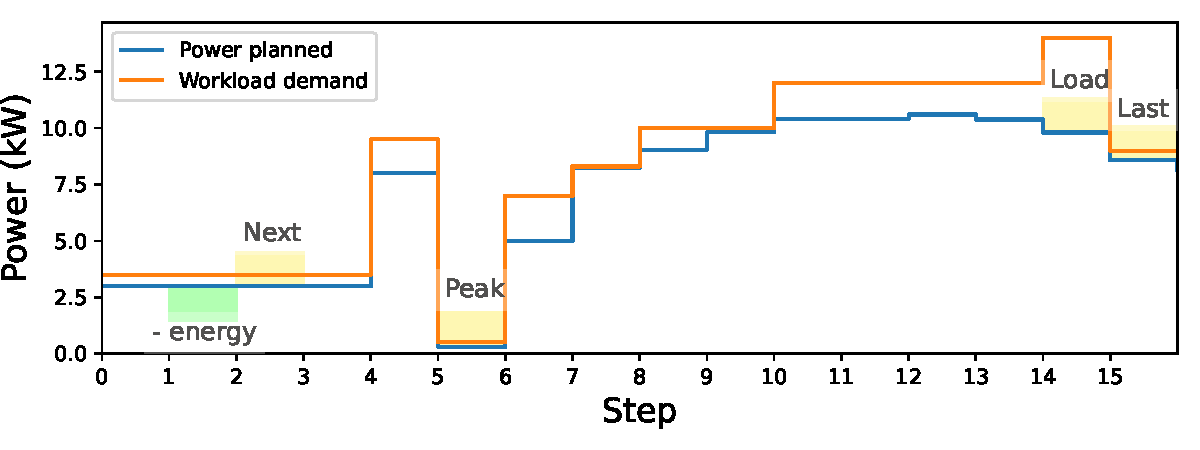
\includegraphics[scale=0.7]{Images/Compensations/policies.pdf}
    \caption{Compensation policies. The blue curve is the offline usage plan ($P_{prod}$) and the orange line is the estimated demand ($P_{load}$). In this example, it saves some energy in time step 1 (see the green square). So, it can reintroduce this energy in future time steps (see the yellow squares).}
    \label{fig:compensation}
\end{figure}

Finally, the last part of the heuristic is transforming the power modifications into server configuration. Since the IT offline plan gives the P-state of the servers for each step $t$, we must adapt this plan for the new power. We propose a heuristic to find quick solutions. The four policies use the same heuristic to distribute the compensation. This heuristic has a list of all power and speed differences between two P-states, so it can fastly decide which one will impact the most on data center speed. First, it calculates the difference between the power usage in the offline plan and the power to use. If this difference is positive, it can improve the server configuration, speeding up or turning on servers. It goes through the list searching for the highest flops improvement below or equal to the power increment. It does it in the following order:
\begin{enumerate}
    \item Find the highest improvement possible for the servers running some job;
    \item Find the highest improvement possible for the idle servers.
\end{enumerate}

Taking Table~\ref{tab:gros} as an example, let's say that we have two servers running jobs: one on state 5 and another on state 10. If the system has 30 W to increase, it will increase first the server on state 10 to state 1, because it will increase 14.41 Gflops (against 6.45 Gflops from state 5 to state 1). If a server is sleeping, it also considers the power needed to turn the server on. When the difference between offline and online power is negative, the algorithm must reduce the speed of the servers. So, it does the following:
\begin{enumerate}
    \item Reduce the speed of idle servers;
    \item Reduce the speed of the servers running jobs. We calculate $(wall_{j} - elapTime_{j})$ for each job. Then, we sort the servers by this value in decreasing order.
\end{enumerate}

It stops after the first modification which let the power usage lower or equal to the power production $P_{prod}(t)$. The second step will reduce servers' speed with more time to compensate for this reduction in the future. It is better to maintain jobs closer to finish with the maximum speed, granting that they will complete.

\section{Experimental environment}
\label{sec:experiment_environment}
% IT (servers)
% Electrical (battery, solar, wind, etc)
% Workload Trace
% Weather Trace

In this section, we present the environment used to run our simulations. This environment englobes IT servers definition, electrical elements, and the workload and weather traces. We focus on simulating a time window of three days ($T_{w}=259200 s$), divided into time steps of 5 minutes ($\Delta t=300$). We chose time steps of 5 minutes because it is neither too long to react to events nor too short for server transitions. For example, a time step of 1 minute is good for adapting the battery usage, but it is not enough to turn on a server (Table \ref{tab:gros} shows that a Gros server takes 164 seconds to finish the off$\rightarrow$on transition). A longer time step can be too late to adapt battery usage. Regarding the server specification, we simulated a homogeneous data center using the GRID5000's Gros server. Their parameters were presented in Table \ref{tab:gros}. We present the experiments in a homogeneous data center to ease the understanding. However, we present different experiments in a heterogeneous data center in \cite{de2022analyzing}. Our data center is composed of 400 servers with Gros specifications. Other aspects, such as network and memory are ignored. 

Considering the electrical components, the data center is composed of solar panels, wind turbines, batteries, and one hydrogen tank. The total size of the batteries is 800 kWh ($B_{size}=800kWh$). The efficiency of charging is 0.82 ($\eta_{ch}=0.82$) and discharging is 1.22 ($\eta_{dch}=1.22$). We defined the thresholds $SoC_{min}$ and $SoC_{max}$ as 20\% and 90\%. So, the range of available energy from the battery allows to run the whole data center for 9.76 hours. We set the max charge and discharge power as 80\% of the battery size ($P_{ch_{max}}=640kW$ and $P_{dch_{max}}=640kW$). The hydrogen tank has 20000 kg ($LoH_{max}=20000$), with the electrolyzer's efficiency of 97.5 and the fuel cell's efficiency of 13.332. We defined that the battery starts half charged ($SoC(0)=50\%$) and the hydrogen with 300 kg ($LoH(0)=300kg$). We defined also that they should come back at least to the same value as they started at the end of the time window ($SoC_{target} = 50\%$ and $LoH_{target}=300kg$).

Regarding workload and weather traces, we have divided the experiments into two parts. The first part aims to analyze the decisions in critical scenarios (named \emph{critical scenarios}) and the second part focuses on the average cases (named \emph{average scenarios}). 

\subsection{Critical Scenarios}

In the first part, we have taken two workloads from the Metracentrum dataset with the size of three days. One of them has jobs arriving mainly on the first day, and the second one has jobs arriving mainly on the third day. Figure \ref{fig:critical_workload} illustrates the demanded power of both workloads. The demanded power is calculated using 400 Gros servers without power constraints (e.g., the servers are available all the time). The first workload has 3729 jobs and the second workload has 3158 jobs. 

\begin{figure}[!htb]
    \centering
    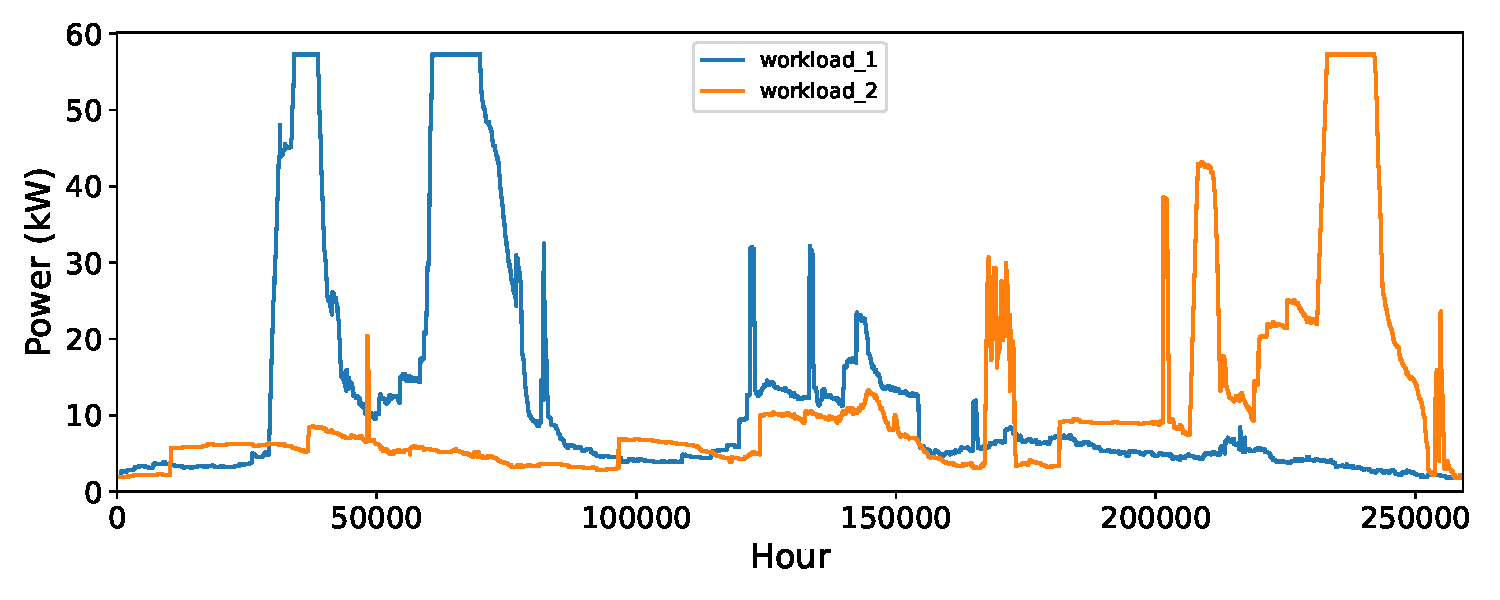
\includegraphics[scale=0.58]{Images/Compensations/critical_jobs_arriving.pdf}
    \caption{The power demanded for the critical scenarios.}
    \label{fig:critical_workload}
\end{figure}

We generated the weather data using MERRA and renewable ninja of 3 days for the \emph{critical scenarios}. Figure \ref{fig:critical_weather} shows the power production generated by the weather using the electrical components of our data center. 

\begin{figure}[!htb]
    \centering
    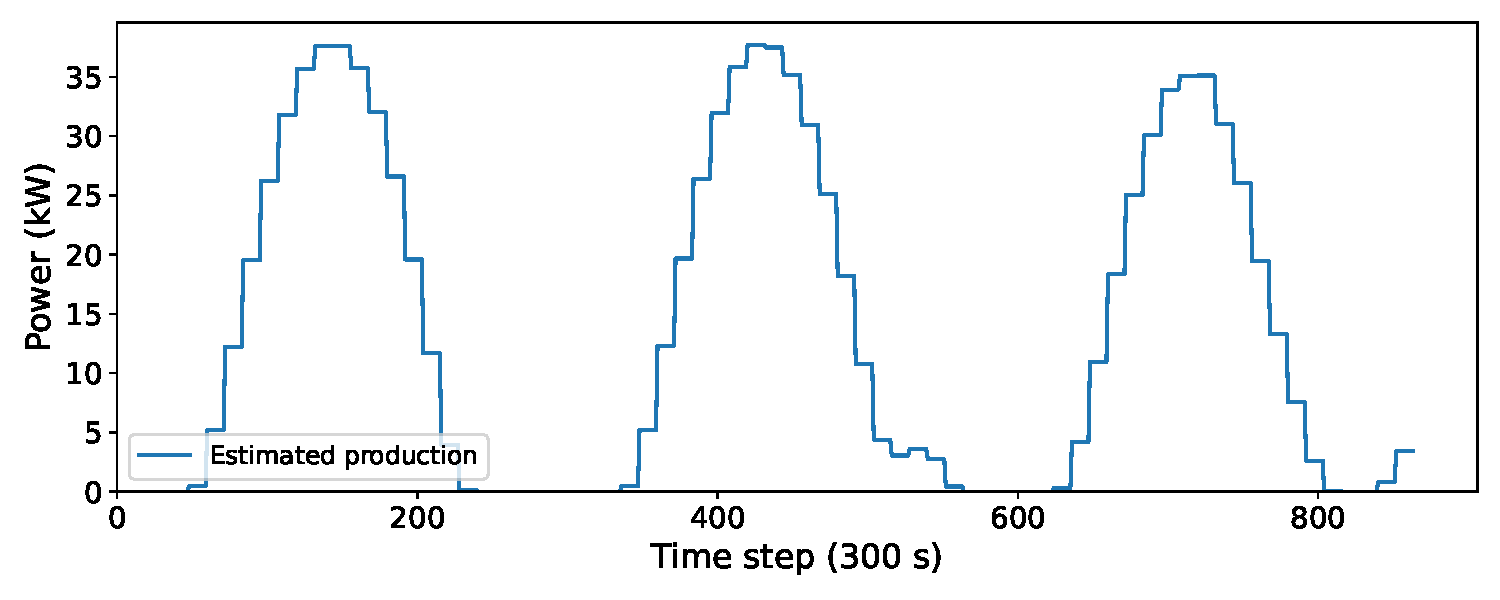
\includegraphics[scale=0.58]{Images/Compensations/critical_power_production.pdf}
    \caption{The power production for the critical scenarios.}
    \label{fig:critical_weather}
\end{figure}

We consider both workload and weather as predictions. Then, we use them to create an offline plan as presented in Section \ref{sec:offline_plan}. First, we solved the PDM model from Section \ref{sec:offline_modules} using the linearization proposed by \citeauthor{haddad2019mixed} \cite{haddad2019mixed}. Then, we took the production ($P_{prod}$) and solved the ITDM model. The ITDM model presented in Section \ref{sec:offline_modules} is too complex to solve a three-day time window with 400 servers. So, we simplified the problem, ignoring the transitions on$\rightarrow$off and off$\rightarrow$on. This new model returns the number of servers on and off at each time step and can be solved faster. After that, we have the offline plan. 

The next step is to introduce noise in the predictions to emulate the variations in reality. Every prediction provides a range of where the forecast is likely to be. So, we generated noises inside this range. In the critical scenarios, we considered that the range is $\pm 20\%$. Then, we created two new power productions: a worst-case and a best-case. In the worst-case scenario, all the productions are 20\% lower than predicted. On the other hand, in the best-case power production, all productions are 20\% higher. Figure \ref{fig:critical_weather_with_noise} illustrates the power production. Therefore, we simulated the worst and best cases of production (the reason for the name \emph{critical scenarios}).

\begin{figure}[!htb]
    \centering
    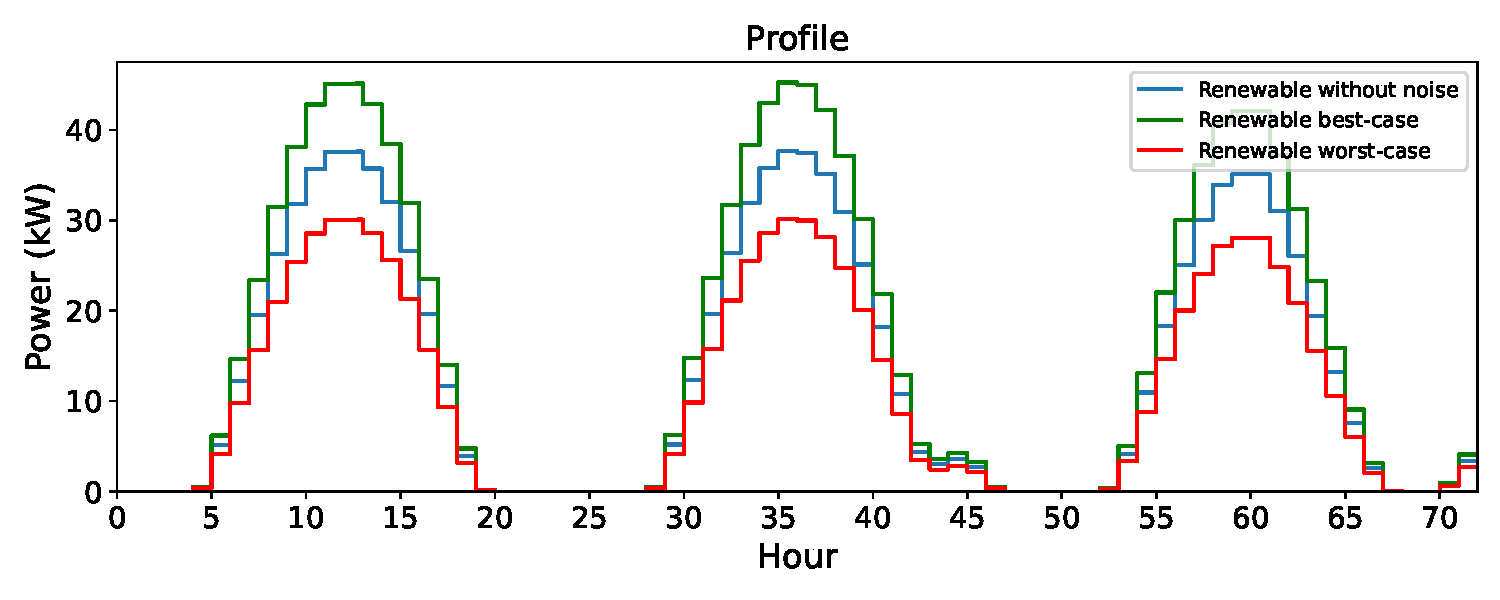
\includegraphics[scale=0.58]{Images/Compensations/critical_power_production_with_noise.pdf}
    \caption{The power production with noise for the critical scenarios.}
    \label{fig:critical_weather_with_noise}
\end{figure}

Regarding the workload, we introduced Gaussian noises in interarrival and job duration with a standard deviation of 20\% of the predicted value. The relation between these workload noises and the power demand is more complicated than the power production since the power demand depends on the scheduling algorithm and queue sort. Figure \ref{fig:critical_workload_with_noise} shows the impact of these noises on the power demand. Even if the impact on the workload power demand is not huge, these variances impact the offline IT plan since it will indicate the wrong moment to turn on/off the servers. The criticality of the workload comes from the moment where the jobs arrive (in the end or beginning).

\begin{figure}[!htb]
    \centering
    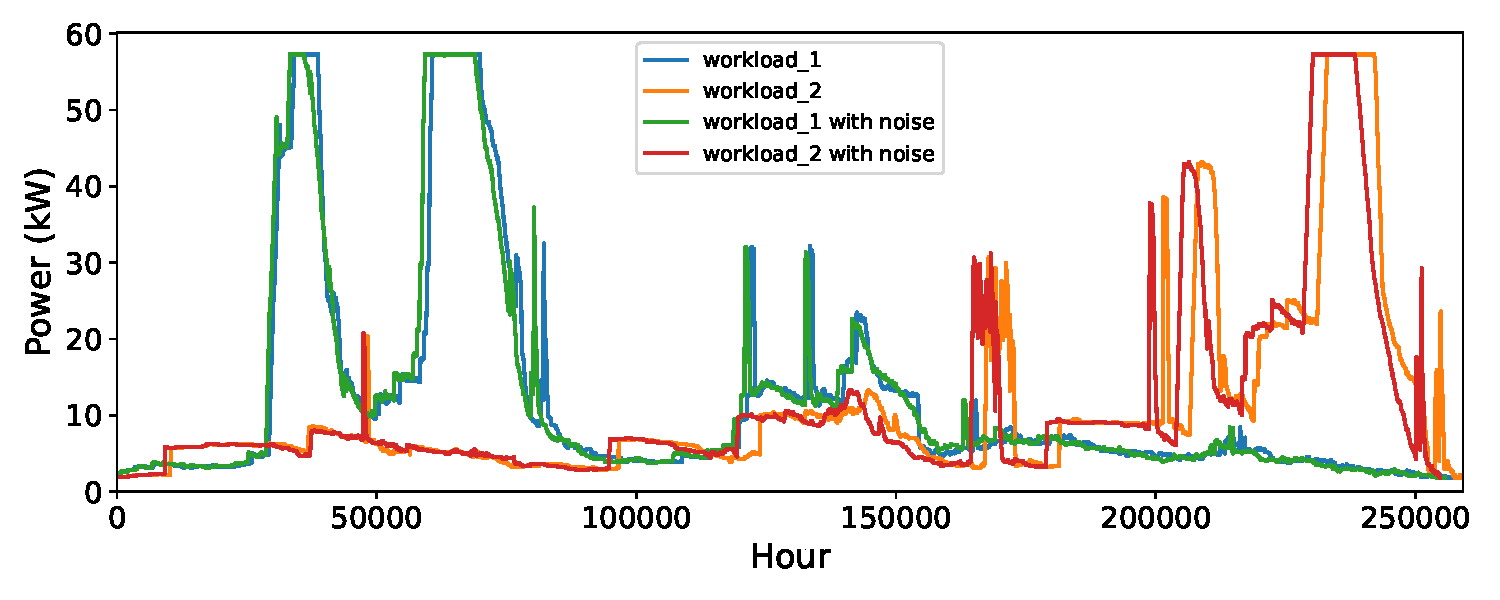
\includegraphics[scale=0.58]{Images/Compensations/critical_jobs_arriving_with_noise.pdf}
    \caption{The power demand with noise for the critical scenarios.}
    \label{fig:critical_workload_with_noise}
\end{figure}

Finally, we mixed the two productions (worst and best-case) with the two workloads (in the end and beginning), creating four scenarios:

\begin{enumerate}
    \item \emph{Critical 1}: Profile best-case and workload in the beginning;
    \item \emph{Critical 2}: Profile best-case and workload in the end;
    \item \emph{Critical 3}: Profile worst-case and workload in the beginning;
    \item \emph{Critical 4}: Profile worst-case and workload in the end;
\end{enumerate}

The first scenario is the best possible, with more energy and having all the jobs in the beginning. Therefore, the scheduler has the energy and time to decide when to place the jobs. However, the last scenario is the harder to make decisions, with lower energy and receiving the jobs at the very end.

\subsection{Average Scenarios}

In the \emph{Average Scenarios}, we chose 10 workload and weather traces. Figures \ref{fig:average_weather_with_noise} and \ref{fig:average_workload_with_noise} show the power production and demand, respectively. Then, we created 10 offline plans, one for each tuple of workload and profile. For example, workload 1 receives the production of profile 1, workload 2 receives profile 2, etc. The offline plans are created in the same way as the critical cases.

\begin{figure}[!htb]
    \centering
    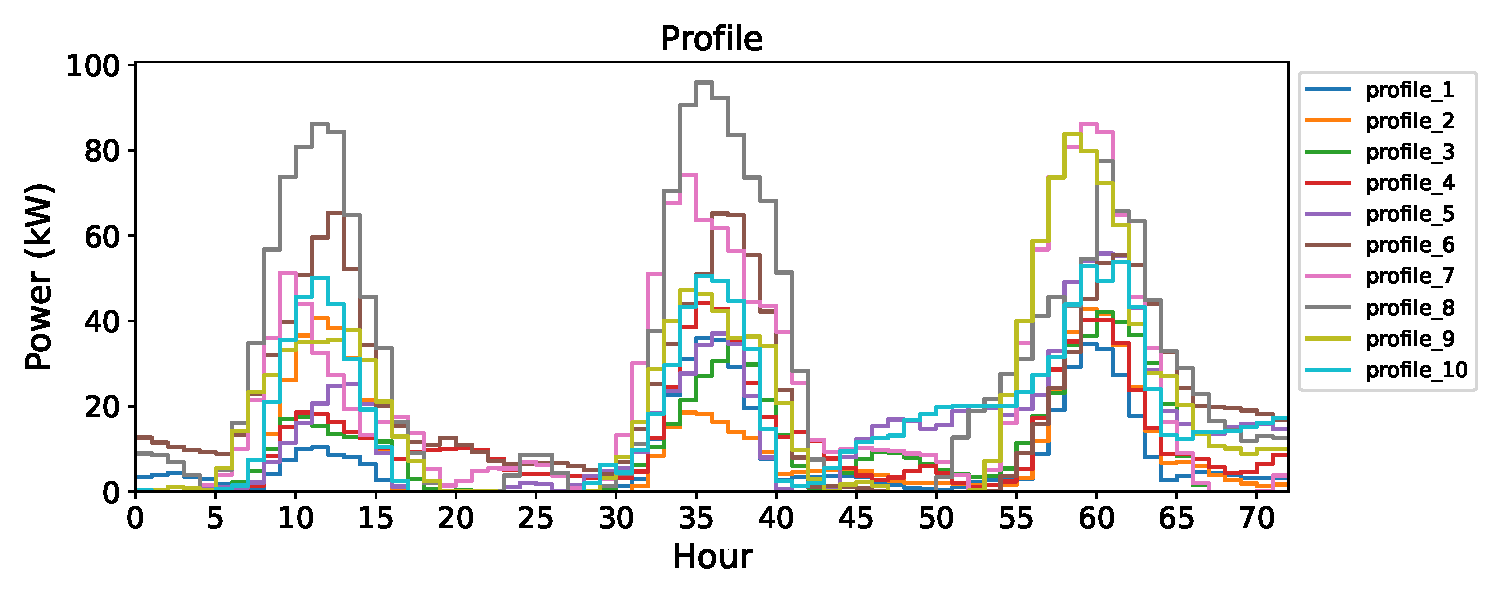
\includegraphics[scale=0.58]{Images/Compensations/diff_power_production.pdf}
    \caption{The power production for the average scenarios.}
    \label{fig:average_weather_with_noise}
\end{figure}

\begin{figure}[!htb]
    \centering
    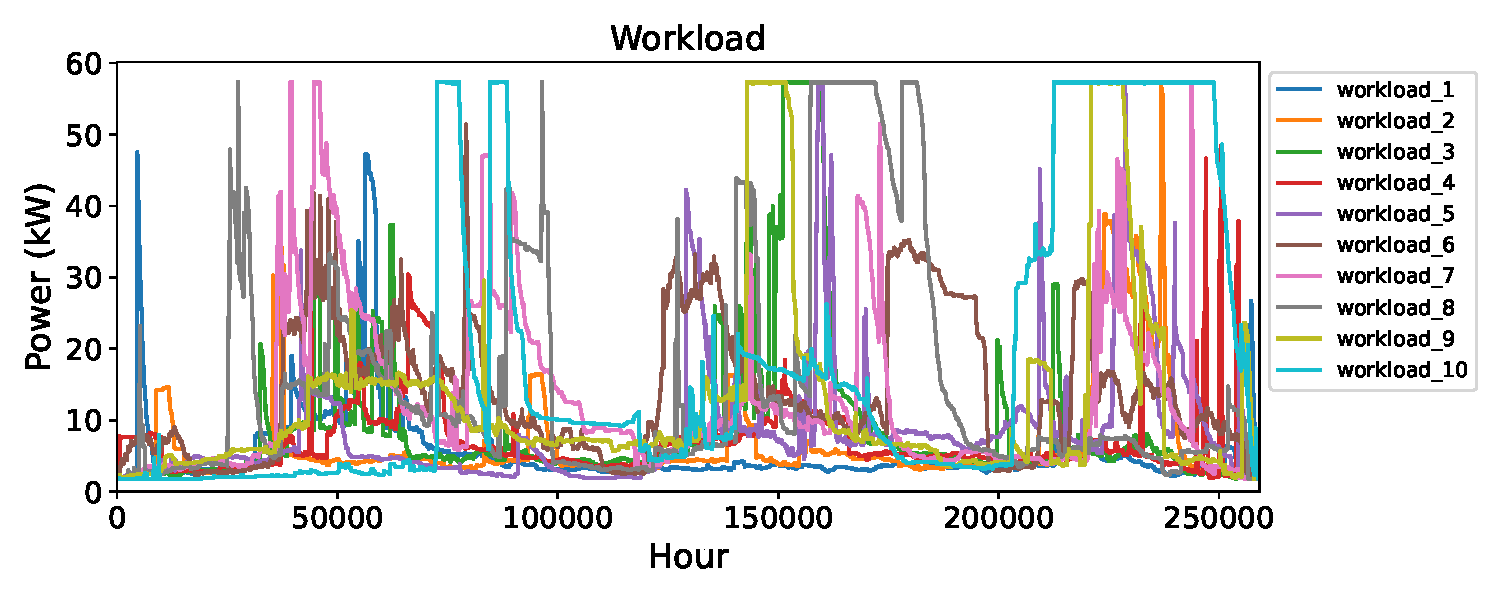
\includegraphics[scale=0.58]{Images/Compensations/diff_jobs_arriving.pdf}
    \caption{The power production for the average scenarios.}
    \label{fig:average_workload_with_noise}
\end{figure}

After creating the plans, we introduce noise in the values. Here, we applied Gaussian noises in power production, and jobs interarrival and size. We increase the standard deviation to 50\%, giving a larger range to generate values. Therefore, we have higher uncertainty. For each tuple (workload + profile), we generated 10 new workloads and profiles with noise, resulting in a total of 100 combinations. We called these scenarios as \emph{Average Scenarios} because they balance between positive and negative noises inside the same combination. In both parts (critical and average), besides the production and jobs noises, we have also the uncertainty from the walltime, presented in Section \ref{sec:workload_trace}.


\subsection{Baselines}
We created three baselines to compare the results from the four policies. The baselines are \emph{Follow plan}, \emph{Power reactive}, and \emph{Workload reactive}. \emph{Follow plan} is an algorithm that applies the offline plan without changing it. This algorithm emulates the execution of only the offline side. \emph{Power reactive} changes the server state according to the renewable power incoming. So, at each time step, it takes the power coming from renewable and calculates how many servers are possible to maintain running. It uses power from the batteries to maintain jobs running, if the renewable is not enough. \emph{Power reactive} uses the server configuration heuristic presented in Section \ref{sec:power_compensation}. \emph{Workload reactive} turns on the servers according to the job's arrival. It starts with all servers off. For each new job submitted, it turns on a server at maximum speed, if there is no server idle. After finishing a job, the server waits for $T_{wait}$ seconds (using the DPM technique from Equation \ref{equ:dpm_waiting_time}). If no job is placed on this server before $T_{wait}$, the scheduler sedates the server. In all cases (baselines and compensation policies), if the state of charge of the battery arrives at less than 20\% (defined $SoC_{min}$), the scheduler kills the jobs and sedates all servers. 

\section{Results Evaluation}

After describing the experimental environment, this section presents the results of the experiments. First, we discuss the critical cases. Then, we detail the results of the average cases.

\subsection{Critical cases}

\subsubsection{Scenario Critical 1}
Scenario Critical 1 (Profile best-case and workload in the beginning) is the case where the majority of jobs arrive at the beginning, and the production is higher than expected. However, this scenario is tricky. Since the battery starts with $SoC = 50\%$, if the scheduler starts too many jobs in the beginning, this can lead to a very low $SoC$ on the first day. This is exactly what happened with \emph{Workload reactive} in this scenario. Figure \ref{fig:DPM_soc} shows the evolution of the state of the charge in the \emph{Workload reactive} execution. At step 264 (79200 seconds after the simulation begins), \emph{Workload reactive} has less than 20\% of SoC. So, the scheduler kills the jobs. 

\begin{figure}[!htb]
    \centering
    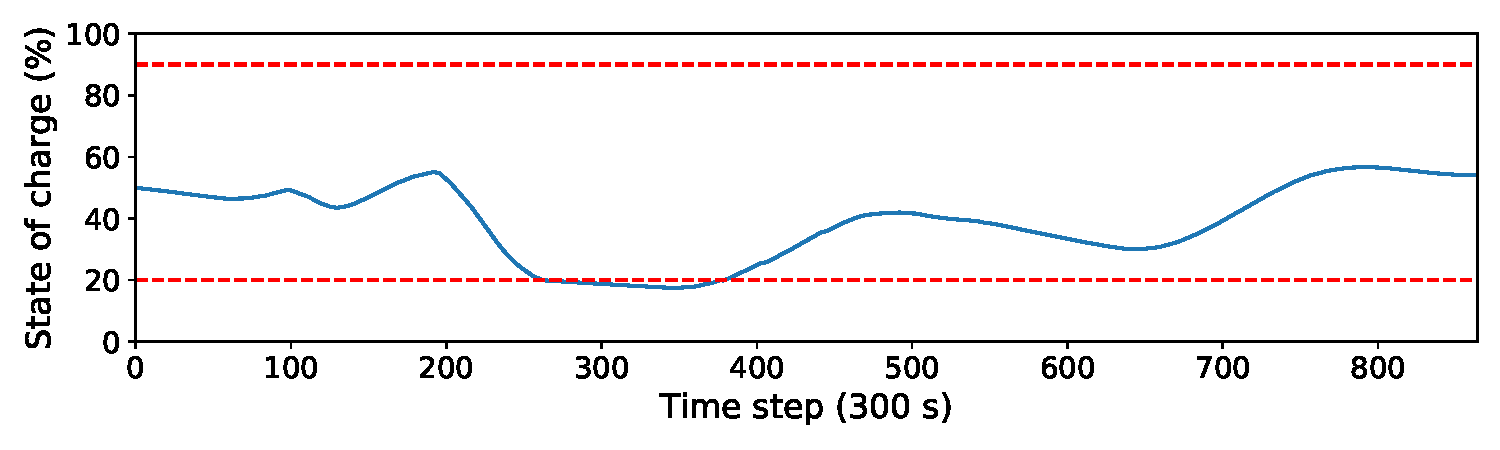
\includegraphics[scale=0.55]{Images/Compensations/critical_soc_s1.pdf}
    \caption{State of Charge for \emph{Workload reactive}.}
    \label{fig:DPM_soc}
\end{figure}

Figures \ref{fig:SoC_critical_1} and \ref{fig:jobs_critical_1} give the battery level at the end of the time window and jobs states, respectively. Figure \ref{fig:jobs_critical_1} shows two graphs. The first one considers only the number of jobs, ignoring their size. Therefore, all jobs are equal. In the second graph, we consider the size of the job. So, bigger jobs have more importance than smaller ones. The second graph illustrates the mass of work to do.

\begin{figure}[!htb]
    \centering
    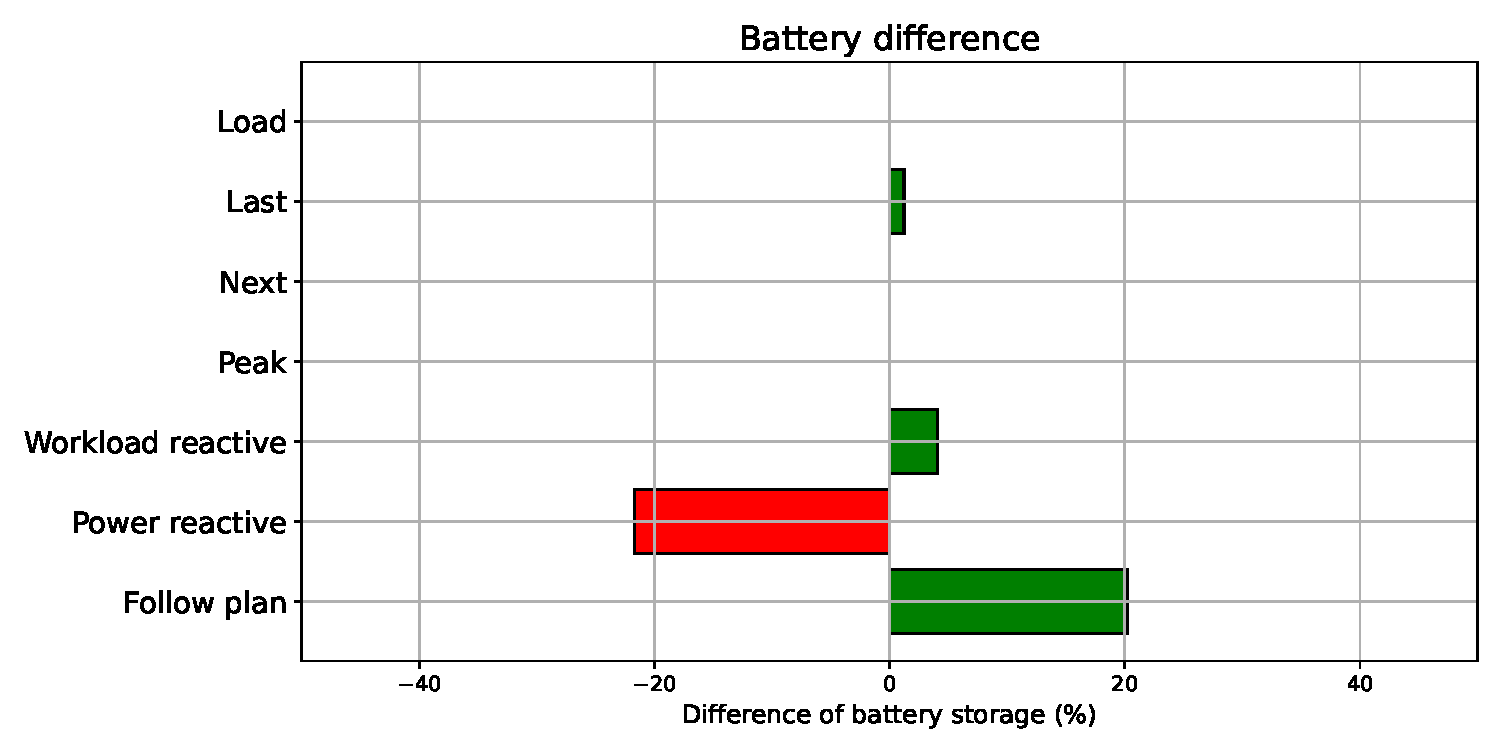
\includegraphics[scale=0.55]{Images/Compensations/battery_critical_1.pdf}
    \caption{Difference between the battery target level (50\%) and the real battery level at the end of the time window for scenario critical 1.}
    \label{fig:SoC_critical_1}
\end{figure}

\begin{figure}[!htb]
    \centering
    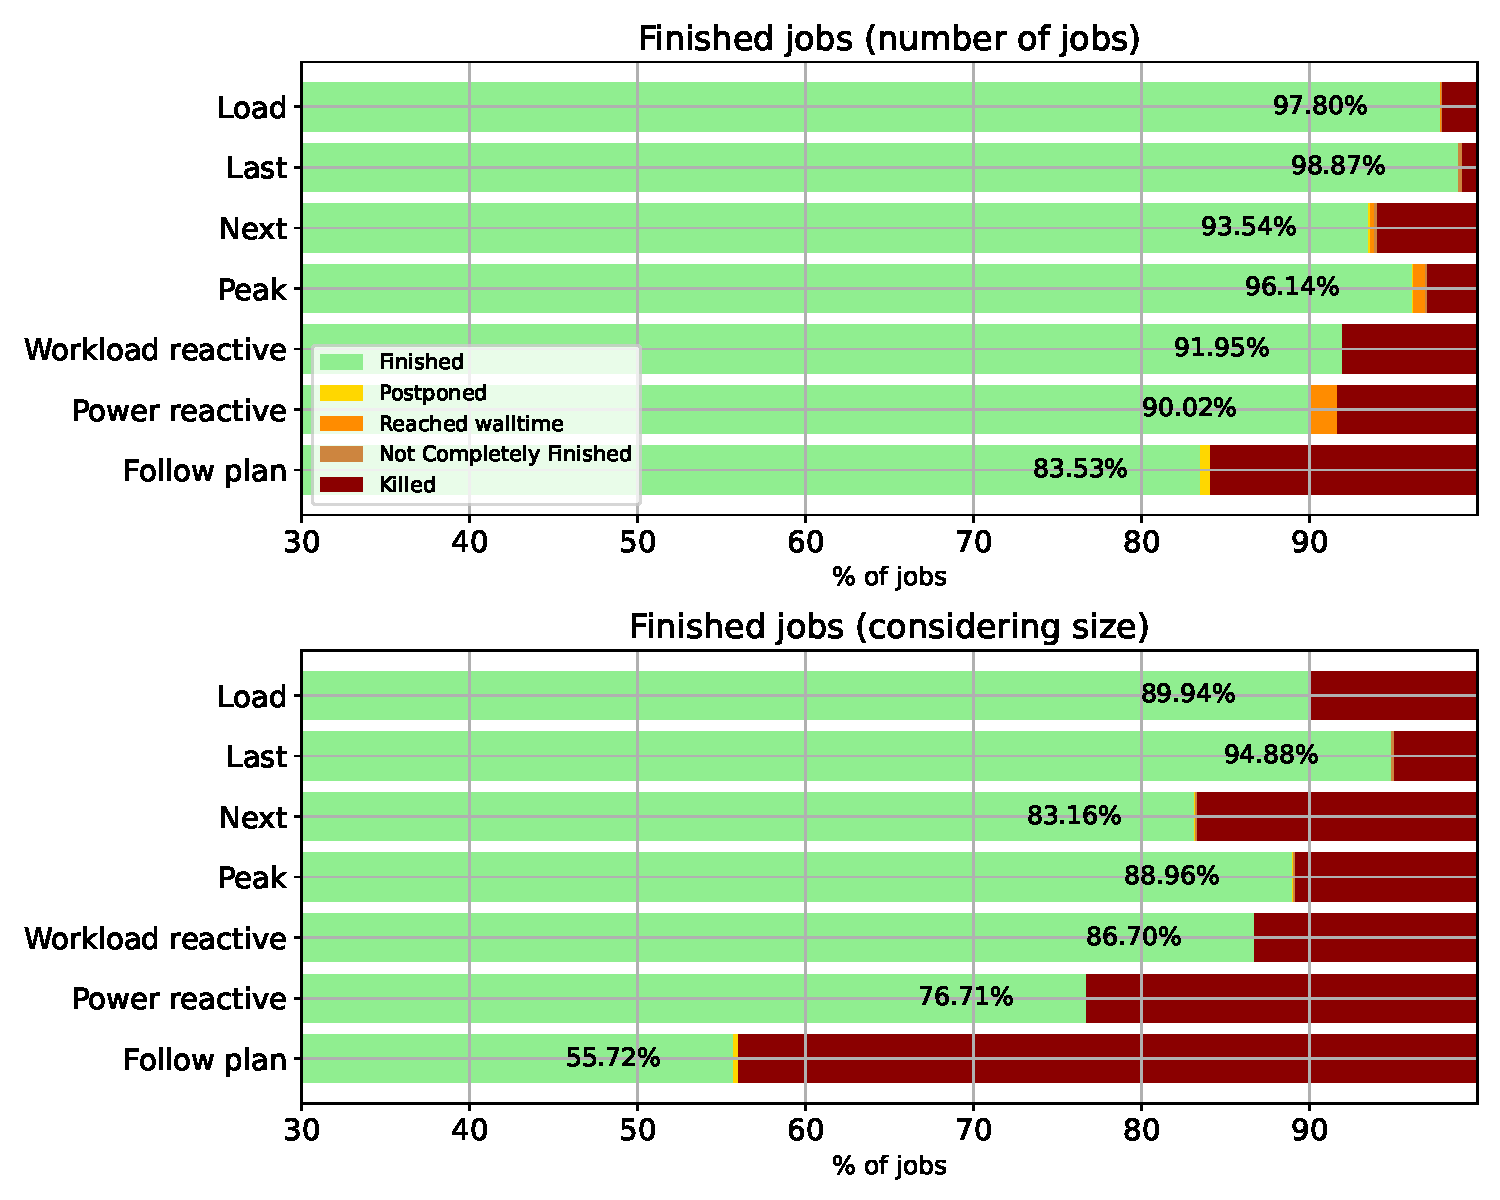
\includegraphics[scale=0.55]{Images/Compensations/jobs_critical_1.pdf}
    \caption{Jobs states at scenario critical 1. The first graph (above) considers only the number of jobs, ignoring their size. In the second graph (below), the jobs' size is considered.}
    \label{fig:jobs_critical_1}
\end{figure}

It is important to analyze the battery level and finished jobs together. For example, \emph{Follow plan} saves a lot of battery in this case, finishing with 20\% more energy than the target. This result seems very good, but analyzing the number of finished jobs, \emph{Follow plan} has the lower finished jobs and higher killed jobs. Also, it kills a lot of big jobs, resulting in only 55.72\% of finished jobs considering the size. This illustrates the importance of reacting to real events, using the saved energy to improve QoS. \emph{Follow plan} tends to kill bigger jobs since it does not adapt the plan to maintain them running.

\emph{Power reactive} has the worst battery level, with an SoC of around 28\% (difference of -21.729269\%). This algorithm allocates all incoming power from renewable sources to servers, not recharging the battery. The battery recharges a little bit due to power fluctuations (e.g., the server is idle so the incoming renewable power recharges the battery instead of going to the server). So, it uses the battery to avoid killing jobs, but it does not compensate for this change. \emph{Power reactive} is the second-worst finished jobs metric (ignoring or considering the size), with some jobs reaching the walltime. Since it only uses the battery to avoid killing jobs, sometimes it let the servers at slower speeds, increasing the possibility of reaching walltime. It also kills some jobs because it also reaches the $SoC_{min}$.

As mentioned at the beginning of this section, \emph{Workload reactive} can not manage well the state of charge, killing some jobs. Even so, it finishes with a good battery level. The DPM technique helps to save some energy, letting the incoming renewable to recharge the battery. Since it always put the servers at maximum speed, no job reached the walltime. It has the third-worst finished and killed jobs, considering the number of jobs. All the policies are very close to the target level. Just \emph{Last} policy saved a little bit more than the target, because it puts all the compensations in the end, and it can not use everything. Considering the metrics about the job, all policies finished more jobs and killed less than the three baselines. The best one is \emph{Last} with 98.87\% of the finished jobs considering the number of jobs and 94.88\% considering the size. Also, it has the lowest killed jobs. \emph{Load} places the compensations in the steps where it is expected to have higher demand. In this case, it pays off with the second-best results. We will see in future cases that this behavior is dangerous. 

\emph{Next} has the worst job result among the policies. It also kills more big jobs than the policies and \emph{Workload reactive}. This result can be explained by comparing \emph{Next} and \emph{Last}. For example, let's say we saved energy in step 0. So, \emph{Last} increase the usage in the last possible step. If at any moment between step 0 and the last step, it is necessary to use more energy, \emph{Last} can take the previous migration and use it now. On the other hand, \emph{Next} expended this energy as soon as possible. Therefore, \emph{Next} can arrive in some moments without energy to avoid killing jobs. Finally, \emph{Peak} has the third-best result, but with some jobs reaching the walltime. Since it shaves the power usage (negative/positive) peaks, it can reduce speed in critical moments (e.g., with a lot of jobs running). However, it can maintain the big jobs running. Even if \emph{Peak} finishes fewer jobs than \emph{Load} (difference of 1.66\%), \emph{Peak} approximates the finished jobs considering the size (difference of 0.98\%).

The second analysis is regarding wasted energy. Figure \ref{fig:energy_critical_1} shows the results. \emph{Workload reactive} turns on resources on demand and does not let idle servers available too much. Therefore, it has the best wasted energy metric compared with the other algorithms. The worst case is \emph{Power reactive} which turns on servers according to the power available and not the demand. \emph{Follow plan} and the four policies are guided by the offline plan. Therefore, the noise introduced in the real workload can lead to some mismatch between demand and production. Since \emph{Follow plan} kills more jobs than the policies, this metric is higher for this algorithm. The energy expended in killed jobs is considered wasted energy since the result of the killed job is useless. \emph{Last} has the second-best wasted energy since it runs more jobs than the other algorithms.

\begin{figure}[!htb]
    \centering
    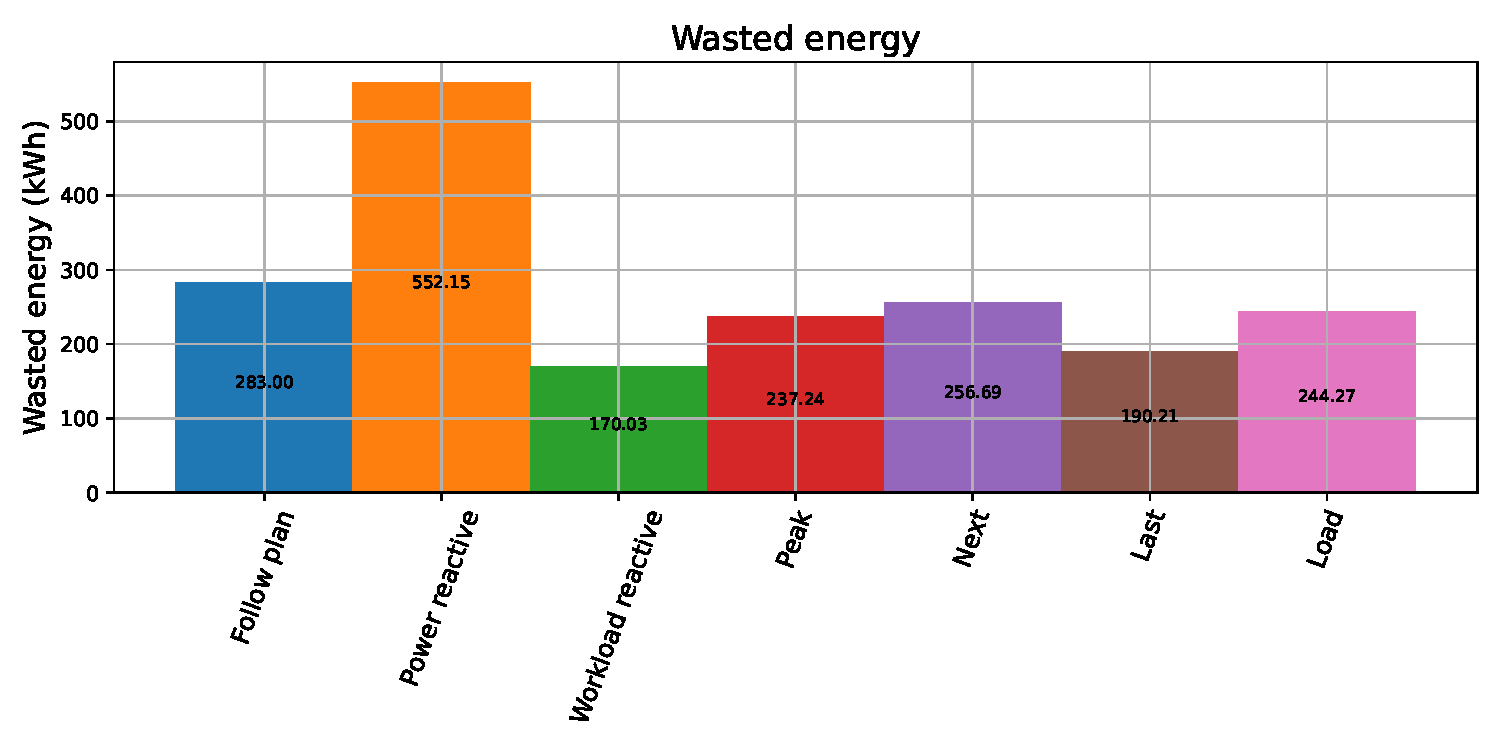
\includegraphics[scale=0.55]{Images/Compensations/energy_critical_1.pdf}
    \caption{Wasted energy at scenario critical 1.}
    \label{fig:energy_critical_1}
\end{figure}

Finally, Figure \ref{fig:slowdown_critical_1} demonstrates the slowdown of the finished jobs. As mentioned before, this metric is complicated to compare in an experiment with different numbers of finished jobs. We can see that \emph{Workload reactive} has some jobs with very high slowdown. It happens because stays a long period with the SoC below $SoC_{min}$ (as illustrated in Figure \ref{fig:DPM_soc}). So, it has a long period without servers running. \emph{Load} has a good mean and median. In this case, \emph{Load} can place the compensations close to the jobs' arrival. 

\begin{figure}[!htb]
    \centering
    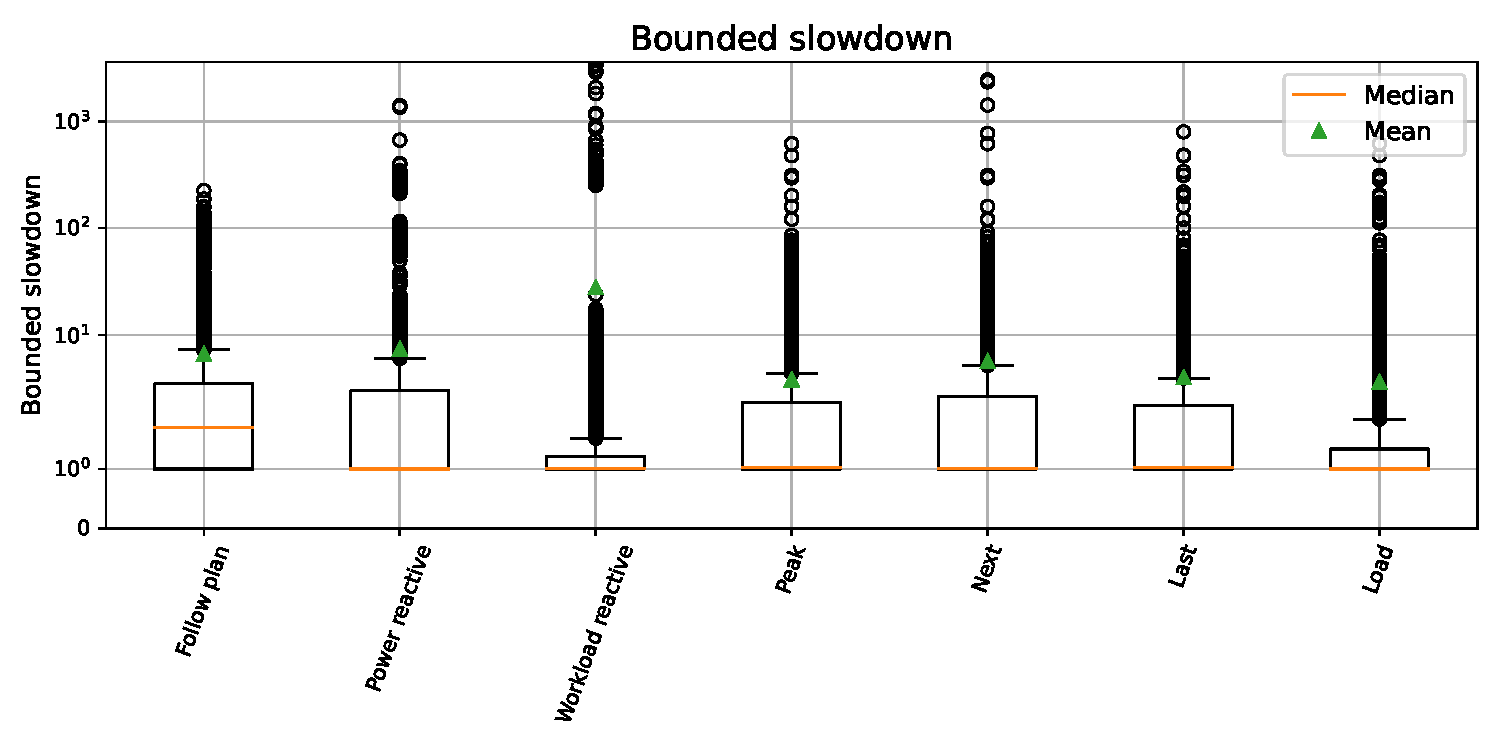
\includegraphics[scale=0.55]{Images/Compensations/slowdown_critical_1.pdf}
    \caption{Bounded slowdown at scenario critical 1.}
    \label{fig:slowdown_critical_1}
\end{figure}

\clearpage

\subsubsection{Scenario Critical 2}

Scenario Critical 2 has more energy than predicted (Profile best-case) and the jobs arriving in the end. In this scenario, the policies do not have much time to compensate, since the load comes on the last day. Figures \ref{fig:SoC_critical_2} and \ref{fig:jobs_critical_2} demonstrate the battery level and finished jobs. 

\begin{figure}[!htb]
    \centering
    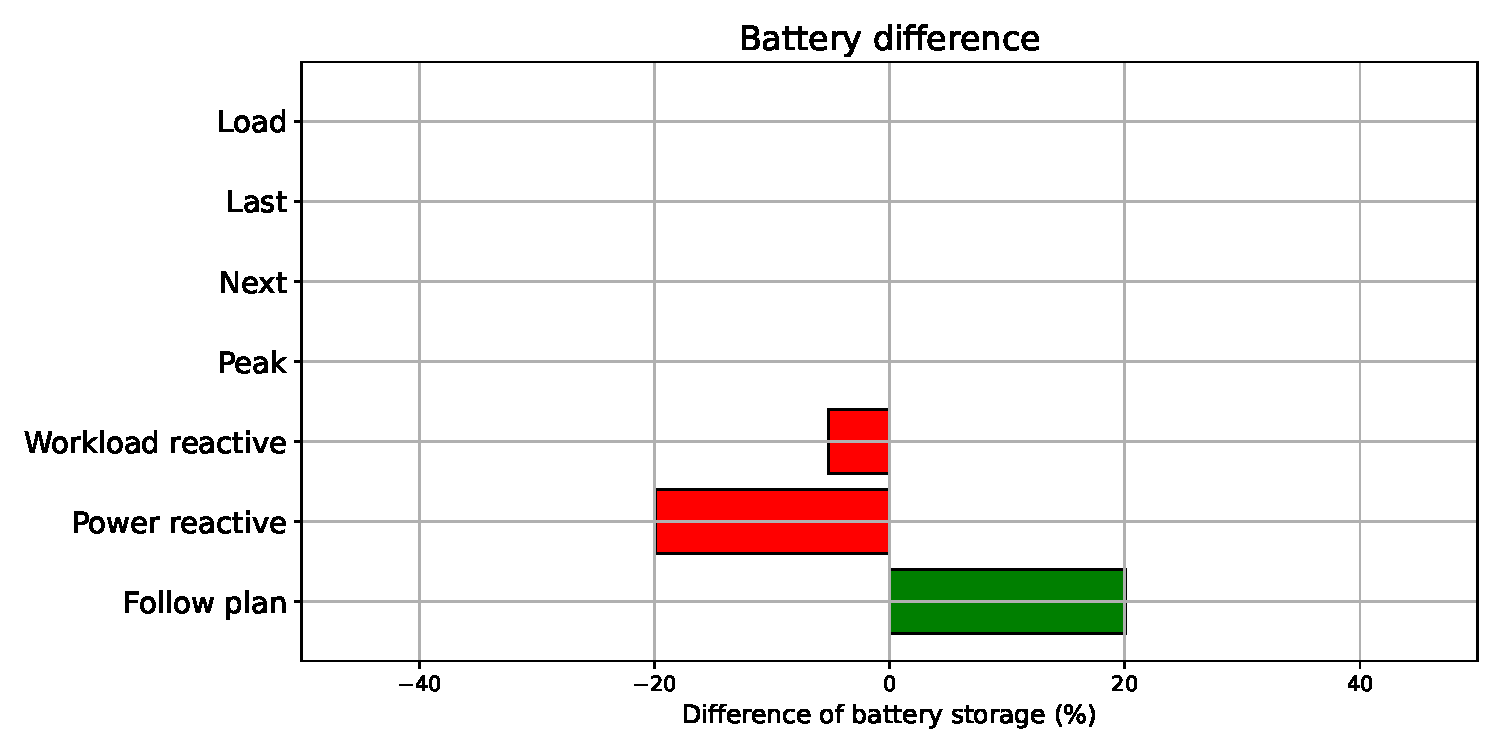
\includegraphics[scale=0.55]{Images/Compensations/battery_critical_2.pdf}
    \caption{Difference between the battery target level (50\%) and the real battery level at the end of the time window for scenario critical 2.}
    \label{fig:SoC_critical_2}
\end{figure}

\begin{figure}[!htb]
    \centering
    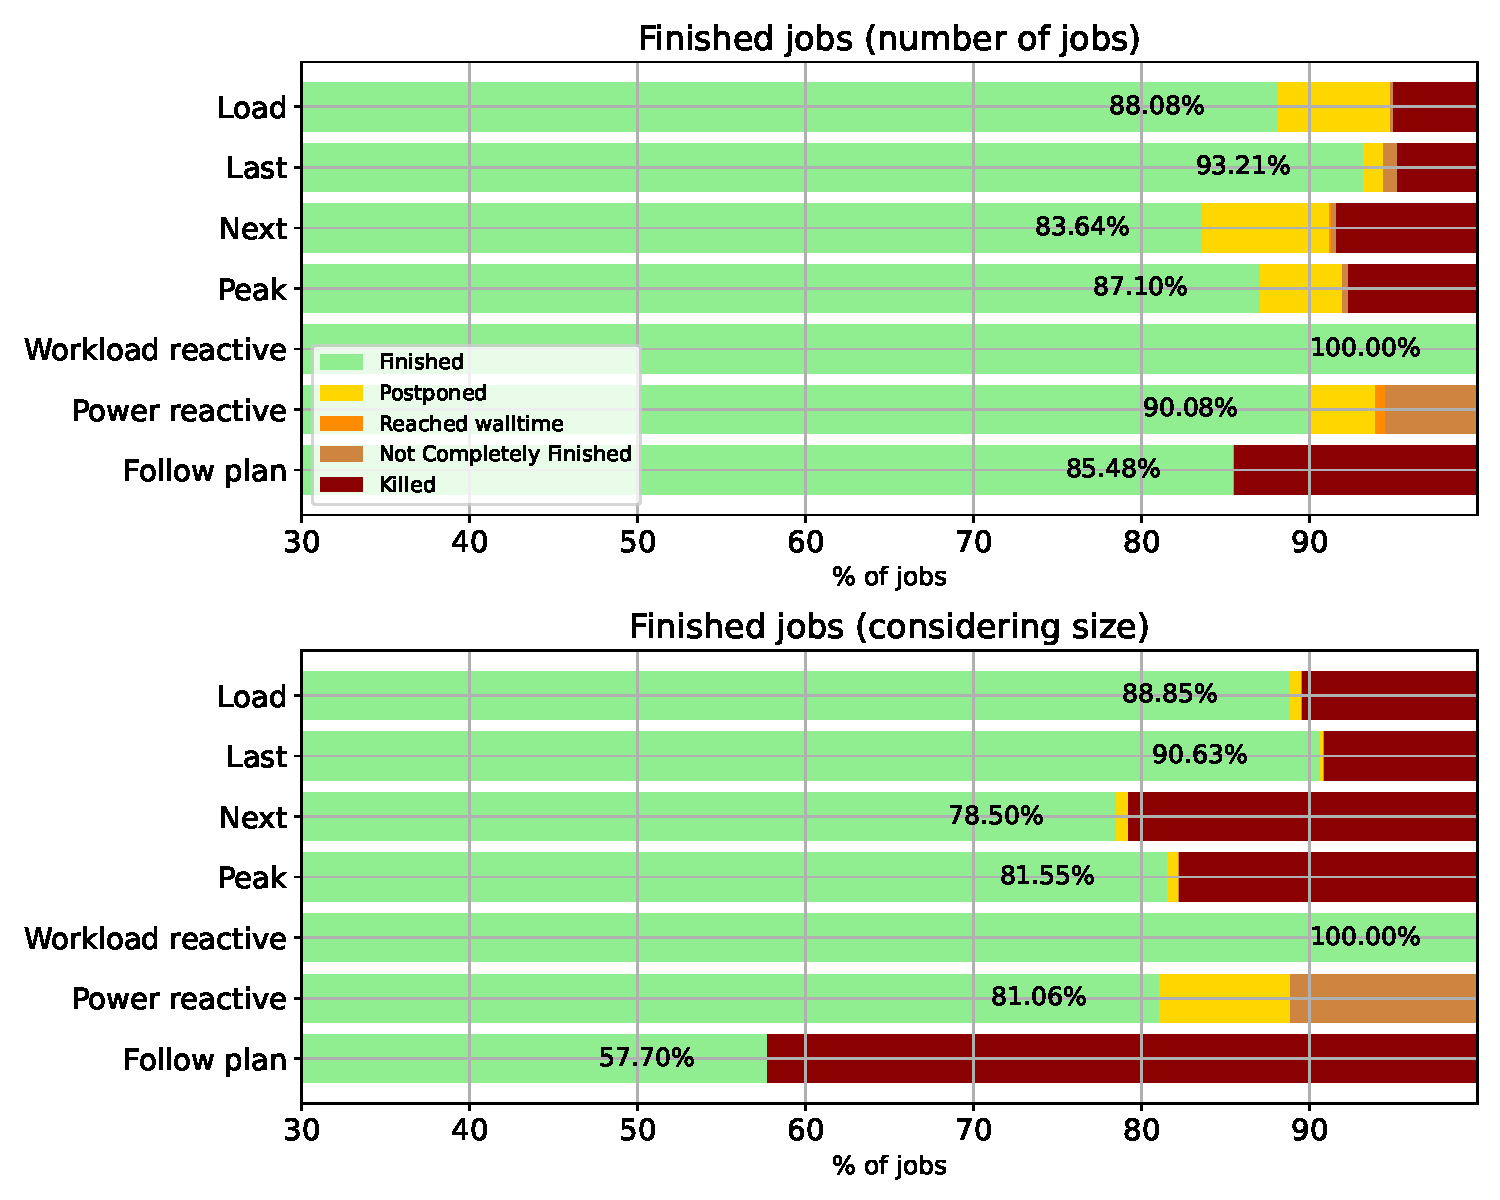
\includegraphics[scale=0.55]{Images/Compensations/jobs_critical_2.pdf}
    \caption{Jobs state at scenario Critical 2. The first graph (above) considers only the number of jobs, ignoring their size. In the second graph (below), the jobs' size is considered.}
    \label{fig:jobs_critical_2}
\end{figure}

\emph{Workload reactive} finished all jobs. This scenario is the best one for this algorithm since it can recharge the battery in the first two days, consuming all in the last day. Even so, it finishes with a battery deficit (-5.186277\%). \emph{Follow plan} has the second-worst finished jobs and the worst killed jobs considering the number of jobs, but finishing with a battery surplus of around 20\%. So, it misses the opportunity of using this surplus to avoid killing jobs. Considering the size, it kills more than 40\% of the jobs. \emph{Power reactive} has the third-best finished jobs considering the number of jobs, but with a good part not completely finished. These jobs are still running at the end of the time window, so we do not know if they would finish or not. However, it has the third-worst finished jobs considering the size of the jobs. Like in Scenario Critical 1, \emph{Power reactive} has a large battery deficit, with around -20\%. All policies have a perfect battery level, finishing with the SoC at around 50\% (the target level). All policies kill fewer jobs than the \emph{Follow plan}, using the higher-than-expected production to do so. However, they kill jobs to arrive at the battery target level, avoiding using more battery than predicted.

Just \emph{Next} policy finishes fewer jobs than \emph{Follow plan} considering the number, but more considering the size. This policy consumes all incoming energy as soon as possible, not having too much to use on the last day. \emph{Peak} has the third-worst finished jobs metric considering the number of jobs, worst than \emph{Power reactive}. This policy puts the surplus energy in the moment with less energy (negative peak). This behavior creates a more constant number of servers available during the time window. However, this case has a peak in the end, which makes this policy wastes resources. On the other hand, \emph{Peak} finishes more jobs than \emph{Power reactive} considering the size. It can finish bigger jobs due to its constant number of servers behavior. However, since the majority of jobs arrive at the end, it is better to place the positive compensations at the end (like \emph{Load} and \emph{Last}).

We can see a small difference in jobs finished (number of jobs) between \emph{Peak} and \emph{Load}, where \emph{Load} puts the energy in the moments with a higher difference between demand and production. It helps to increase almost 1\% of finished jobs and decreases around 2\% of killed jobs. Also, \emph{Load} can increase the number of bigger jobs finished compared to the \emph{Peak} policy. Nevertheless, the best results come from \emph{Last}. This policy stock all surplus at the last moment, allowing to execute more jobs. It can finish 3.13\% (number of jobs) more than the third-best, the only above 90\% finished jobs considering the size (besides \emph{Workload reactive}), and having a perfect level of battery at the end of the time window.

Considering the wasted energy, Figure \ref{fig:energy_critical_2} illustrates the results in this scenario. Again, \emph{Workload reactive} has the best result due to its workload reactiveness approach. The worst one is \emph{Power reactive}, for the same reason as scenario Critical 1. It turns on and increases the speed according to the power incoming, and not the demand. \emph{Follow plan} has not-so-bad wasted energy, even with a high number of killed jobs. \emph{Peak} and \emph{Next} wasted more than the \emph{Follow plan}. Both policies place the energy at the wrong moments. For example, if \emph{Next} has a positive compensation (increase the usage) in step 1, it will increase the usage in step 2. However, the demand is in the end. Then, the energy is wasted on idle servers. \emph{Peak} policy will do something similar, but putting in the negative peak. With the load in the beginning, it was not a problem for \emph{Peak} (it can delay the jobs for executing later). Nevertheless, in this scenario, it lets the servers idle. On the other hand, \emph{Last} and \emph{Load} have better energy usage than the \emph{Follow plan}. Both policies put the energy in the right moment (last steps).

\begin{figure}[!htb]
    \centering
    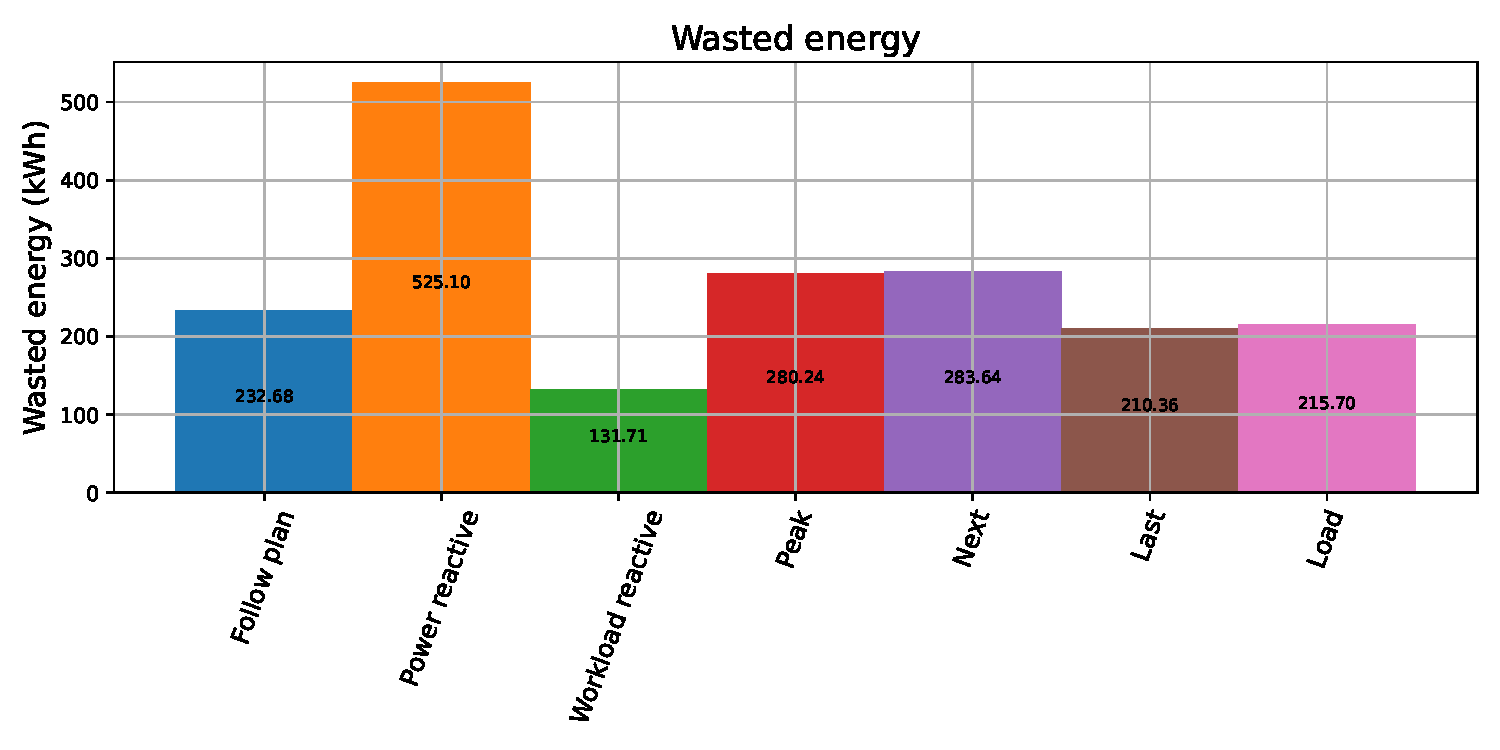
\includegraphics[scale=0.55]{Images/Compensations/energy_critical_2.pdf}
    \caption{Wasted energy at scenario Critical 2.}
    \label{fig:energy_critical_2}
\end{figure}

Regarding the bounded slowdown, Figure \ref{fig:slowdown_critical_2} shows the results. \emph{Workload reactive} has the best results due to its workload reactiveness. Without the SoC problem from the previous scenario, it can execute all jobs as soon as they arrive. The policies present a better median than \emph{Follow plan} but a higher mean, due to several jobs with bounded slowdown higher than 100. Yet, since \emph{Last}, \emph{Peak}, and \emph{Load} finish more jobs than \emph{Follow plan}, it is complicated to compare them.

\begin{figure}[!htb]
    \centering
    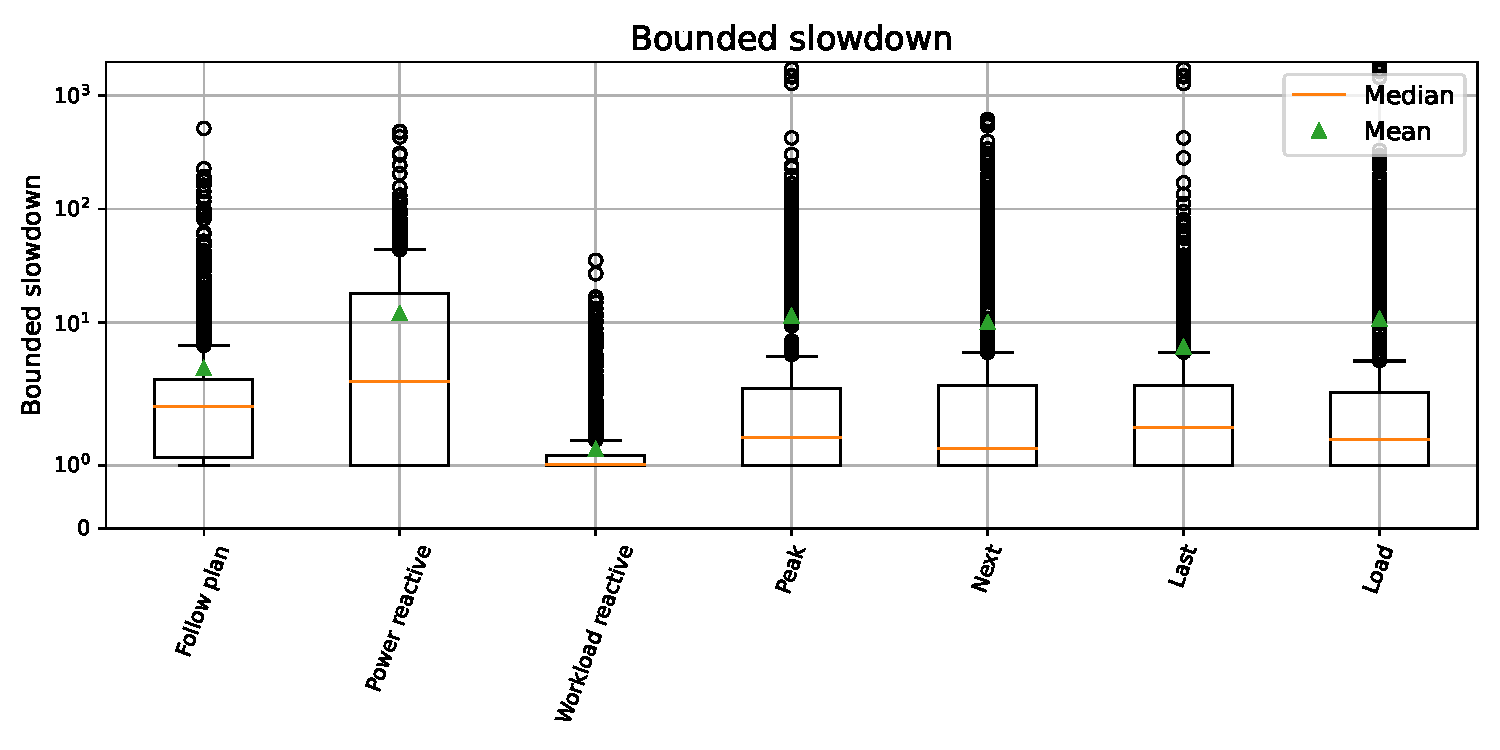
\includegraphics[scale=0.55]{Images/Compensations/slowdown_critical_2.pdf}
    \caption{Bounded slowdown at scenario Critical 2.}
    \label{fig:slowdown_critical_2}
\end{figure}

\clearpage

\subsubsection{Scenario Critical 3}
Scenario 3 introduces less energy than predicted with the jobs arriving on the first day. Figure \ref{fig:SoC_critical_3} gives the final battery level in this scenario. This figure demonstrates that the policies finished closer to the target level than the baselines, with -6.177244\% in the worst case (\emph{Load}). This scenario is particularly difficult to finish at 50\% since the policies migrate power to the first day expecting to compensate for it on the second and third days. However, it receives less energy than expected, being a little far from the target level. Nevertheless, the policies are way better compared to the \emph{Workload reactive}, \emph{Power reactive}, and \emph{Follow plan}.

\begin{figure}[!htb]
    \centering
    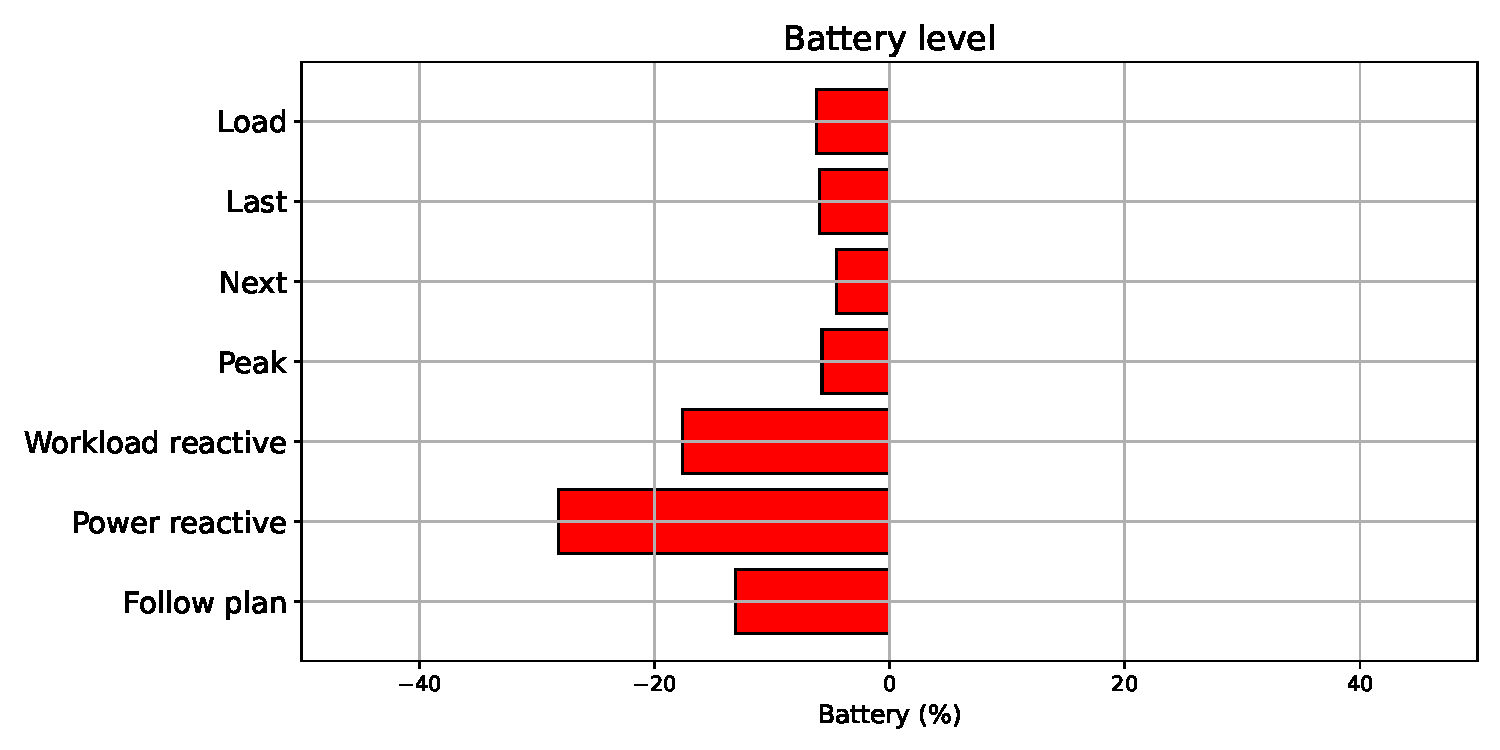
\includegraphics[scale=0.55]{Images/Compensations/battery_critical_3.pdf}
    \caption{Difference between the battery target level (50\%) and the real battery level at the end of the time window for scenario critical 3.}
    \label{fig:SoC_critical_3}
\end{figure}

Concerning finished jobs, Figure \ref{fig:jobs_critical_3} illustrates the results. As presented in scenario 1, \emph{Workload reactive} has a problem in the scenario with the peak of load in the beginning because it will place all jobs as soon as they arrive. We can see that scenario 3 is even worst, having more than 20\% killed jobs considering the number and more than 40\% considering the size of the jobs. \emph{Power reactive} finishes more jobs than any other algorithm, with 85.60\% (number of jobs) and 61.43\% (considering size). This algorithm follows the real production to set the servers' speeds. This behavior helps to start several jobs, but it can not maintain the jobs running when the battery arrives at $SoC_{min}$. So, it has more than 10\% of killed jobs considering the number and almost 40\% considering the size. \emph{Follow plan} finishes more jobs than the policies in both number and size. However, it kills several jobs, with almost 20\% in number and almost 50\% in size (the worst result). 

\begin{figure}[!htb]
    \centering
    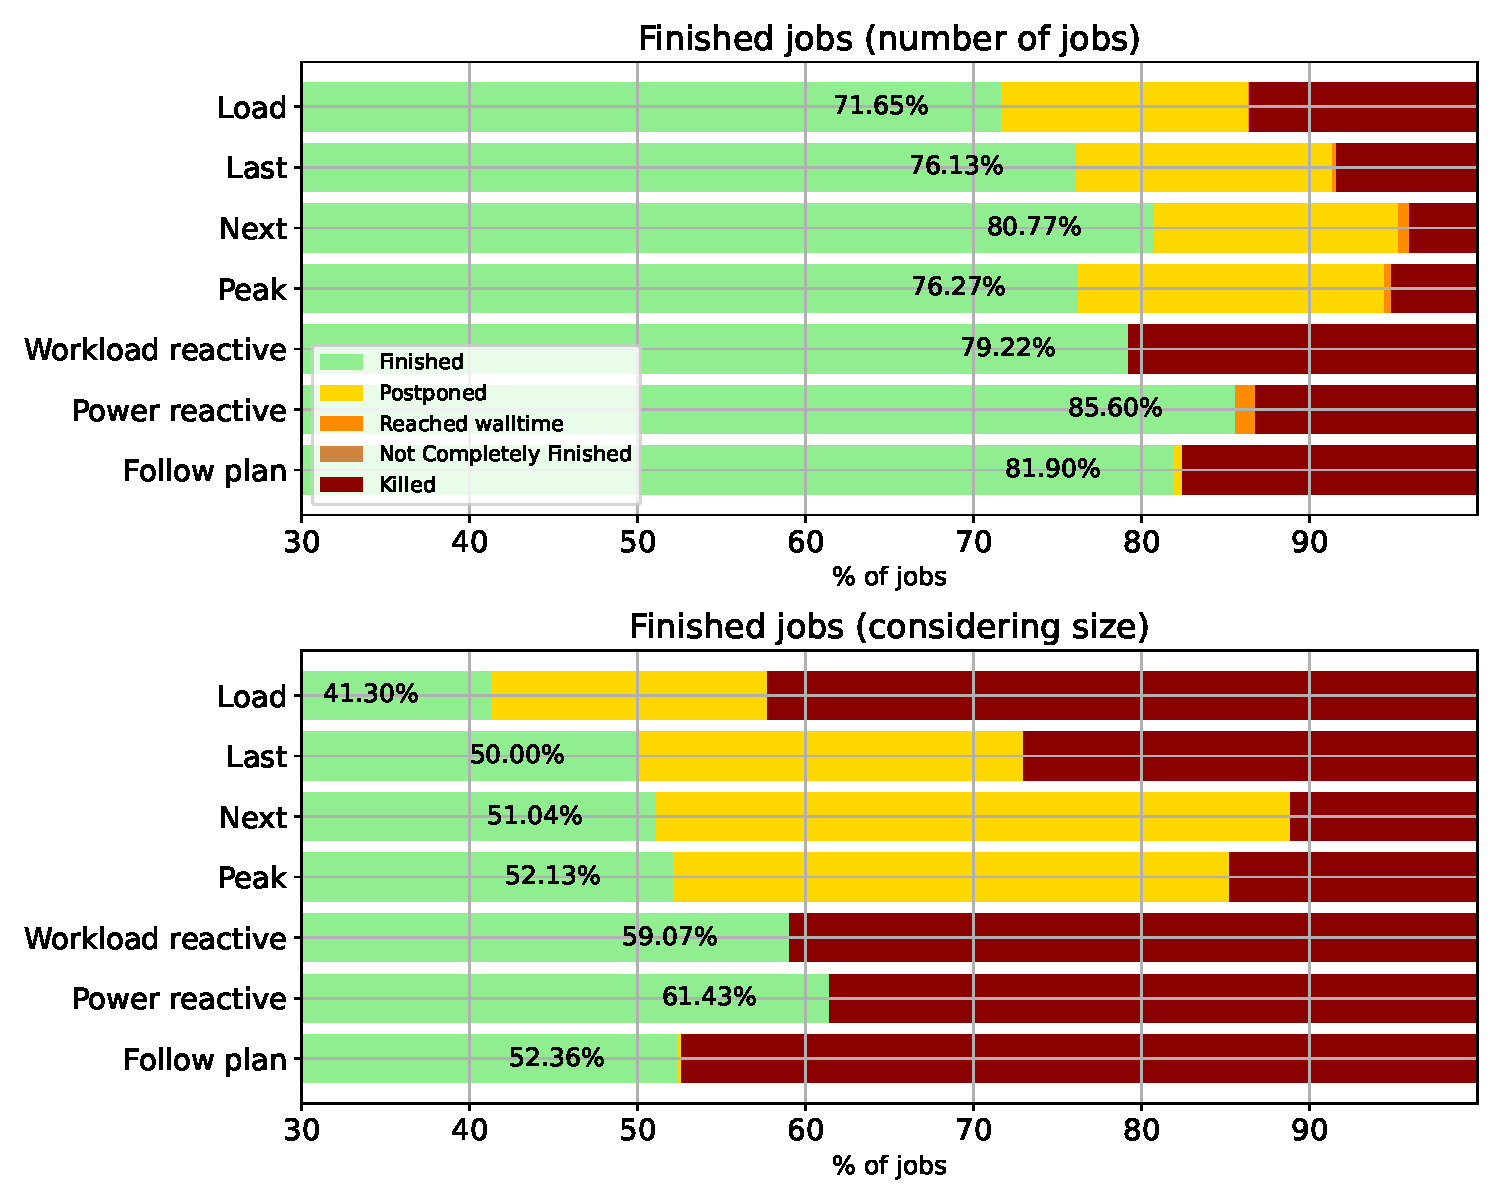
\includegraphics[scale=0.55]{Images/Compensations/jobs_critical_3.pdf}
    \caption{Jobs state at scenario critical 3. The first graph (above) considers only the number of jobs, ignoring their size. In the second graph (below), the jobs' size is considered.}
    \label{fig:jobs_critical_3}
\end{figure}

Among the policies, \emph{Load} has the worst result of finished and killed jobs in both number and size, compared to the other policies. In this scenario, \emph{Load} puts any positive compensation on the first day, approximating too fast to $SoC_{min}$. Then, it has to kill several jobs to avoid this boundary. This result shows that the \emph{Load} aggressivity does not pay off always. On the other hand, \emph{Next} stays close to the SoC planned. In this case, it can manage better the SoC, finishing more than 80\% jobs in number. Among the policies, \emph{Next} is only worst than \emph{Peak}. As mentioned before, \emph{Peak} can smooth the peaks maintaining more servers available constantly. We can see that it finishes fewer jobs in number than \emph{Next} but more in size. \emph{Peak} has a similar result than \emph{Follow plan}, using less battery and killing less jobs. Another result that confirms the need for reactivity.

Figure \ref{fig:energy_critical_3} shows the wasted energy in this scenario. We can see that all policies present lower wasted energy than the baselines, a very important result in a scenario with less energy available. \emph{Next} policy wasted 45.96\% less energy than \emph{Workload reactive} (the best baseline). \emph{Load} has the worst wasted energy among the policies, due number of killed jobs. The energy expended in killed jobs is considered wasted. Even so, \emph{Power reactive} has lower killed jobs than \emph{Load} but it has higher wasted energy. \emph{Power reactive} follows the power available, turning on servers according to the power available. Therefore, it expends more energy than the other algorithms in transition states.

\begin{figure}[!htb]
    \centering
    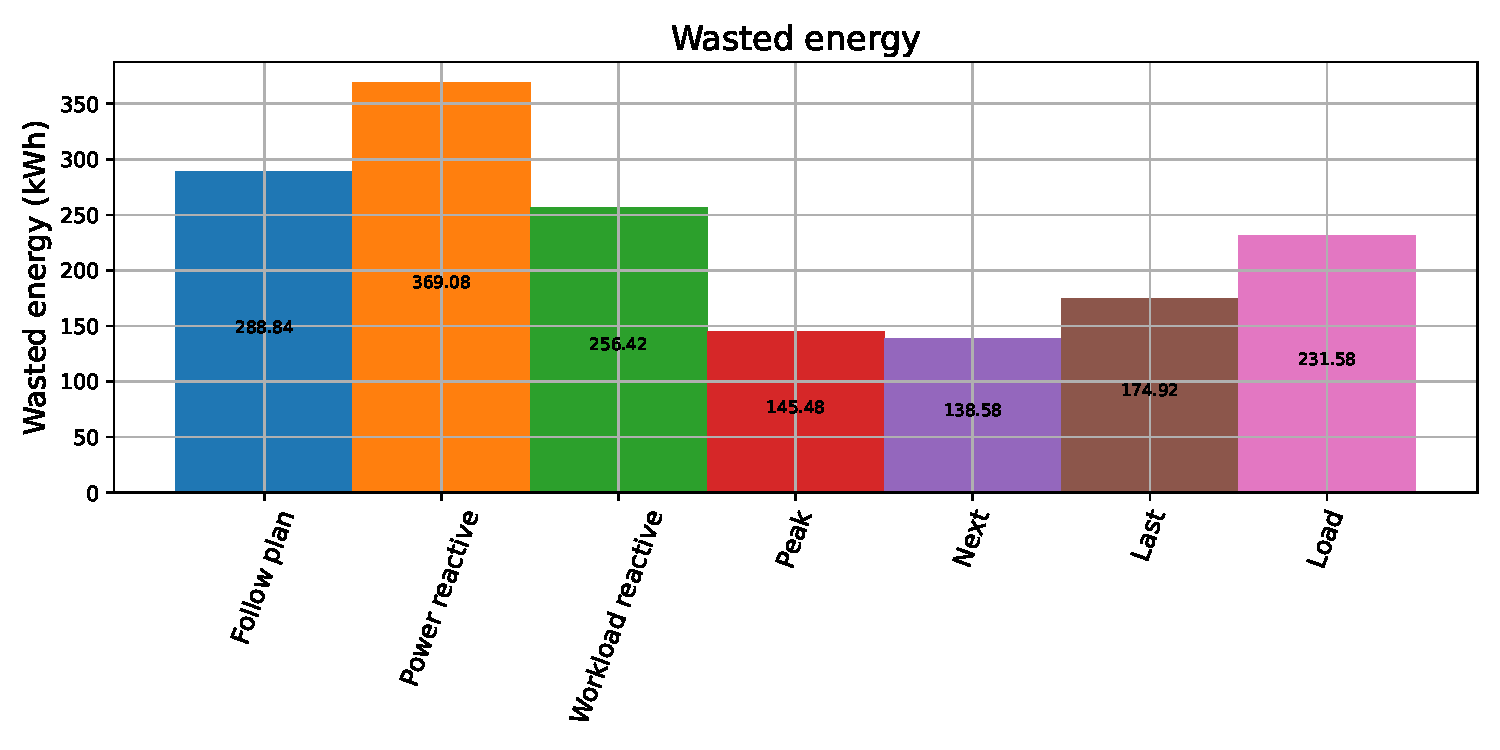
\includegraphics[scale=0.55]{Images/Compensations/energy_critical_3.pdf}
    \caption{Wasted energy at scenario critical 3.}
    \label{fig:energy_critical_3}
\end{figure}

Finally, Figure \ref{fig:slowdown_critical_3} shows the bounded slowdown. \emph{Workload reactive} has a similar result to Scenario 1. When it arrives at $SoC_{min}$, it has a long time without servers available, increasing the waiting time and slowdown for some jobs. However, it still has a very low median, showing that the majority of the jobs have a very small slowdown. In this scenario, the policies let the jobs wait longer, delaying the starting time for the moment with enough energy to finish them. So, the policies have higher mean and median slowdown. 

\begin{figure}[!htb]
    \centering
    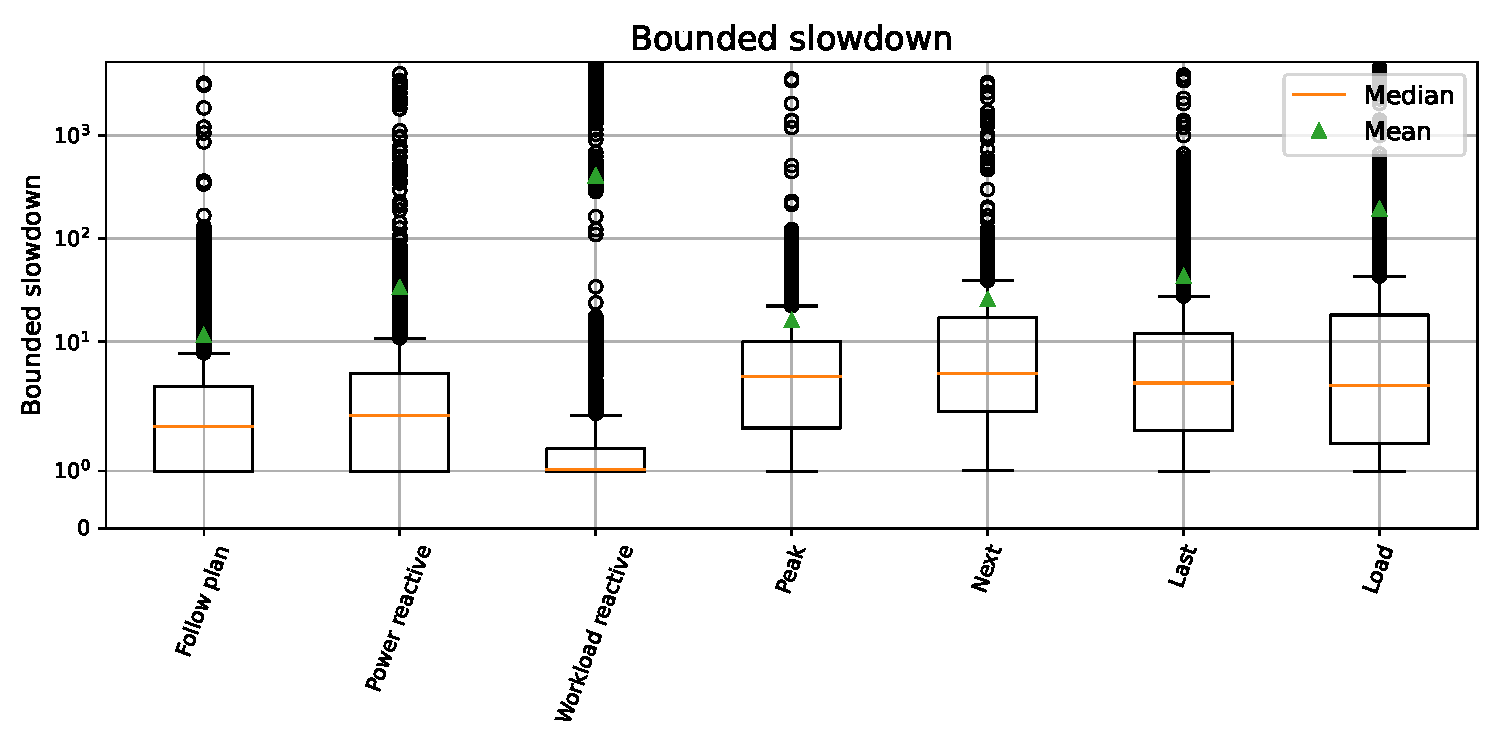
\includegraphics[scale=0.55]{Images/Compensations/slowdown_critical_3.pdf}
    \caption{Bounded slowdown at scenario critical 3.}
    \label{fig:slowdown_critical_3}
\end{figure}

\clearpage

\subsubsection{Scenario Critical 4}

The last critical scenario is the harder one, with less energy and jobs arriving in the end. Figure \ref{fig:SoC_critical_4} shows the impact on the battery level. Both \emph{Workload reactive} and \emph{Power reactive} finished with a deficit higher than 30\%, with 31.45\% and 30.78\%. Both ended the battery with less than the $SoC_{min}$ of 20\% (18.55\% and 19.22\%). \emph{Follow plan} finished with the SoC at 35.72\% (-14.28\%), being far from the target level. Nevertheless, the policies finished very close to 50\%. Since the first two days provide less energy, the policies can adapt the usage of the last day to approximate the target level. However, Figure \ref{fig:jobs_critical_4} shows the impact on QoS.

\begin{figure}[!htb]
    \centering
    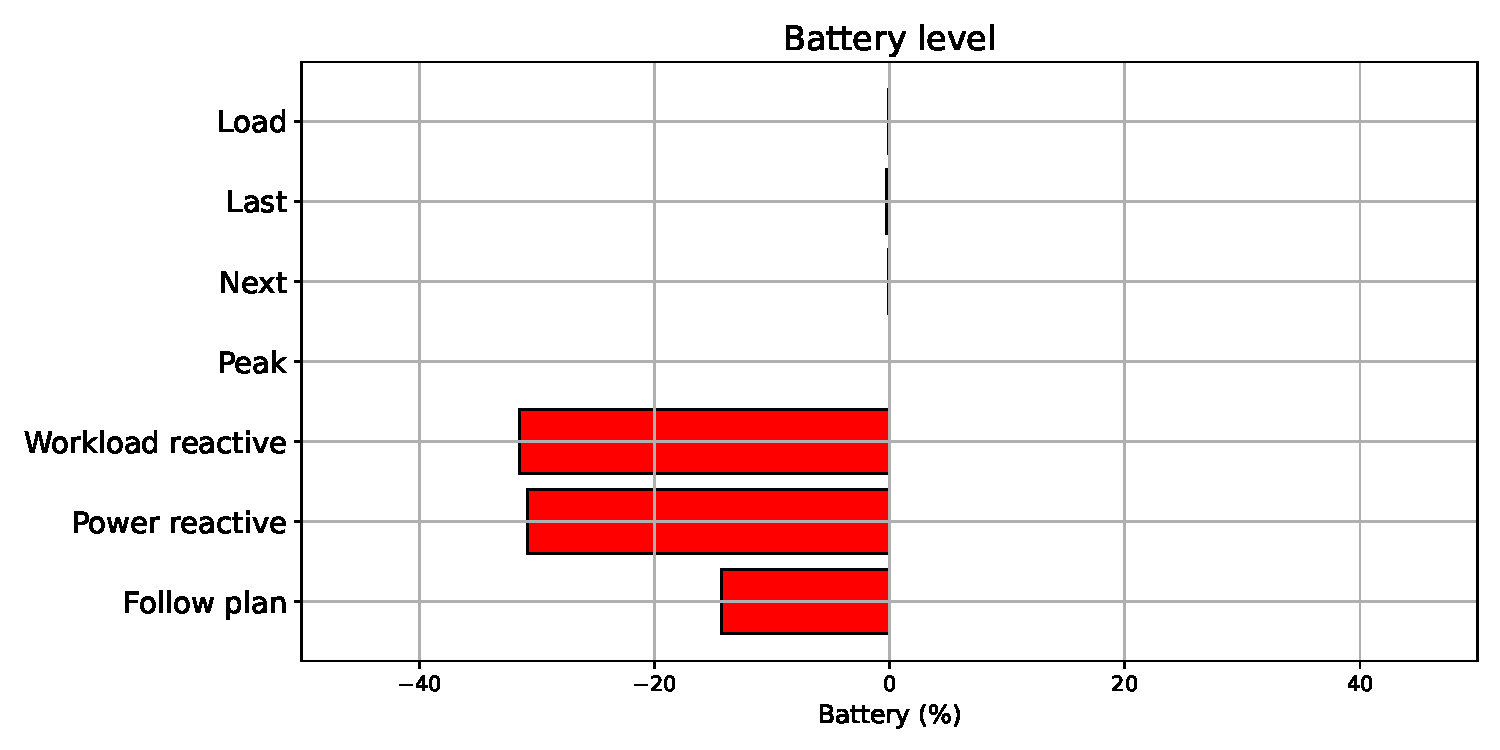
\includegraphics[scale=0.55]{Images/Compensations/battery_critical_4.pdf}
    \caption{Difference between the battery target level (50\%) and the real battery level at the end of the time window for scenario critical 4.}
    \label{fig:SoC_critical_4}
\end{figure}

\begin{figure}[!htb]
    \centering
    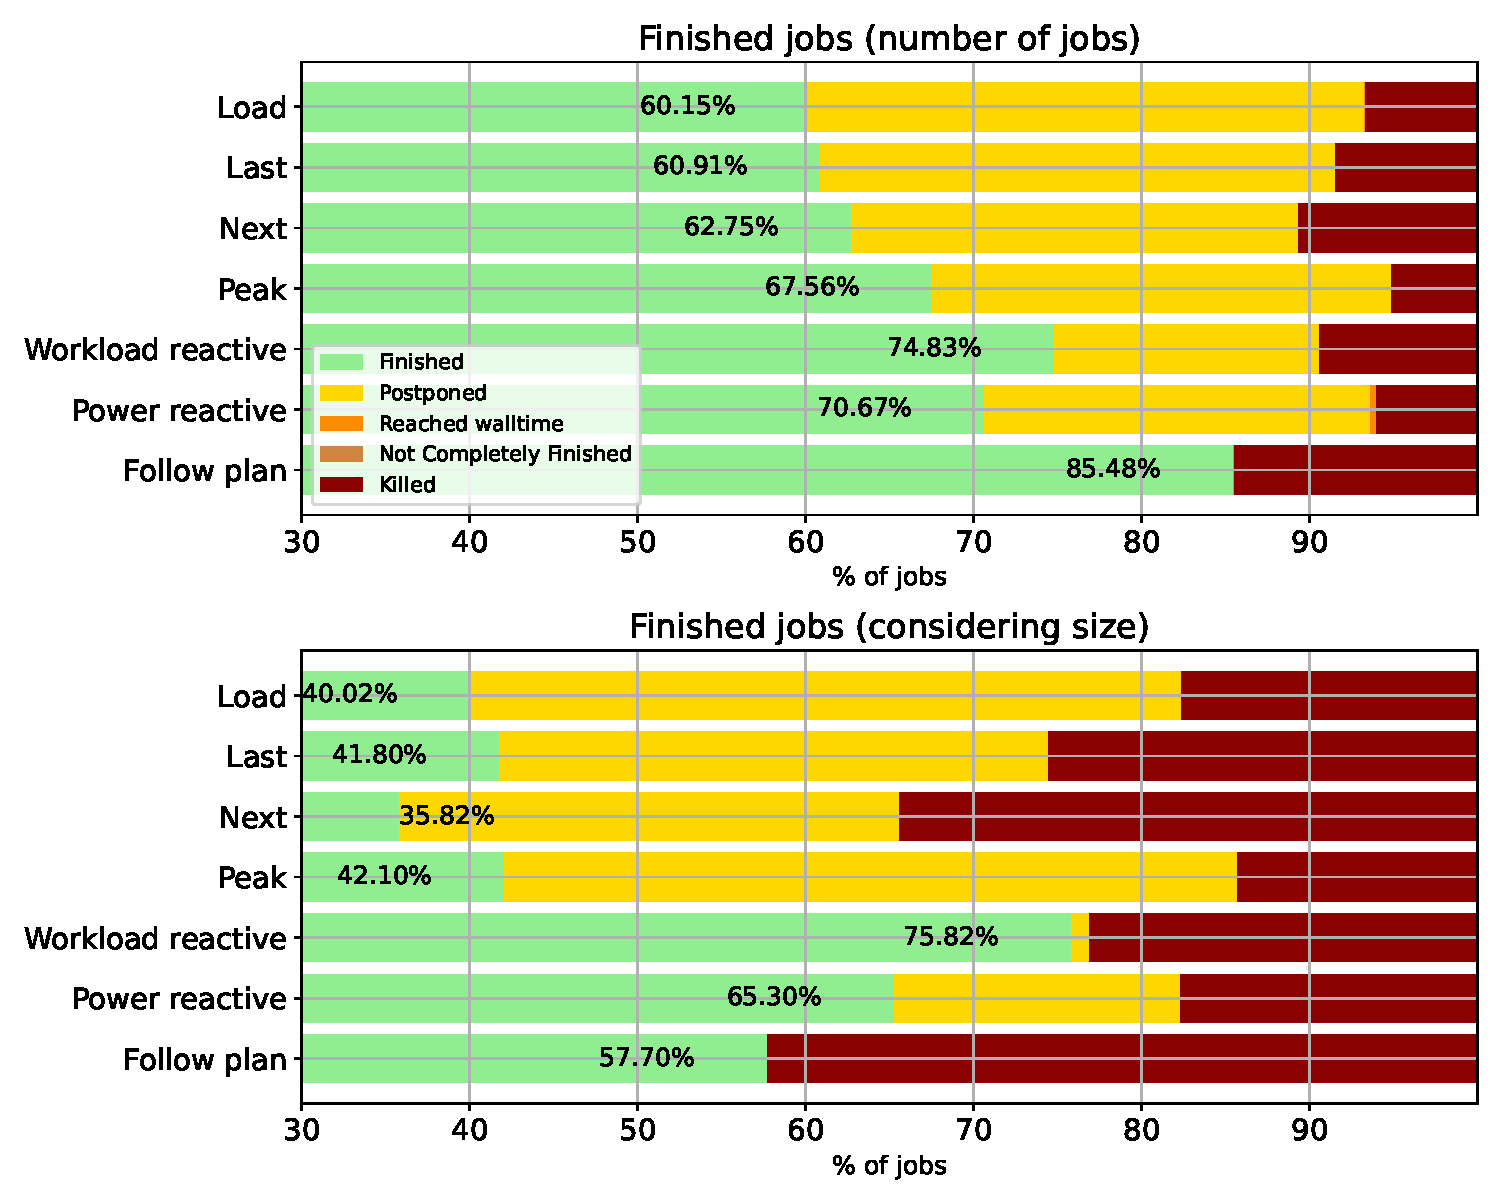
\includegraphics[scale=0.55]{Images/Compensations/jobs_critical_4.pdf}
    \caption{Jobs state at scenario critical 4. The first graph (above) considers only the number of jobs, ignoring their size. In the second graph (below), the jobs' size is considered.}
    \label{fig:jobs_critical_4}
\end{figure}

Figure \ref{fig:jobs_critical_4} demonstrates that the policies finished fewer jobs than the baselines, in number and size. Considering the number of killed jobs, only \emph{Peak} kills fewer jobs than the other algorithm, but very close to the \emph{Power reactive}. In a scenario with less energy, the policies will impact the QoS, approximating the battery's SoC to the target level. \emph{Follow plan} has the best number of finished jobs, but it finishes mainly small jobs. It kills more than 40\% of the jobs considering the size (the worst result). \emph{Workload reactive} has the second-best finished jobs in number and the best in size. However, \emph{Workload reactive} kills more jobs in number than \emph{Power reactive}, \emph{Peak}, \emph{Last}, and \emph{Load}. The battery goes below 20\% on the last day, killing several jobs. The same happens to \emph{Power reactive}. Even with several jobs killed, Figure \ref{fig:energy_critical_4} indicates that all policies wasted less energy than the baselines. The policies adapt the plan to maximize energy usage. In a scenario with low energy production, it is essential to improve energy usage. Figure \ref{fig:slowdown_critical_4} shows that the policies also impact the Slowdown, having worst results than the baselines. 

\begin{figure}[!htb]
    \centering
    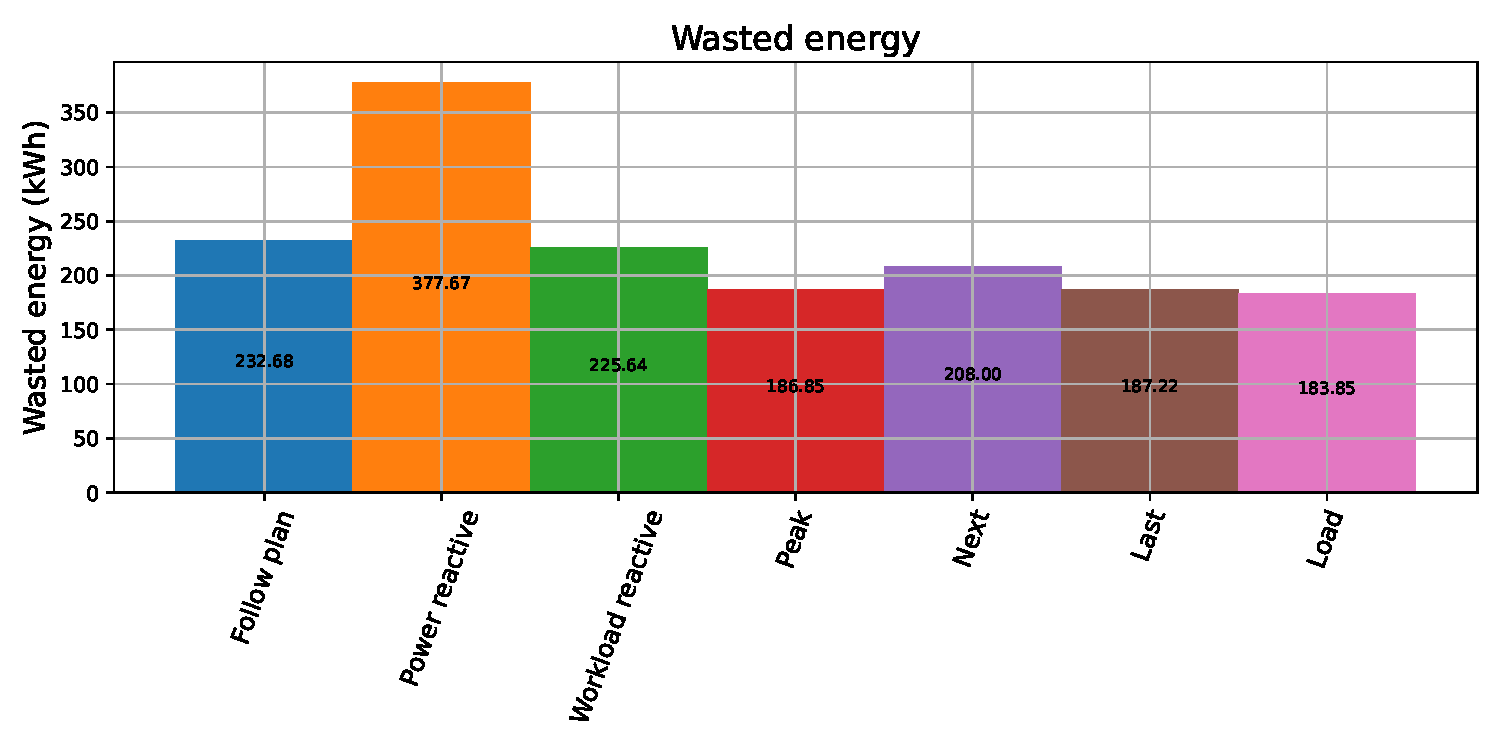
\includegraphics[scale=0.55]{Images/Compensations/energy_critical_4.pdf}
    \caption{Wasted energy at scenario critical 4.}
    \label{fig:energy_critical_4}
\end{figure}

\begin{figure}[!htb]
    \centering
    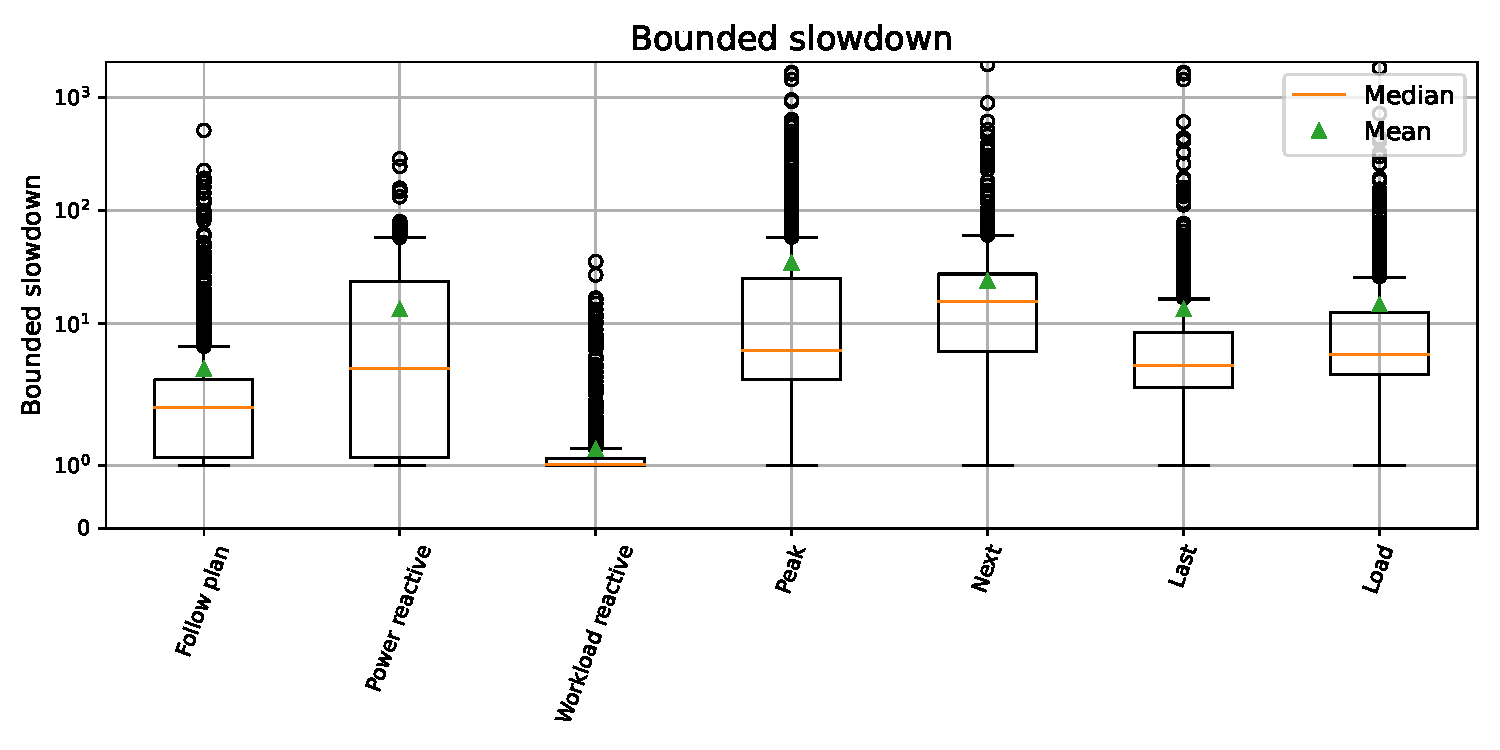
\includegraphics[scale=0.55]{Images/Compensations/slowdown_critical_4.pdf}
    \caption{Bounded slowdown at scenario critical 4.}
    \label{fig:slowdown_critical_4}
\end{figure}

The results in this scenario indicate that the policies degrade the QoS (finished jobs and slowdown) to appropriate the target level and QoS. The policies' compensation imposes the adaptations on power usage and server configuration. In this scenario, these adaptations demand a reduction of the number of available servers or reduce the speed of them. 

\clearpage

\subsection{Average cases}

After presenting the critical cases, this section demonstrates the results of 100 average cases. These average cases vary the power production and workload randomly, following a Gaussian noise. So, they are not always bad or good, like in critical scenarios. We do not present the slowdown in this scenario. The workload and power production vary a lot from one to another execution. So, it is inappropriate to compare them. First, Figure \ref{fig:SoC_diff} illustrates the state of charge difference from the target level. The red line is the target level. We can see that the three baselines (\emph{Workload reactive}, \emph{Power reactive}, and \emph{Follow plan}) have a big variance in the results. An important thing to notice is that even in not critical scenarios, the minimal values of \emph{Workload reactive} and \emph{Power reactive} can arrive at -30\%. This value means that these algorithms finished with the battery level at 20\%, which is the $SoC_{min}$. \emph{Follow plan} finishes with the higher Median and Mean, indicating that it saves more energy than the other algorithms. However, it also has a large variance.

\begin{figure}[!htb]
    \centering
    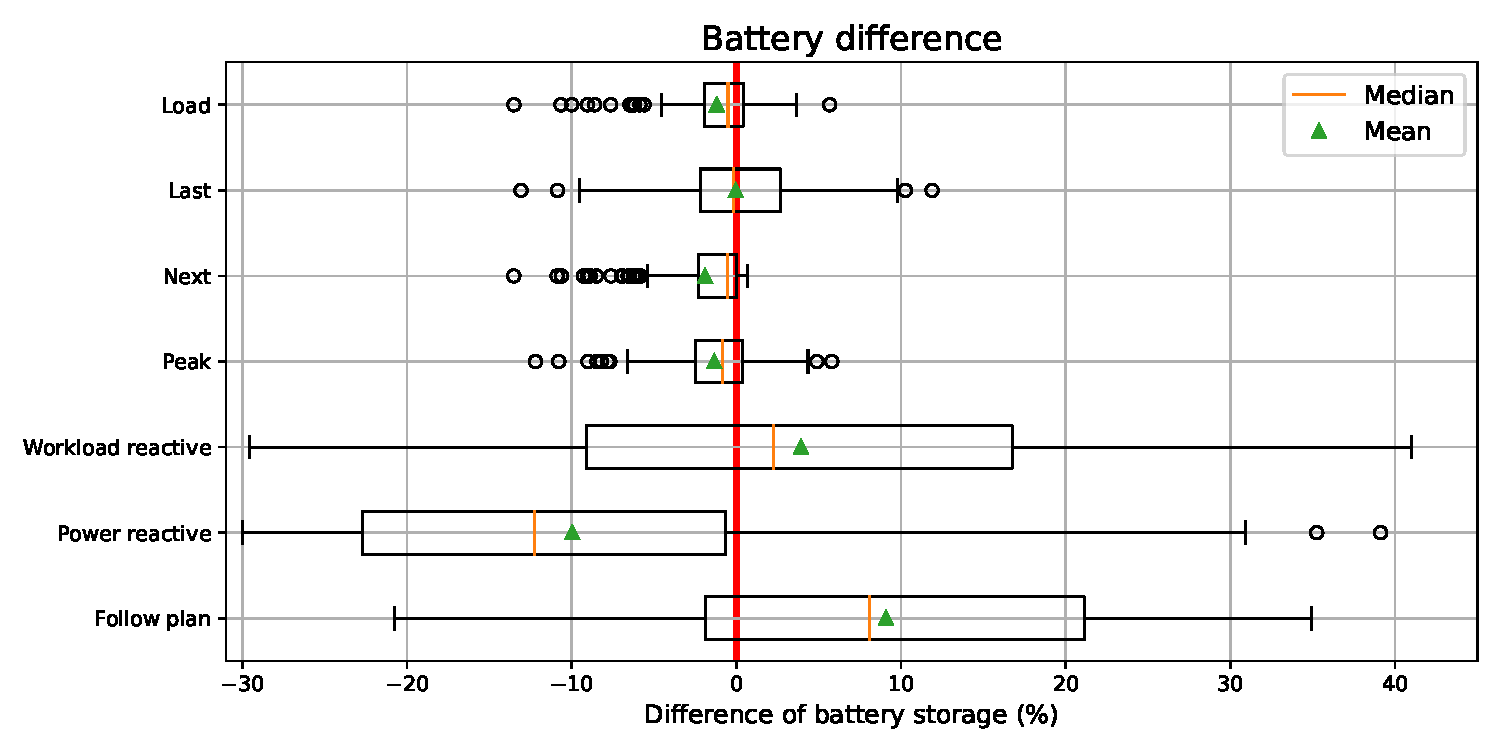
\includegraphics[scale=0.55]{Images/Compensations/battery_diff.pdf}
    \caption{Difference between the battery target level (50\%) and the real battery level at the end of the time window at 100 average cases. The line shows the standard deviation.}
    \label{fig:SoC_diff}
\end{figure}

The policies maintain the State of Charge between -10\% and 10\%, with some outliers below/above these values. The median and mean are very close to the target level, showing they can approximate the target level, which is the main objective of them. Last has the larger variance among the policies, but with median and mean almost perfect. This heuristic compensates in the last moments. Sometimes, this behavior can reduce the possibility to use the energy, since the heuristic will not have enough time. 

Regarding the QoS, Figures \ref{fig:finished_diff} and \ref{fig:killed_diff} illustrate the finished jobs and killed jobs. \emph{Workload reactive} has the best percentage of finished jobs (considering the number or size). This result is expected since this algorithm uses entirely the battery to maximize the number of finished jobs. \emph{Workload reactive} has also very low median and mean killed jobs. However, concerning the number of killed jobs, it has some results higher than 15\% (with two higher than 20\%). \emph{Power reactive} also has good finished jobs, but it never finished more than 97.90\%. This algorithm also has some executions with more than 15\% of killed jobs in number. The worst execution is \emph{Follow plan}, with a very high mean and median killed jobs (in number and size), and a very low finished jobs in size. Combining the state of charge from Figure \ref{fig:SoC_diff} with this result, we can notice that \emph{Follow plan} misses opportunities of using more power to execute more jobs or maintain big jobs running.

\begin{figure}[!htb]
    \centering
    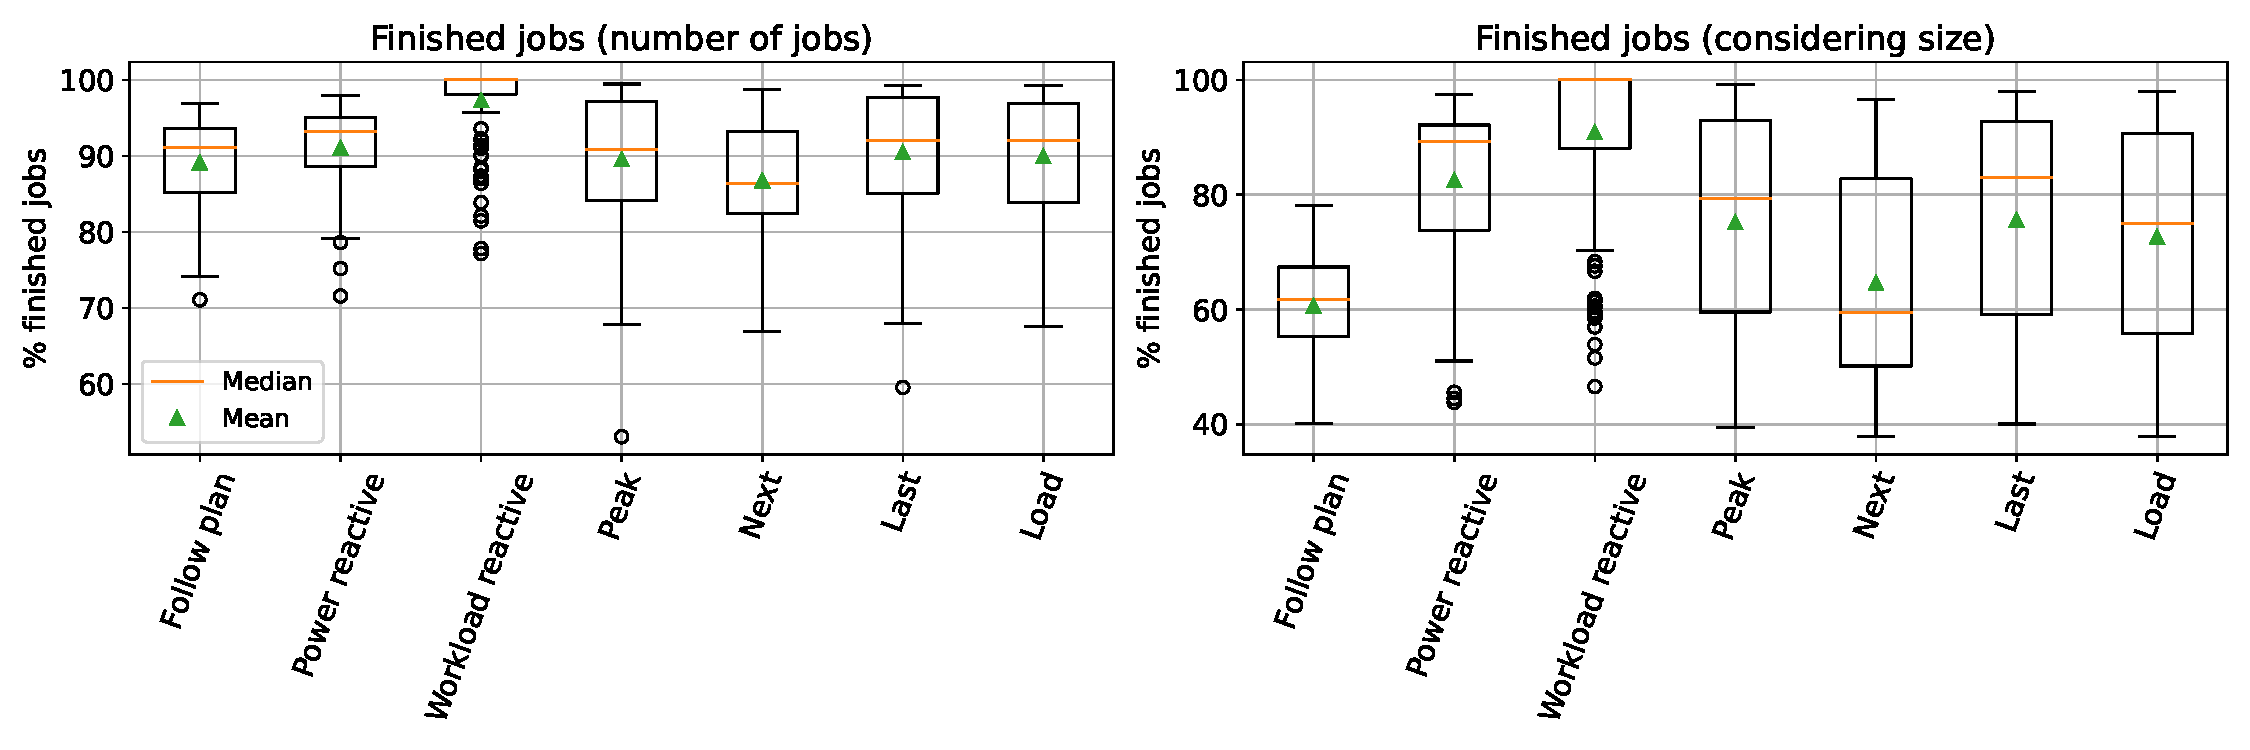
\includegraphics[scale=0.38]{Images/Compensations/finished_diff.pdf}
    \caption{Finished jobs at 100 average cases.}
    \label{fig:finished_diff}
\end{figure}

\begin{figure}[!htb]
    \centering
    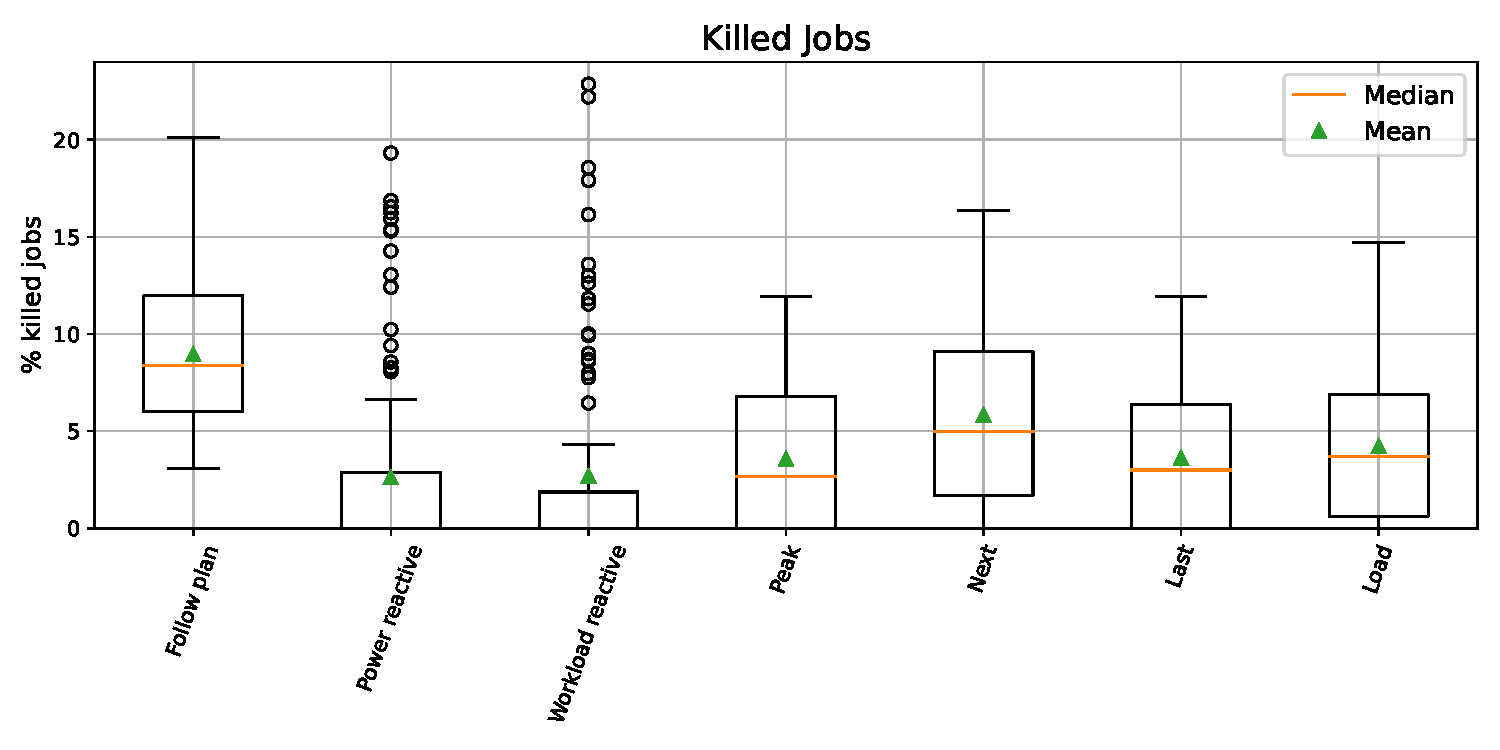
\includegraphics[scale=0.38]{Images/Compensations/killed_diff.pdf}
    \caption{Killed jobs at 100 average cases.}
    \label{fig:killed_diff}
\end{figure}

The policies have good finished jobs (in number), with \emph{Last} being a little below the \emph{Power reactive}. They also have some executions with almost 100\% of finished jobs (above 99\%). Considering the number of jobs killed, \emph{Last} and \emph{Peak} maintain the results in control, with no value above 15\%. \emph{Load} has the worst case close to 15\% and \emph{Next} with 16.37\%. Considering the size, the policies have worst results than \emph{Power reactive} and \emph{Workload reactive}. These jobs are harder to maintain running because they demand more time and power. So, the policies can kill them to guarantee the battery target level.

Finally, Figure \ref{fig:energy_diff} illustrates the wasted energy over 100 executions. The best execution is \emph{Workload reactive}. As mentioned before, this heuristic focus on running jobs, letting the servers down until they are needed. Also, the DPM technique reduces wasted energy. The worst algorithm is \emph{Power reactive}. This algorithm turns on servers even if they are not necessary. \emph{Follow plan} is better than three policies (\emph{Peak}, \emph{Next} and \emph{Load}). The best policy is \emph{Last}, mainly because it runs more jobs than the other policies and \emph{Follow plan}. While \emph{Follow plan} uses only the energy planned, the policies can reintroduce the energy from power variations. However, these policies change the usage using simplified heuristics. So, they can place the energy in moments without jobs to run. \emph{Last} is the policy that suffers the least from this problem because it places the compensations in the end. Therefore, it can re-migrate this energy at any moment before the end. Section \ref{sec:compensation_discussion} presents an overview of the advantages and problems of these policies. 

\begin{figure}[!htb]
    \centering
    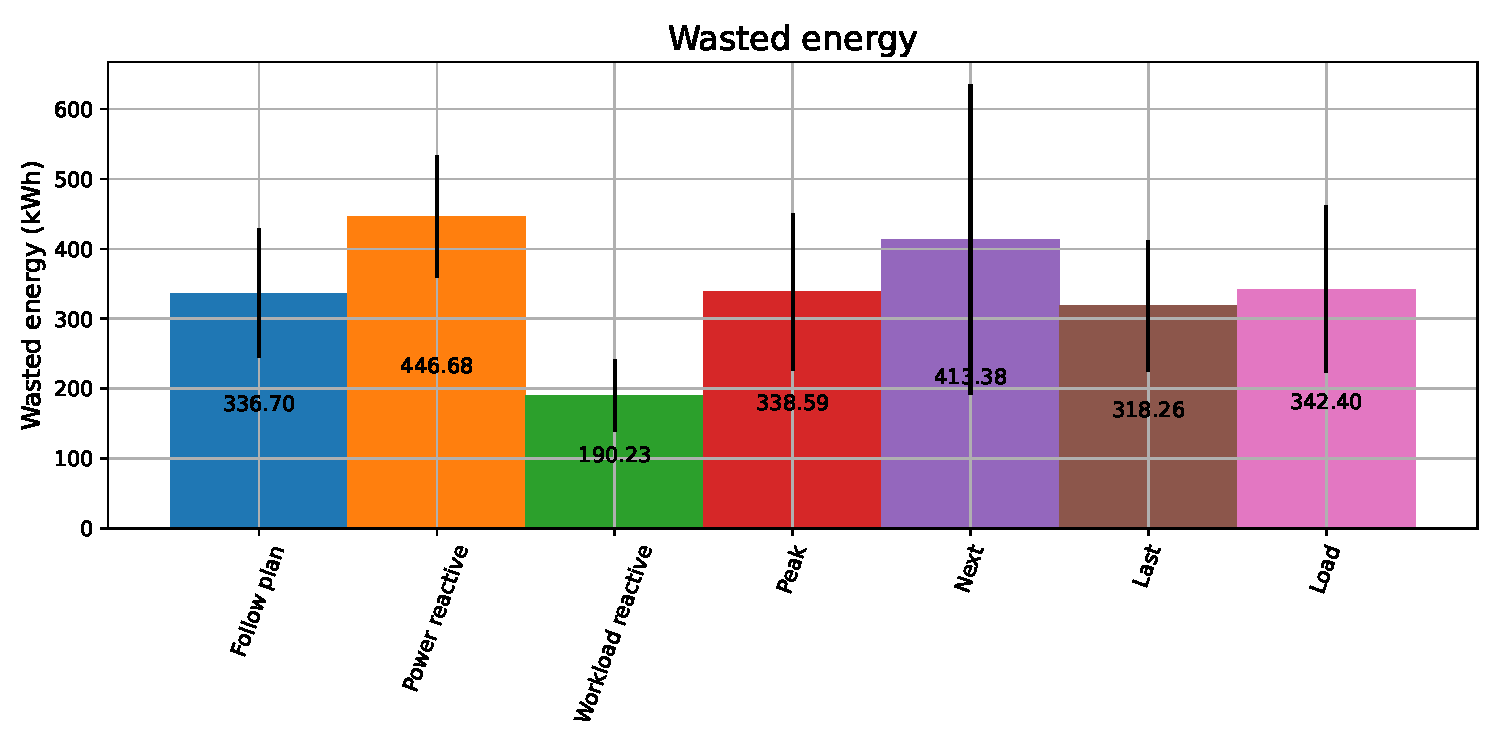
\includegraphics[scale=0.55]{Images/Compensations/energy_diff.pdf}
    \caption{Wasted energy at 100 average cases.}
    \label{fig:energy_diff}
\end{figure}

\clearpage

\subsection{Discussion}
\label{sec:compensation_discussion}

After presenting all results, this section discusses them generally. We highlight the pros and cons of all algorithms. Finally, we detail the gaps in the four policies that the following sections explore. The first algorithm is \emph{Follow plan}. This algorithm does not react to real events, applying the offline plan with no modifications. The results show that this approach tends to kill big jobs. Since the workload is composed of several small jobs (see Figure \ref{fig:metacentrum}), it can finish several jobs by number but not so much considering their size. Figure \ref{fig:jobs_critical_4} illustrates this case, where the algorithm finishes 85.48\% jobs considering the number, but only 57.70\% considering the size. In average cases, it also happens, where it finishes more than 90\% of the jobs in number but just more than 60\% in size (considering the median). In scenarios with more energy, \emph{Follow plan} does not use this energy to run more jobs. So, it saves energy but kills several jobs. This behavior can lead to high wasted energy, like in critical scenario 1 (see Figure \ref{fig:energy_critical_1}). Since \emph{Follow plan} does not adjust the plan, it finishes with more energy in the battery in cases with higher energy and with less energy in the battery in cases with less energy. The 100 average cases show that the minimal value is close to -20\% and the maximum value is above 30\%. These results highlight the importance of plan adaptations.

Then, a question comes up: Why not use fully reactive algorithms? Then, we presented \emph{Power reactive} and \emph{Workload reactive}. \emph{Power reactive} adapts the servers' speed according to the power available from renewable. It uses the battery to maintain a server available if the incoming renewable production is not enough. In every scenario, \emph{Power reactive} finishes with a very low battery level, even in the scenarios with more energy incoming from renewable. This algorithm only recharges the battery if the incoming renewable is not used by the servers (e.g., a server stays idle). However, it is not enough. Another problem in \emph{Power reactive} is the wasted energy. It has the worst results in every scenario. Since it does not use an offline plan, it losses a lot of energy in transition states. For example, if in a step the energy is high, it will turn on some servers. Nevertheless, if the energy drops in the next step, it turns them off. So, it wasted energy just reacting to the power available.

\emph{Workload reactive} is a very good algorithm from the QoS point of view. Considering the slowdown, for example, jobs do not wait too long to be placed (in an optimistic scenario). Also, it can finish more jobs than the other algorithms (see Figure \ref{fig:jobs_critical_2}). However, it can be too aggressive. In critical scenarios 1 and 3, it kills several jobs due to poor battery management. Figure \ref{fig:DPM_soc} illustrates that \emph{Workload reactive} places all the incoming jobs on the first day, dropping the battery level too fast. When SoC arrives at 20\%, \emph{Workload reactive} turns off all servers, killing several jobs and increasing the slowdown. This also happens in critical scenario 3, even if it receives more energy. In critical scenarios 2 and 4, it finishes with less energy than the target. In average scenarios, the final battery level of \emph{Workload reactive} varies a lot, going from -30\% to more than 40\%. So, this algorithm has poor battery management, like \emph{Power reactive}. Even if it seems appropriate to use the battery to maximize the number of finished jobs, the next time window will not have energy in the batteries to use. Therefore, both reactive algorithms are not viable for a renewable-only data center.

So, we proposed four policies to adapt power usage, mixing the offline plan with reactiveness. In general, \emph{Peak}, \emph{Next}, \emph{Last}, and \emph{Load} fulfill their main objective which is to finish the battery level as close as possible to the target level. In the profile worst-case scenarios (3 and 4), they degrade the QoS to approximate the battery level to the target. They do it by reducing power usage. On the other hand, they use the surplus energy from scenarios with profile best-case (1 and 2) to run more jobs. In scenario 1, they are even better than the \emph{Workload reactive}. Regarding the average cases, the policies finished very close to the target level. To do so, they impact the total finished jobs but have a more controlled number of killed jobs than the baselines. For example, \emph{Last} never killed more than 12\% of the jobs (considering the number of jobs). Therefore, these experiments show the impact on QoS of respecting the battery level.

It is difficult to indicate the best policy. \emph{Last} policy is the best one in critical scenarios 1 and 2. It finishes more jobs in number and size in critical scenario 1, and it is the second best in critical scenario 2. These scenarios have more energy, so \emph{Last} puts the positive compensations in the last step. When it needs to use more energy to maintain servers running, it takes the energy from the same (last) step. So, it is more likely for \emph{Last} to use the surplus energy. The drawback of \emph{Last} policy is that the last step can be too late to use the energy (see Figure \ref{fig:SoC_critical_1}), and it can miss opportunities to turn on servers to run more jobs. For example, \emph{Load} has a better slowdown than \emph{Last} in critical scenario 1 (see Figure \ref{fig:slowdown_critical_1}). \emph{Load} turns on servers in the moments where they are needed. So, when the jobs arrive, servers are waiting for them. \emph{Load} is the second best in scenarios 1 and 2. With more energy, it puts energy in the steps with a higher deficit between production and demand. However, the prediction is not perfect, and it can miss some steps. \emph{Next} has the worst results in these scenarios because it uses the surplus as soon as possible. Therefore, when it increases power usage, it is more complicated to find energy in future steps. Finally, \emph{Peak} has a balanced result in scenarios 1 and 2. It tends to maintain a more constant number of servers available over the steps. 

Regarding critical scenario 3, \emph{Next} and \emph{Peak} are good. In this scenario has less energy. Therefore, \emph{Next} adapts as soon as possible the usage. \emph{Peak} reduces the usage peak, maintaining a more stable usage. The behavior of both policies helps to avoid the lower battery boundary, without starting too many jobs that can not be finished. \emph{Load} is too aggressive here, dropping the SoC too fast and killing several jobs. Here, \emph{Last} is not so good. It does not adapt the usage on the first day, arriving faster at SoC lower boundary. Regarding the last critical scenario, \emph{Peak} is the best one among the policies. It has the lowest killed jobs (in number and size) among the policies. \emph{Next} has a good number of finished jobs, but a high number of killed jobs. Considering the size, it has the worst percentage of finished jobs. \emph{Load} is still aggressive, finishing fewer jobs (in number). \emph{Last} is a little better in this critical scenario, compared to the previous one. However, it still kills several jobs (second-worst among the policies). 

Finally, considering the 100 average cases, \emph{Last} finishes more jobs in number and size. \emph{Peak} and \emph{Load} are close, with \emph{Next} being the worst one. Comparing killed jobs, \emph{Last} and \emph{Peak} killed fewer jobs than \emph{Next} and \emph{Load}. \emph{Load} is too aggressive and \emph{Next} compensates too soon. Considering all these results, we can say that: 
\begin{enumerate}
    \item \emph{Last} policy is the best one when we have more power arriving. Let the power in the end, helps to migrate a second time when needed;
    \item \emph{Peak} policy has a good overall result, independent of the power profile;
    \item \emph{Next} is good in a context where the production is lower and it has a demand peak on the first day. In this scenario, the SoC drops too fast;
    \item \emph{Load} is aggressive, which pays off in slowdown, but can lead to several killed jobs.
\end{enumerate}

Regarding wasted energy, \emph{Next} is more likable to waste more than the other policies. It reintroduces the surplus as soon as possible, even if it is not necessary. \emph{Last} uses the energy wisely, since it places at the end, using before if necessary. \emph{Peak} and \emph{Load} depend on the scenario. Then, a new question comes up: Is it possible to improve the Quality of Service in these scenarios, while still respecting the battery level at the end of the time window? To do so, we first tried to mix the policies. For example, we can use \emph{Load} a little bit in positive compensations to improve QoS, then use \emph{Last} for the remaining energy surplus. We applied reinforcement learning to find out which policy to use at each moment. We present it in Chapter \ref{cha:learning_power_compensations}. 

\section{Conclusion}
This chapter proposed new heuristics to approximate the battery storage level to the target level. They use surplus energy to improve the QoS, mainly the finished jobs. The policies try to reduce the impact on QoS in scenarios with less energy. The following chapter takes a step further, trying to mix the policies, aiming to improve QoS even more.

    \chapter{Learning Power Compensations}

\section{Introduction}

\section{Algorithms}

\subsection{Random}

\subsection{Q-Learning approach}

\subsection{Contextual Multi-Armed Bandit approach}

\section{Results Evaluation}

\section{Conclusion}

    \chapter{Adding Battery Awareness in EASY Backfilling}
\label{cha:heuristic}

\minitoc

\section{Introduction}

After trying to introduce reinforcement learning in our model to choose the best compensation policy, this chapter describes a heuristic that englobes several elements to make better decisions. We named this heuristic \emph{\systemName} (Battery EASY backfilling). This heuristic considers the power production and demand to find the best moment to compensate. In addition, \emph{\systemName} mixes the compensations with the scheduling decisions. We present the algorithm, followed by the results compared with the previous heuristics.

\section{\systemName}

This heuristic acts in three different moments. First, Section \ref{sec:model_predictions} explains the predictions used through \emph{\systemName}'s decisions. These predictions are made at the beginning of the time window, just one time. Then, Section \ref{sec:model_easy} describes the modifications in the EASY Backfilling heuristic to introduce battery awareness. The modified EASY Backfilling acts every time a job finishes, arrives, or new servers are available. Finally, Section \ref{sec:model_compensations} defines the compensation policies. \emph{\systemName} compensates every time step.

\subsection{Predictions}
\label{sec:model_predictions}

As presented in Section \ref{sec:offline_plan}, ODM receives two predictions from offline modules: power production and power demand. Since ODM works online, it will not predict itself but use the predictions from offline. So, this section will not focus on the forecasting method but on using its results.

\begin{figure}[!htb]
    \centering
    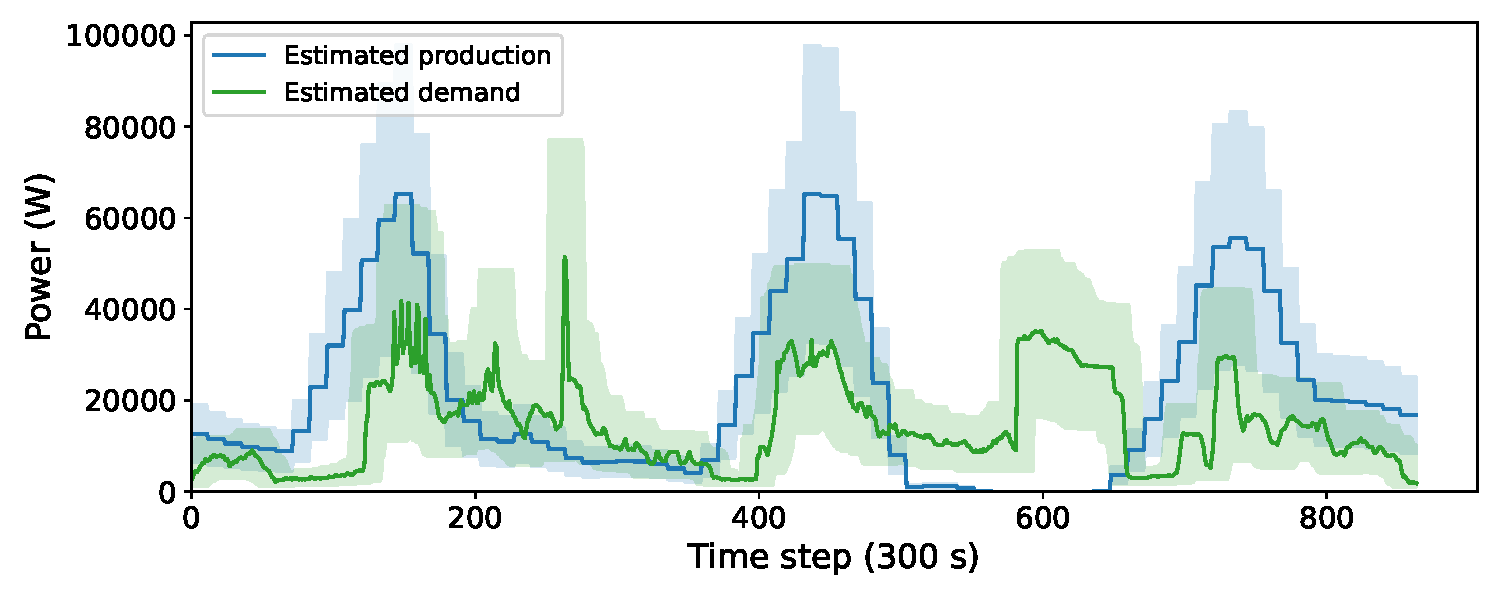
\includegraphics[scale=0.5]{Images/Heuristic/predictions.pdf}
    \caption[Renewable production and demand prediction.]{Renewable production and demand prediction. The blue (production) and green (demand) areas are the uncertainty given by the forecast.}
    \label{fig:predictions}
\end{figure}

Figure \ref{fig:predictions} illustrates both forecasts showing the area of uncertainty. The real value can be any value inside the uncertainty area. \emph{\systemName} uses these predictions to create different possible states of charge using equations \ref{equ:battery_energy} and \ref{equ:battery_state_of_charge}. To do so, we estimated $P_{dch}$ and $P_{ch}$ using Equations \ref{equ:battery_charge}, and \ref{equ:battery_discharge}: 
\begin{equation}
    \label{equ:battery_charge}
    P_{ch}(t) = 
    \begin{cases}
        P_{renew}^{est} - P_{load}^{est},& \text{if } P_{renew}^{est} > P_{load}^{est} \\
        0,              & \text{otherwise}
    \end{cases}
\end{equation}
\begin{equation}
    \label{equ:battery_discharge}
    P_{dch}(t) = 
    \begin{cases}
        P_{load}^{est} - P_{renew}^{est},& \text{if } P_{renew}^{est} < P_{load}^{est} \\
        0,              & \text{otherwise}
    \end{cases}
\end{equation}

Where:
\begin{itemize}
    \item \(P_{renew}^{est}\): Estimated power production from renewable;
    \item \(P_{load}^{est}\): Estimated power demanded from the load.
\end{itemize}

\begin{figure}[!htb]
    \centering
    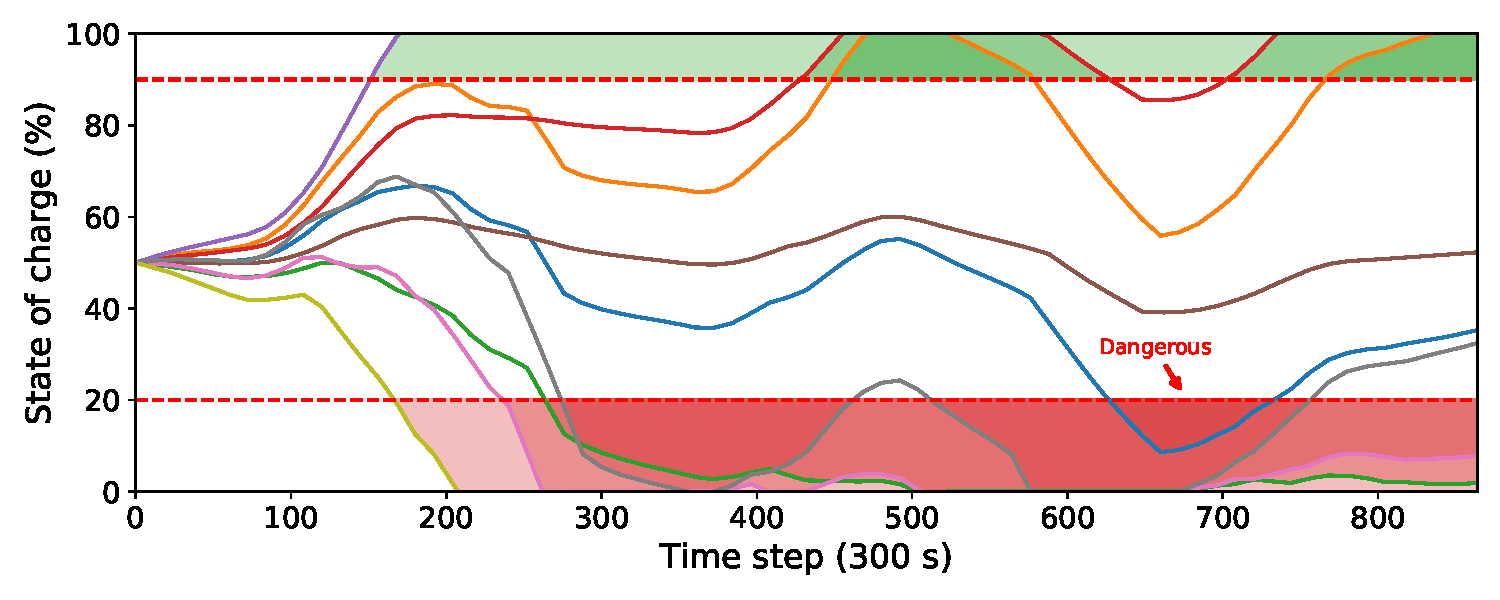
\includegraphics[scale=0.5]{Images/Heuristic/state_of_charge.pdf}
    \caption[Result of the Equation \ref{equ:battery_state_of_charge} for different predictions.]{Result of the Equation \ref{equ:battery_state_of_charge} for different predictions. The dangerous area is when 5 or more curves (so, more than half of them) are below 20\%.}
    \label{fig:estimated_state_of_charge}
\end{figure}

Figure \ref{fig:estimated_state_of_charge} demonstrates the result of estimating the SoC (with Equation \ref{equ:battery_state_of_charge}) using nine different predictions. \emph{\systemName} calculates these SoC combining lower, median, and upper boundaries from the area presented in Figure \ref{fig:predictions} (e.g., demand lower boundary + production lower boundary, demand median + production lower boundary, demand median + production higher boundary, etc...). It is possible to notice that the SoC can vary a lot. Section \ref{sec:model_compensations} will describe how we use these SoCs to compensate. Figure \ref{fig:estimated_state_of_charge} also illustrates both SoC upper and lower thresholds (red dashed lines). Setting upper and lower thresholds helps to increase the battery lifetime \cite{xu2016modeling}. The narrower the range, the longer the expected lifetime \cite{xu2016modeling}. However, selecting a narrow range limits the battery benefits. The figure presents both thresholds as 90-20\%, but they are parameterizable. Finally, \emph{\systemName} estimates dangerous areas in the time window. Figure \ref{fig:estimated_state_of_charge} indicates this moment. It considers the dangerous areas when more than half of the predicted SoC curves are below the lower threshold (in Figure \ref{fig:estimated_state_of_charge}, 5 curves). Section \ref{sec:model_easy} will explain how it uses these moments to make better scheduling decisions. The opposite is the green areas, where the battery will be overcharged. In these moments we could use more energy from the batteries to stay below the thresholds. However, just expending energy without need will increase the wasted energy. So, \emph{\systemName} focuses on using the energy efficiently (detailed in Section \ref{sec:model_compensations}). 

\subsection{Job Scheduling}
\label{sec:model_easy}

One of the most important ODM's duties is placing jobs on servers. To do so, \emph{\systemName} implements EASY backfilling using two different sorts \cite{mu2001utilization, lelong2018tuning}. Algorithm \ref{alg:algo_scheduling_heuristic} presents the main idea. This algorithm is similar to Algorithm \ref{alg:algo_scheduling} but with some modifications (we highlighted them). \emph{\systemName} runs this algorithm when a job arrives, finishes, or new servers are available. First, this heuristic defines the priority order (line 2) and sorts the jobs in the queue in a priority order $P_{R}$ (line 3). We explain later how it defines the priority order. Then, it finds the servers to run this job (line 6). The server must be available at least at the actual time step to be chosen. Line 7 has the first modification. Usually, EASY backfilling only verifies if servers $S$ are available now. We added the following verifications:

\begin{enumerate}
    \item It verifies if servers $S$ are available during the entire execution, considering the walltime given by the user as the execution time. If so, it returns true. If not, it goes to the next verification;
    \item It verifies if it is possible to change the plan to keep servers S running the entire execution. To do so, it does the following steps:
    \begin{enumerate}
        \item First, it calculates how much energy is needed. Let's say $Ed_t$ is the energy demanded in step $t$ without modification and $Ed_t^{'}$ is with modification. So, it calculates $Ed_t^{'}$ for each time step $t$ that the server sleeps, putting the server in the same state/speed as the previous time step ($t-1$). The total energy demanded is $\sum_{t} Ed_t^{'} - Ed_t$ considering all the time steps that the job executes;
        \item Then, it calculates how much energy is possible to take from future steps, putting idle servers to sleep. Let it be $E_{poss}$. Since we need to maintain the SoC between both thresholds, we can not "migrate" all the energy to use now. So, it only considers the idle servers from the actual time step until the time step where the SoC will be equal or lower to the lower threshold. We can migrate the energy freely between the actual time step and this future one. Figure \ref{fig:idle_machines_verification} illustrates this verification. In the figure's example, the actual step is at hour 10. In this step, it needs to verify how much energy is possible to save from future steps. So, it verifies the idle servers from hour 10 to hour 29, because at hour 30 the SoC is equal to 20\%. It can change the usage from hour 10 to hour 29 freely. Taking energy from after hour 30 could violate the lower threshold since we will use more energy from the batteries;
        \item Then, it tests if $E_{poss} >= \sum_{t} Ed_t^{'} - Ed_t$. If this is false, it returns false and does not change the plan. If this is true, it makes $Ed_t = Ed_t^{'}$, changes the server speeds, and recalculates the planned SoC (using Equation \ref{equ:battery_state_of_charge}).
    \end{enumerate}
\end{enumerate}

\IncMargin{1em}
\begin{algorithm}[!htb]
    \LinesNumbered
    \footnotesize
    \SetAlgoLined
    \SetKwInOut{Input}{input}\SetKwInOut{Output}{output}
    \Input{Queue $Q$ of waiting jobs, $P_{R}$ as priority order, and $P_{B}$ as backfilling order.}
    \Output{None (calls to \textit{Start()})}
    \Begin{
        $P_{R} \leftarrow$ \textit{define\_priority\_sort()}\;
        Sort $Q$ according to $P_{R}$\;
        \For{job $j$ in $Q$}{
            Pop $j$ from $Q$\;
            $S \leftarrow$ \textit{select\_servers($j$)}\;
            \uIf{\hl{$j$ can be started and finished in servers $S$}}{
                \textit{Start($j$, $S$)}\;
            }\Else{
                Reserve $j$ at the earliest time possible according to the walltime of the currently running jobs\;
                Sort $Q$ according to $P_{B}$\;
                \For{job $j^{'}$ in $Q$}{
                    $S \leftarrow$ \textit{select\_servers($j^{'}$)}\;
                    \If{\hl{$j^{'}$ can be started and finished in servers $S$ without delaying the reservation on $j$}}{
                        \textit{Start($j^{'}$, $S$)}\;
                    }
                }
                \textbf{break}\;
            }
        }
    }
    \caption{\emph{\systemName} scheduling. Modified from \cite{lelong2018tuning}.}
    \label{alg:algo_scheduling_heuristic}
\end{algorithm}
\DecMargin{1em}

\begin{figure}[!htb]
    \centering
    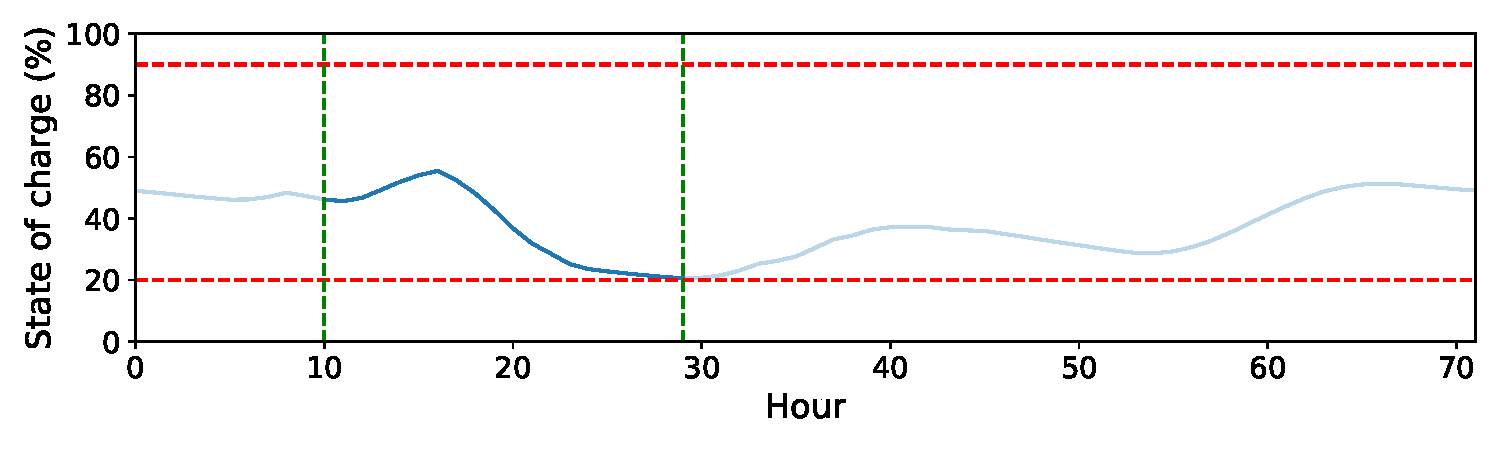
\includegraphics[scale=0.5]{Images/Heuristic/idle_machines.pdf}
    \caption{Verification of possible energy to save.}
    \label{fig:idle_machines_verification}
\end{figure}

These verifications do not increase the complexity. Verification 1 goes through the plan with limited size (e.g., in our three-day time window, we have a plan with 864 time steps). Verification 2-a is done together with verification 1. Verification 2-b is faster than the others since it can process fewer steps and stop when $E_{poss} >= \sum Ed_t^{'} - Ed_t$. Verification 3-c is just to apply the modifications. It recalculates the SoC to keep it updated for the next jobs to schedule. So, if a job puts a future SoC close to the lower threshold, the next job takes it into account. Continuing in algorithm \ref{alg:algo_scheduling_heuristic}, if the tests pass, then it starts the job (line 8). When it finds a job that can not be placed now, the algorithm does the backfill process (lines 10-18). Then, it finds the first moment to run this job (named priority job) in the future (line 10). So, it re-sorts the queue using $P_{B}$ (line 11), placing the other jobs in the servers (lines 12-17) without delaying the (future) priority job execution (line 14). Line 14 does the same verification as line 7.

As mentioned before, EASY backfilling sorts the jobs by $P_{R}$ and $P_{B}$. Line 2 defines $P_{R}$. Our implementation starts with $P_{R}$ using Bounded Slowdown from Equation \ref{equ:slowdown}. Bounded Slowdown estimates the ratio between the total time a job stays in the system and its actual processing time. This order helps to let a job wait proportionately to its size. For $P_{B}$, \emph{\systemName} sorts the waiting queue by the smallest sizes first (walltime multiplied by the number of resources needed). This order helps in the backfill process since sometimes the "holes" in the scheduling demand very small jobs. Besides, these jobs are less likely to demand more energy from future time steps (\emph{\systemName} lets the energy to the priority ones). Figure \ref{fig:estimated_state_of_charge} highlights a dangerous area. In this area, \emph{\systemName} changes $P_{R}$ to also use the smallest sizes first. These are not good moments to start big jobs, even if they are waiting too long in the queue. Small jobs demand less energy and are more likely to finish.

\subsection{Power compensation}
\label{sec:model_compensations}

After describing the scheduling algorithm, this section explains the heuristic to compensate for power fluctuations. While the scheduling algorithm runs for every job arrival, end, or server state modification, the power compensation algorithm will execute at every new time step. Since the scheduling algorithm modifies future time steps (it places the jobs in servers that are already on) and verifies the violations, we do not need to run the power compensations for every placement. We defined that the state and speed stay constant inside each time step. Changing the server state too much between on and off can degrade it faster. Besides, these transitions take time. Therefore, a constant state/speed inside time steps simplifies the decision-making.

The main objective of this part of the heuristic is to finish the time window with the SoC as close as possible to the planned. Renewable sources can produce more or less than predicted. Furthermore, the power usage can vary due to server idleness or scheduling modifications. So, at each time step, \emph{\systemName} calculates the SoC for all future time steps using Equation \ref{equ:battery_state_of_charge}. Then, it calculates the energy difference $E_{comp}$ between the target and the estimated SoC at the end of the time window using Equations \ref{equ:delta_energy} and \ref{equ:energy_battery}. \emph{\systemName} needs to reintroduce/remove the energy $E_{comp}$ before the end of the time window.

When the compensation is positive ($E_{comp}>0$), we can increase the speed of the servers or run more jobs. First, \emph{\systemName} uses the $E_{comp}$ to speed up the running jobs. It improves from the actual step until the last step. In each step, \emph{\systemName} increases the processor's speed of the running jobs on this step. So, it tends to put more energy into the jobs right now than in the future. This behavior helps in avoiding jobs to reach their walltime and also avoiding steps with predicted SoC higher than 90\%. After that, if there is still energy, it verifies if there are jobs in the waiting queue. If so, it turns on some servers to run these jobs. If there is not or it turned all the servers needed to run jobs, it lets the remaining energy in the battery. Expending the energy only by increasing job speeds and starting new jobs can be very conservative. Even so, these actions help to avoid the battery's higher threshold of 90\%. \emph{\systemName} could be aggressive, using the remaining energy to turn on machines in the future without knowing exactly if there will be jobs to execute. However, we prefer to finish with more energy in the batteries than expend this energy not wisely. Being aggressive can lead to a higher wasted energy. 

In the negative compensation ($E_{comp}<0$), \emph{\systemName} considers the estimated SoCs from Figure \ref{fig:estimated_state_of_charge}. First, it finds the time step with the higher number of predictions below 20\% or the last time step if there are no predictions below 20\% (let's name it the violation time step). The idea is to reduce the usage before the violation, reducing the violation probability. Then, \emph{\systemName} reduces servers speed in the following order (stopping when it is enough):
\begin{enumerate}
    \item Impacts idle servers from the violation time step to the actual time step (it goes through the time steps backward);
    \item Impacts idle servers from the violation time step to the last time step (it goes through the time steps forward);
    \item Impacts running servers from the violation time step to the last time step (it goes through the time steps forward);
    \item Impacts running servers from the violation time step to the actual time step (it goes through the time steps backward);
\end{enumerate}

\emph{\systemName} focuses first on idle servers because impacting running servers can increase the number of killed jobs. Killing jobs increases wasted energy. So, \emph{\systemName} searches for idle servers in both ways (violation time step $\rightarrow$ actual time step and violation time step $\rightarrow$ last time step). If reducing the usage from idle servers is insufficient, we start to impact running servers (steps 3 and 4). Our idea is to impact them as far as possible from the actual step, considering the violation step. The real total job execution time is uncertain (e.g., they could finish earlier than predicted). If we change the order (step 4 before step 3), the chance of really impacting the job is higher since it will reduce the energy from the violation step to the actual step. Doing step 3 before, we expect that the job finishes before these changes, while impacting the steps around the violation step. \emph{\systemName} kills jobs only when there is no power action possible (e.g., migrating power from the future) to keep them running. Aiming to avoid a blackout in the data center, we turn off the servers gently, killing the running jobs in the process. We do not focus on the killed jobs resubmission.

\section{Results Evaluation}

After presenting \emph{\systemName}, we compare its results with the algorithms presented previously. We execute the same critical cases and 100 random cases presented in Section \ref{sec:experiment_environment}. Just to remember, the critical cases are:
\begin{enumerate}
    \item \emph{Critical 1}: Profile best-case and workload in the beginning;
    \item \emph{Critical 2}: Profile best-case and workload in the end;
    \item \emph{Critical 3}: Profile worst-case and workload in the beginning;
    \item \emph{Critical 4}: Profile worst-case and workload in the end;
\end{enumerate}

The random cases are the 100 workloads and power productions generated by Gaussian noise over 10 different traces of each (workload and power production). The results of the baselines and policies are the same as the previous sections.

\subsection{Critical cases}

\subsubsection{Scenario Critical 1}

Figure \ref{fig:beasy_critical_1} illustrates all the results obtained for the execution with the profile best-case and workload in the beginning. This scenario has more space for improvement because the job majority arrives on the first day, and we have more energy to finish them than predicted. So, the heuristics have time to decide when to start the jobs and how to approximate the target SoC. The best algorithm is \emph{\systemName}, with 99.01\% finished jobs in number and 96.07\% size. The jobs not finished are postponed and not killed. It ends above the target SoC. Regarding wasted energy, it is possible to notice that \emph{\systemName} better expends the energy received, resulting in a saving of 35.33\% compared with the second-best wasted energy result (\emph{Workload reactive}). It has a higher bounded slowdown compared to the policies but a lower mean than the baselines. It runs more jobs, which makes more jobs wait longer. However, it maintains all slowdowns below 100, while all other algorithms have some jobs with higher slowdowns.

\begin{figure}[!htb]
    \centering
    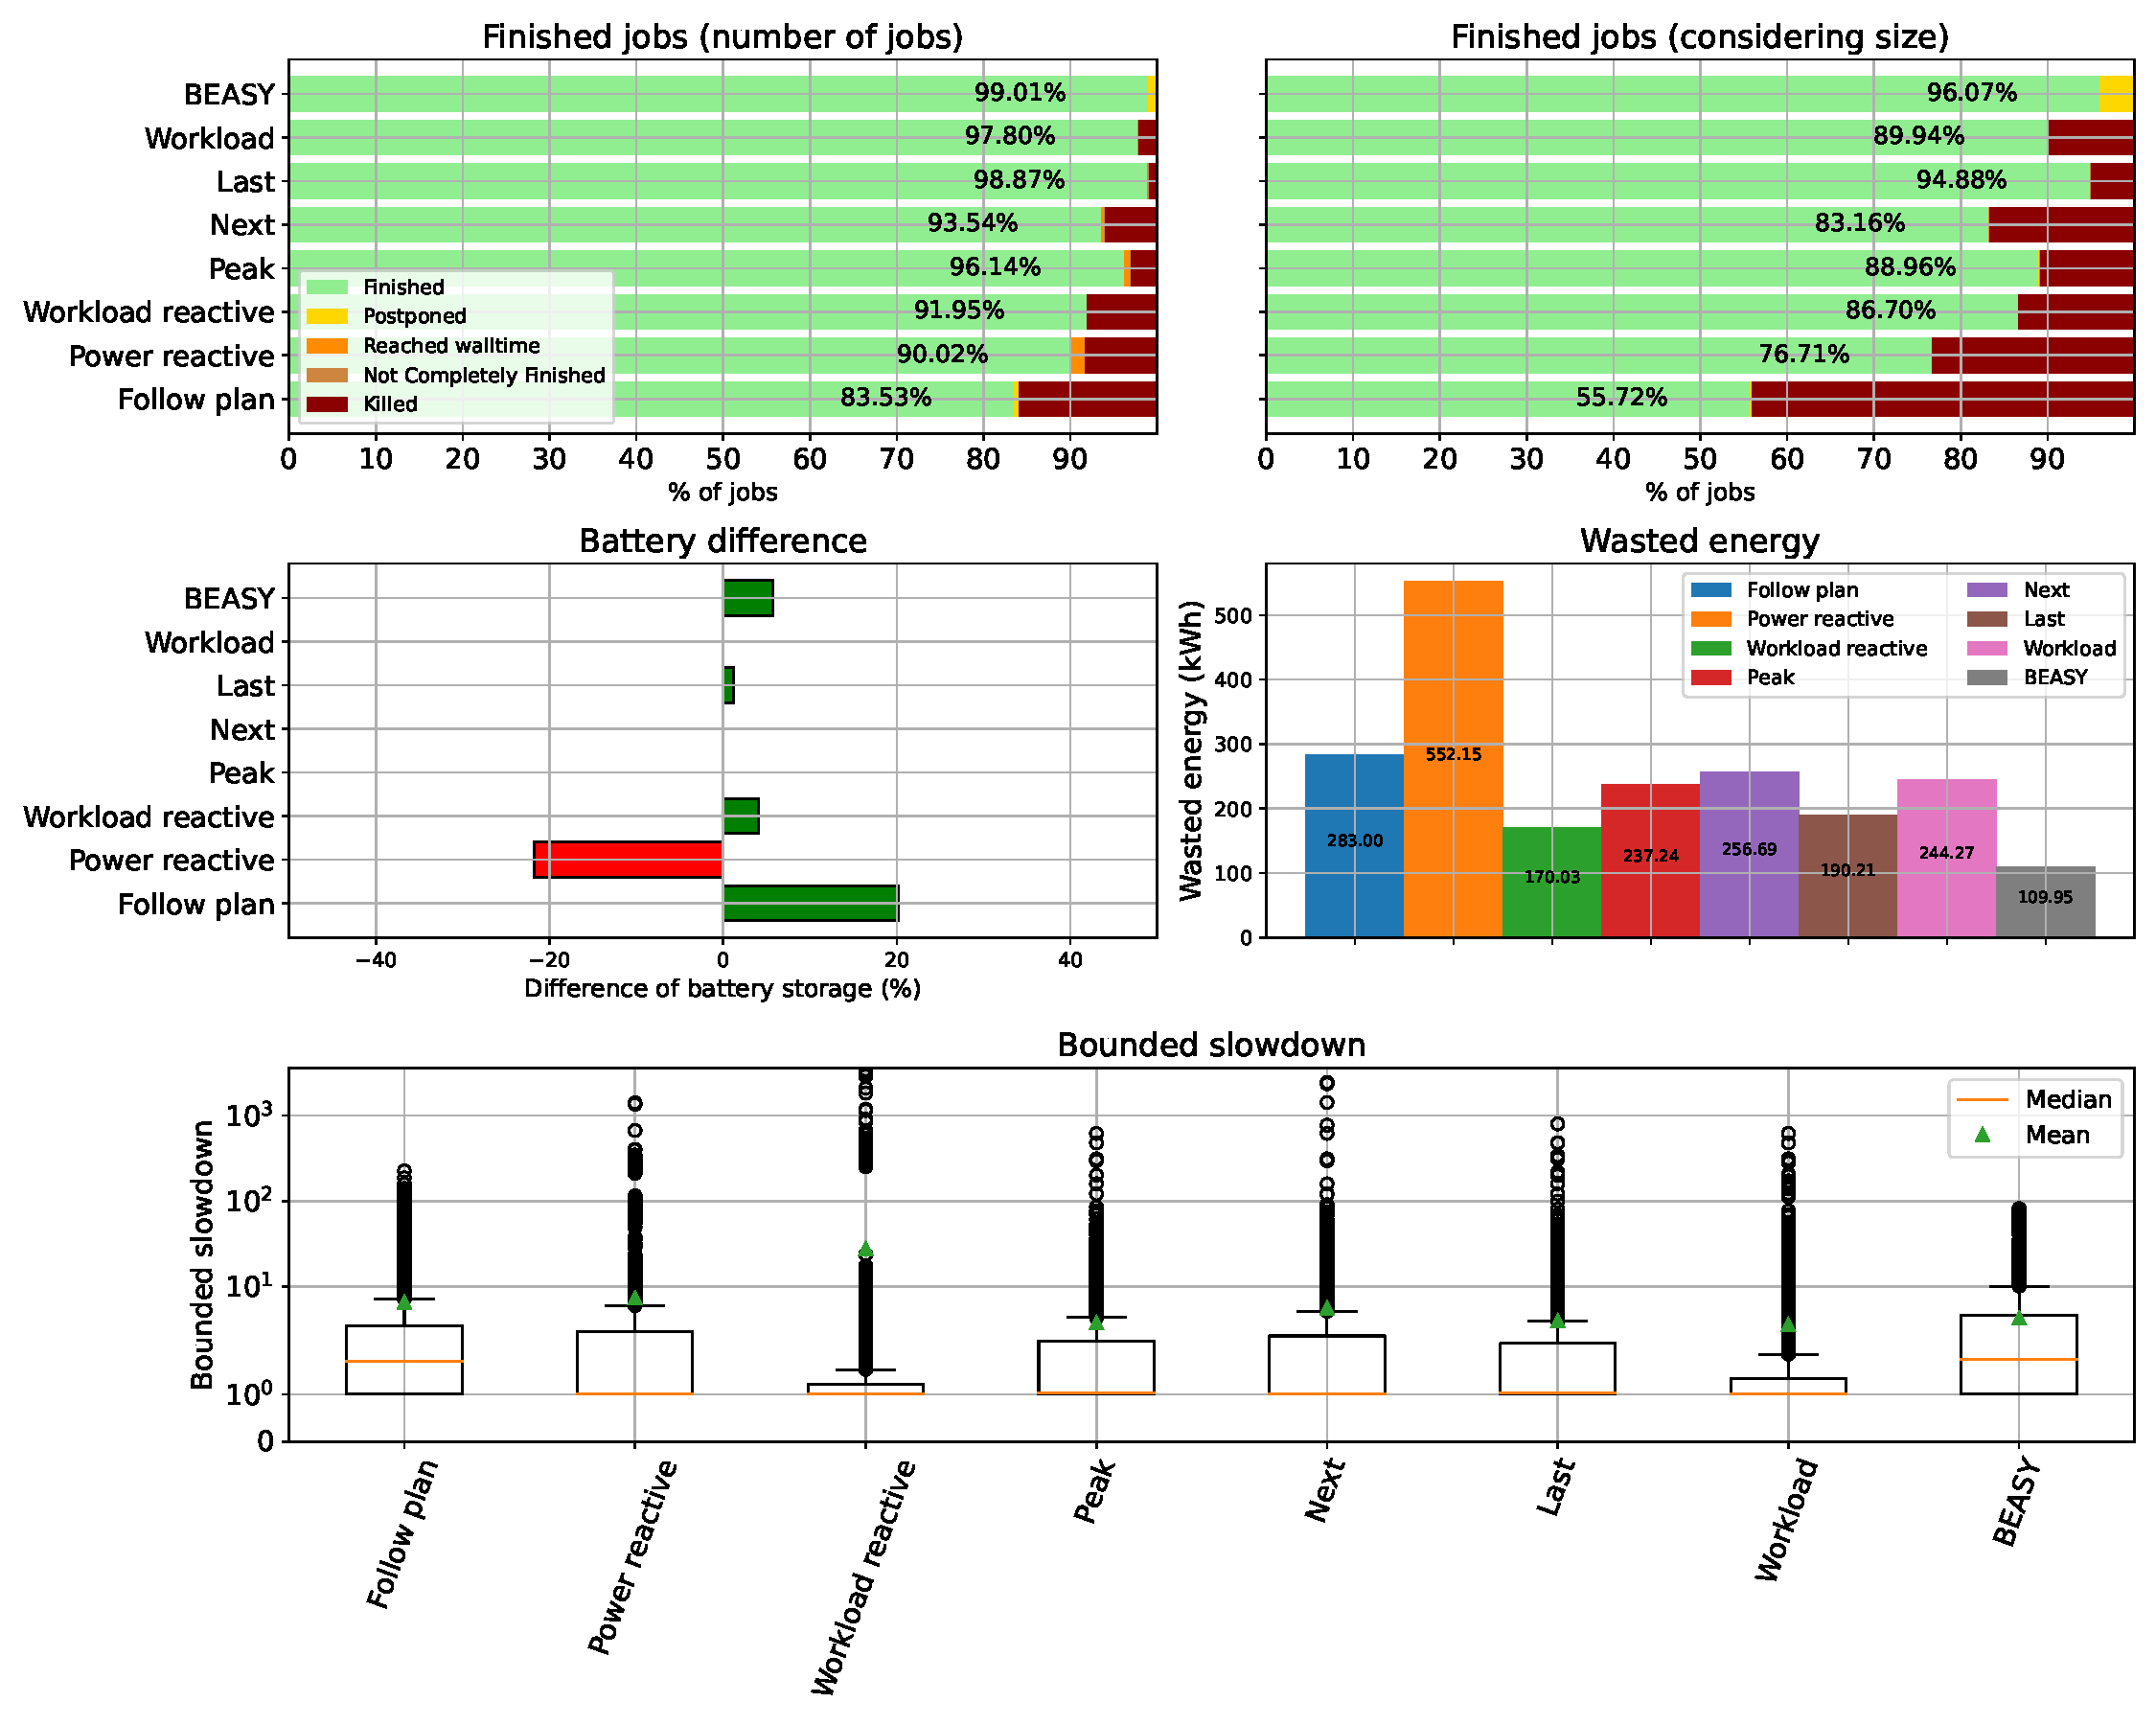
\includegraphics[scale=0.39]{Images/Heuristic/profile_best_workload_1_with_noise.pdf}
    \caption{Results of \emph{\systemName} on critical case 1.}
    \label{fig:beasy_critical_1}
\end{figure}

\emph{Workload reactive} execution kills 8.05\% of jobs. This heuristic is too aggressive compared to \emph{\systemName}. As mentioned before, \emph{Workload reactive} puts all jobs to start as soon they arrive. Figure \ref{fig:critical_soc_s1} compares the SoC of the \emph{Workload reactive} and \emph{\systemName}. \emph{Workload reactive} dries too fast the battery and needs to kill the jobs, while \emph{\systemName} is conservative. We can see in this scenario that \emph{\systemName} makes better decisions than all other executions. Here, being conservative helped in the result. It finishes more than 99\% of the submitted jobs, guaranteeing they have the energy to finish. The 1\% is postponed to the next time window. We discuss this approach later. In addition, it finishes saving energy in the battery, which can help the next time step to run the postponed jobs.

\begin{figure}[!htb]
    \centering
    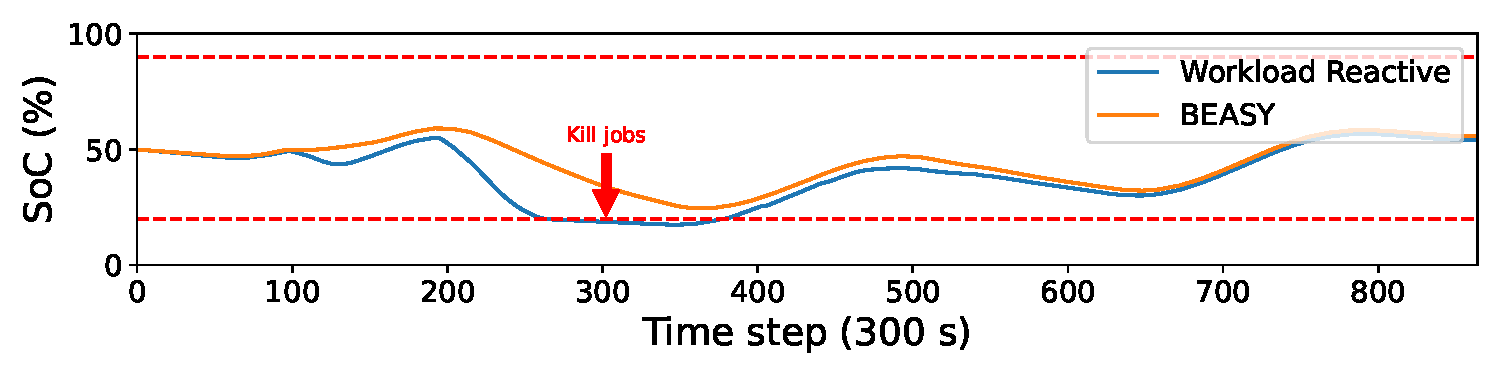
\includegraphics[scale=0.5]{Images/Heuristic/critical_soc_s1.pdf}
    \caption{Comparison between the SoC of \emph{Workload reactive} and \emph{\systemName}.}
    \label{fig:critical_soc_s1}
\end{figure}

% \clearpage

\subsubsection{Scenario Critical 2}

The second case is more complicated than the previous one. Here, the job majority arrives on the last day of the time window. So, the algorithms have a shorter time to schedule them. Figure \ref{fig:beasy_critical_2} illustrates the results. 

\begin{figure}[!htb]
    \centering
    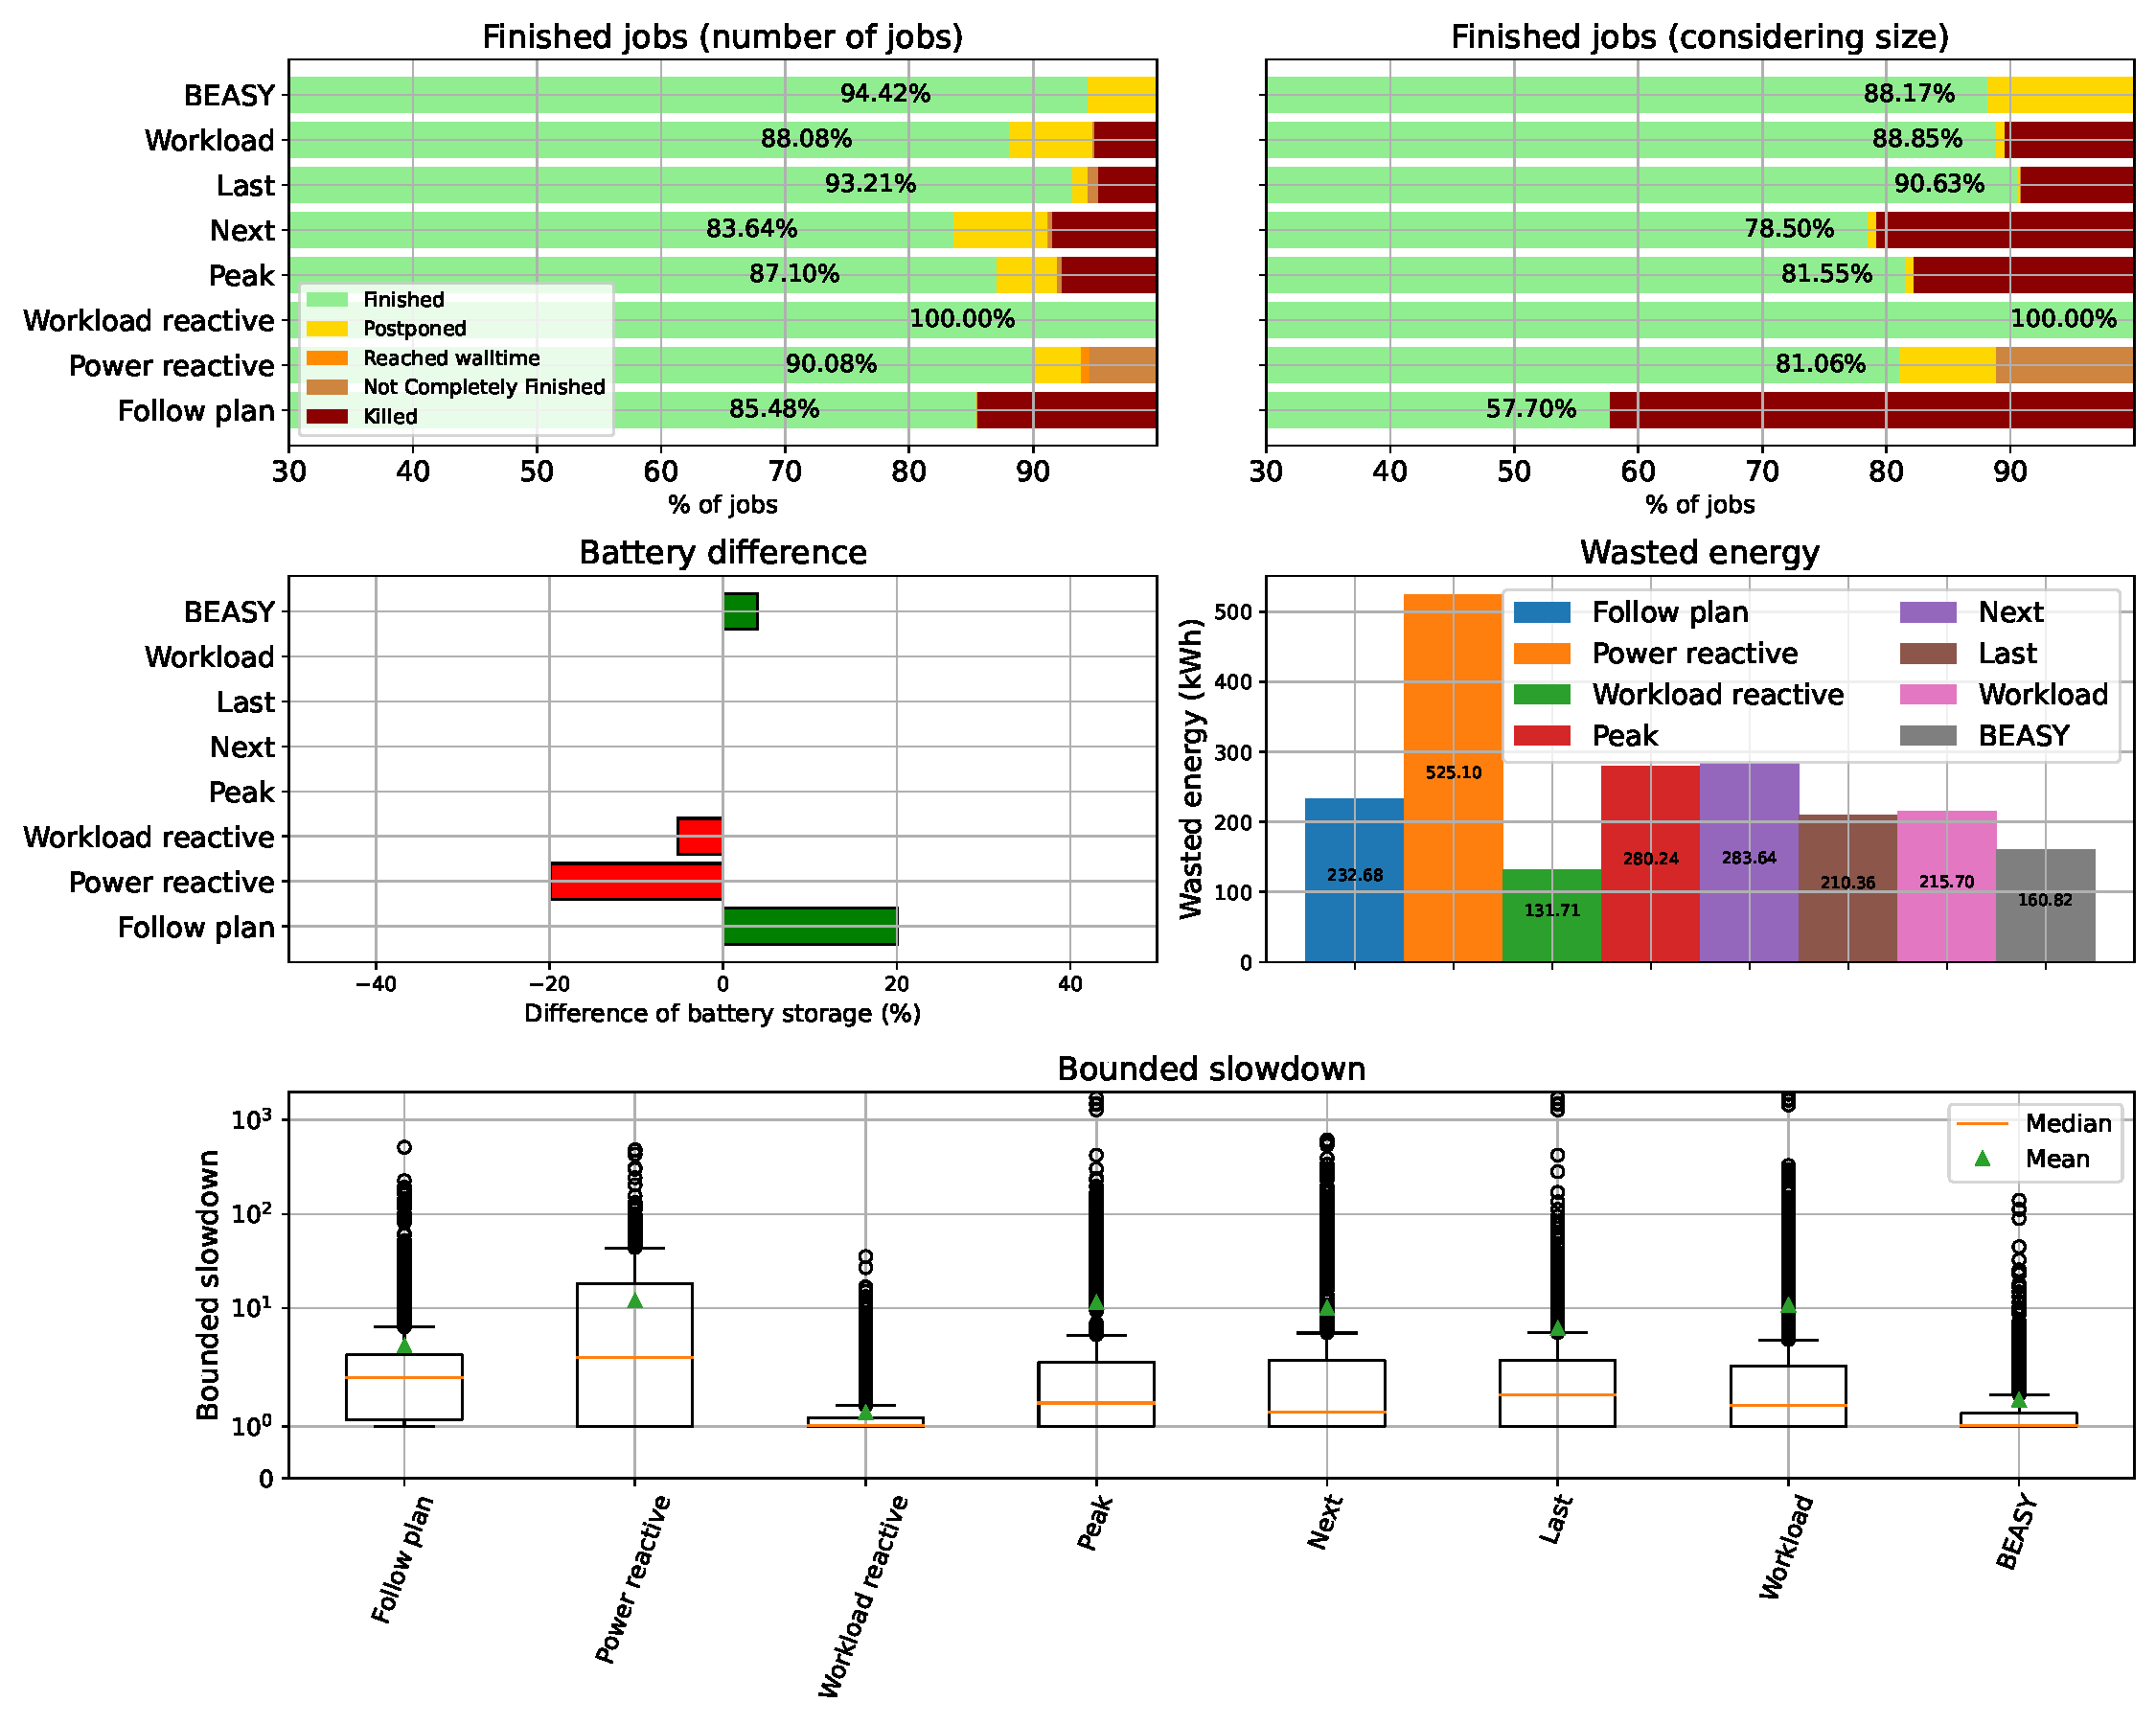
\includegraphics[scale=0.39]{Images/Heuristic/profile_best_workload_2_with_noise.pdf}
    \caption{Results of \emph{\systemName} on critical case 2.}
    \label{fig:beasy_critical_2}
\end{figure}

\emph{\systemName} is the second best in finished jobs in number. Considering the size, it has lower finished jobs than \emph{Workload} and \emph{Last} policies. However, \emph{\systemName} does not kill any job, while \emph{Workload} and \emph{Last} policies kill almost 5\% (in number). Only \emph{Workload reactive} is better than \emph{\systemName} in finished and killed jobs (in number and size). As mentioned before, this is the perfect scenario for the \emph{Workload reactive} approach since it can recharge the battery and expend everything to run jobs at the end of the time window. Considering the battery level, \emph{\systemName} ended with more energy in the battery. Since the jobs arrive at the end of the time window, \emph{\systemName} prefers to save this energy than starting jobs without knowing if they would finish. \emph{Workload reactive} starts the jobs, ignoring the target level and resulting in a deficit of energy in the battery. Considering the wasted energy, \emph{\systemName} wasted 22.10\% more energy than \emph{Workload reactive}, but it wasted less than all the other algorithms. Finally, \emph{\systemName} has a similar bounded slowdown to \emph{Workload reactive}, but with some values above 100. Again, it is complicated to compare algorithms with different jobs finished. But it has a better slowdown than the other algorithms.

% \clearpage

\subsubsection{Scenario Critical 3}

The third case is with the worst-case profile and workload in the beginning. In this case, the algorithms have time to schedule the jobs but receive less energy coming from renewable. So, besides finding the best moment to place the jobs, they must adapt their power usage. Figure \ref{fig:beasy_critical_3} shows the results.

\begin{figure}[!htb]
    \centering
    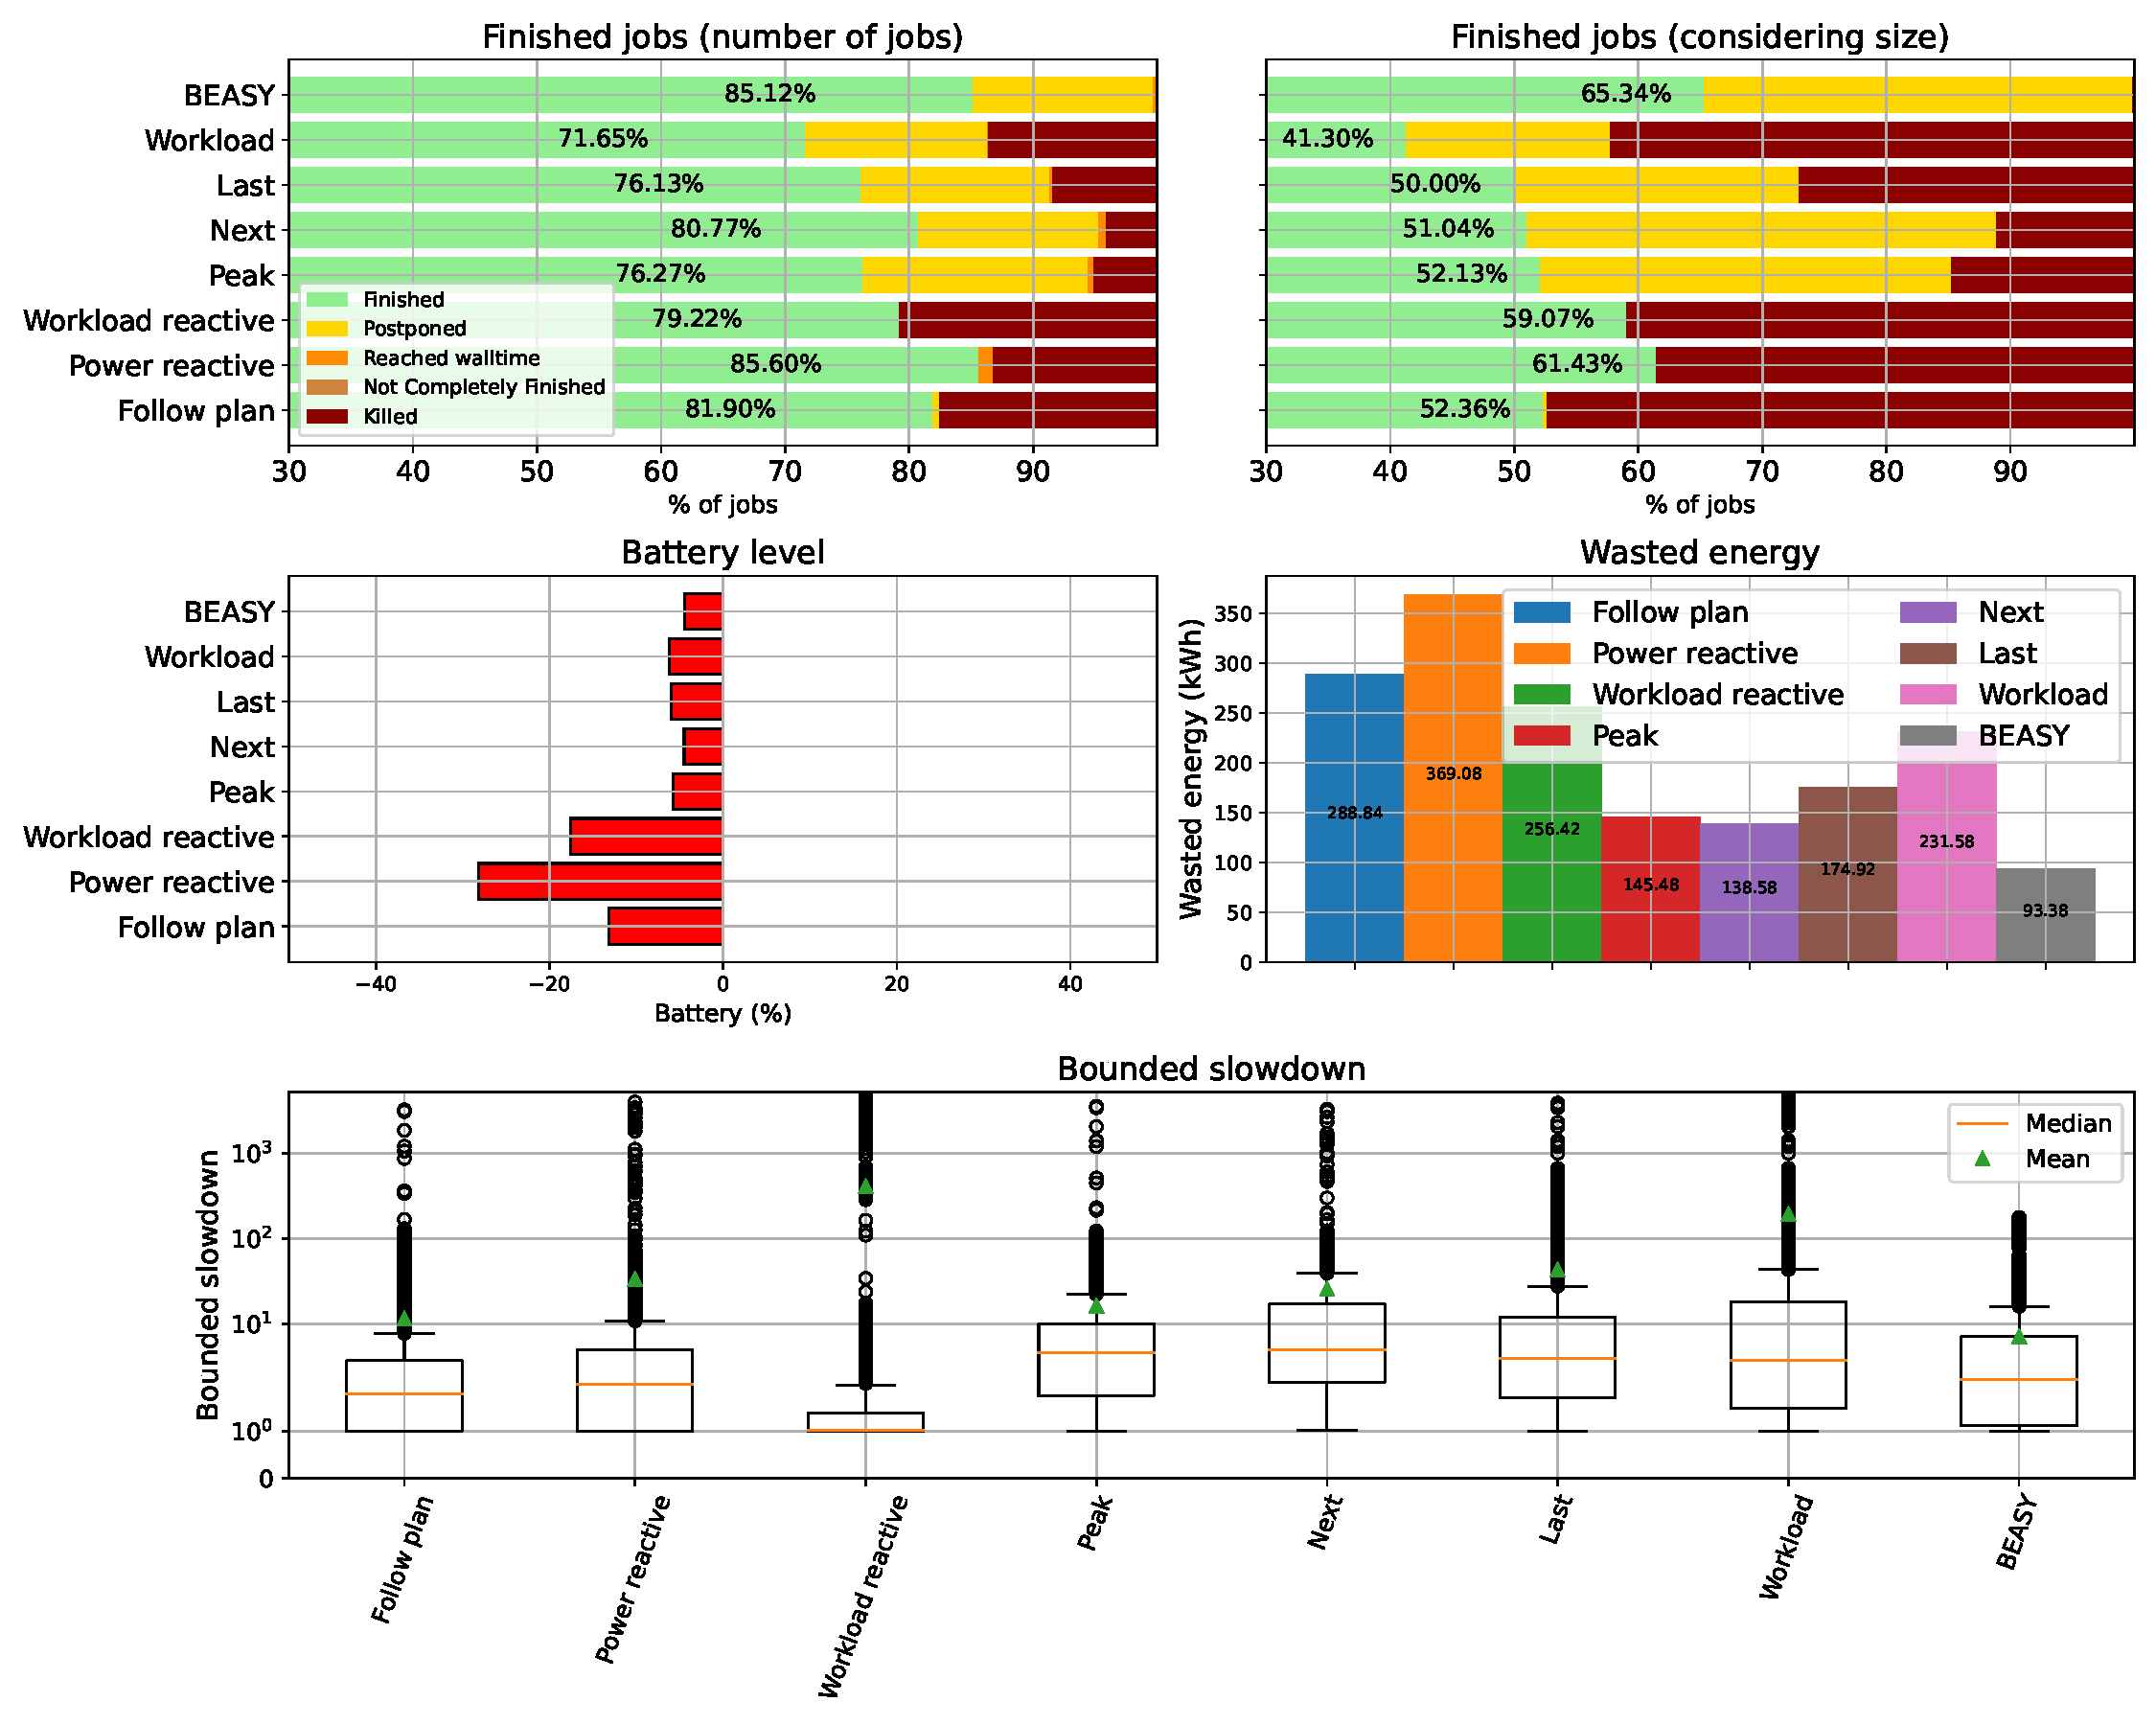
\includegraphics[scale=0.39]{Images/Heuristic/profile_worst_workload_1_with_noise.pdf}
    \caption{Results of \emph{\systemName} on critical case 3.}
    \label{fig:beasy_critical_3}
\end{figure}

\emph{\systemName} is the second best in finished jobs, very close to the best one \emph{Power reactive}. Besides, \emph{\systemName} kills very few jobs (0.10\%). Considering the size, \emph{\systemName} is the best one, finishing more than the \emph{Power reactive}. Comparing \emph{\systemName} and \emph{Power reactive}, the former has a better battery level. \emph{Power reactive} finishes with more than 20\% of battery deficit. \emph{Next} policy is the best policy, but it is worst than the \emph{\systemName} in finished jobs (in number and size). The policies and \emph{\systemName} have quite similar battery levels. \emph{\systemName} has the best result on wasted energy, reducing by 31.17\% compared to the \emph{Next} (the second-best). This is a scenario where it is essential to use energy efficiently. So this is an excellent result. Finally, \emph{\systemName} has the best mean bounded slowdown, with no job having more than 1000. The other algorithms have several jobs with a very high bounded slowdown ($>1000$). However, it has a higher median than all baselines but lower than the policies.

% \clearpage

\subsubsection{Scenario Critical 4}

The last case is with the profile worst-case and the jobs arriving at the end of the time window. Figure \ref{fig:beasy_critical_4} shows the results. 

\begin{figure}[!htb]
    \centering
    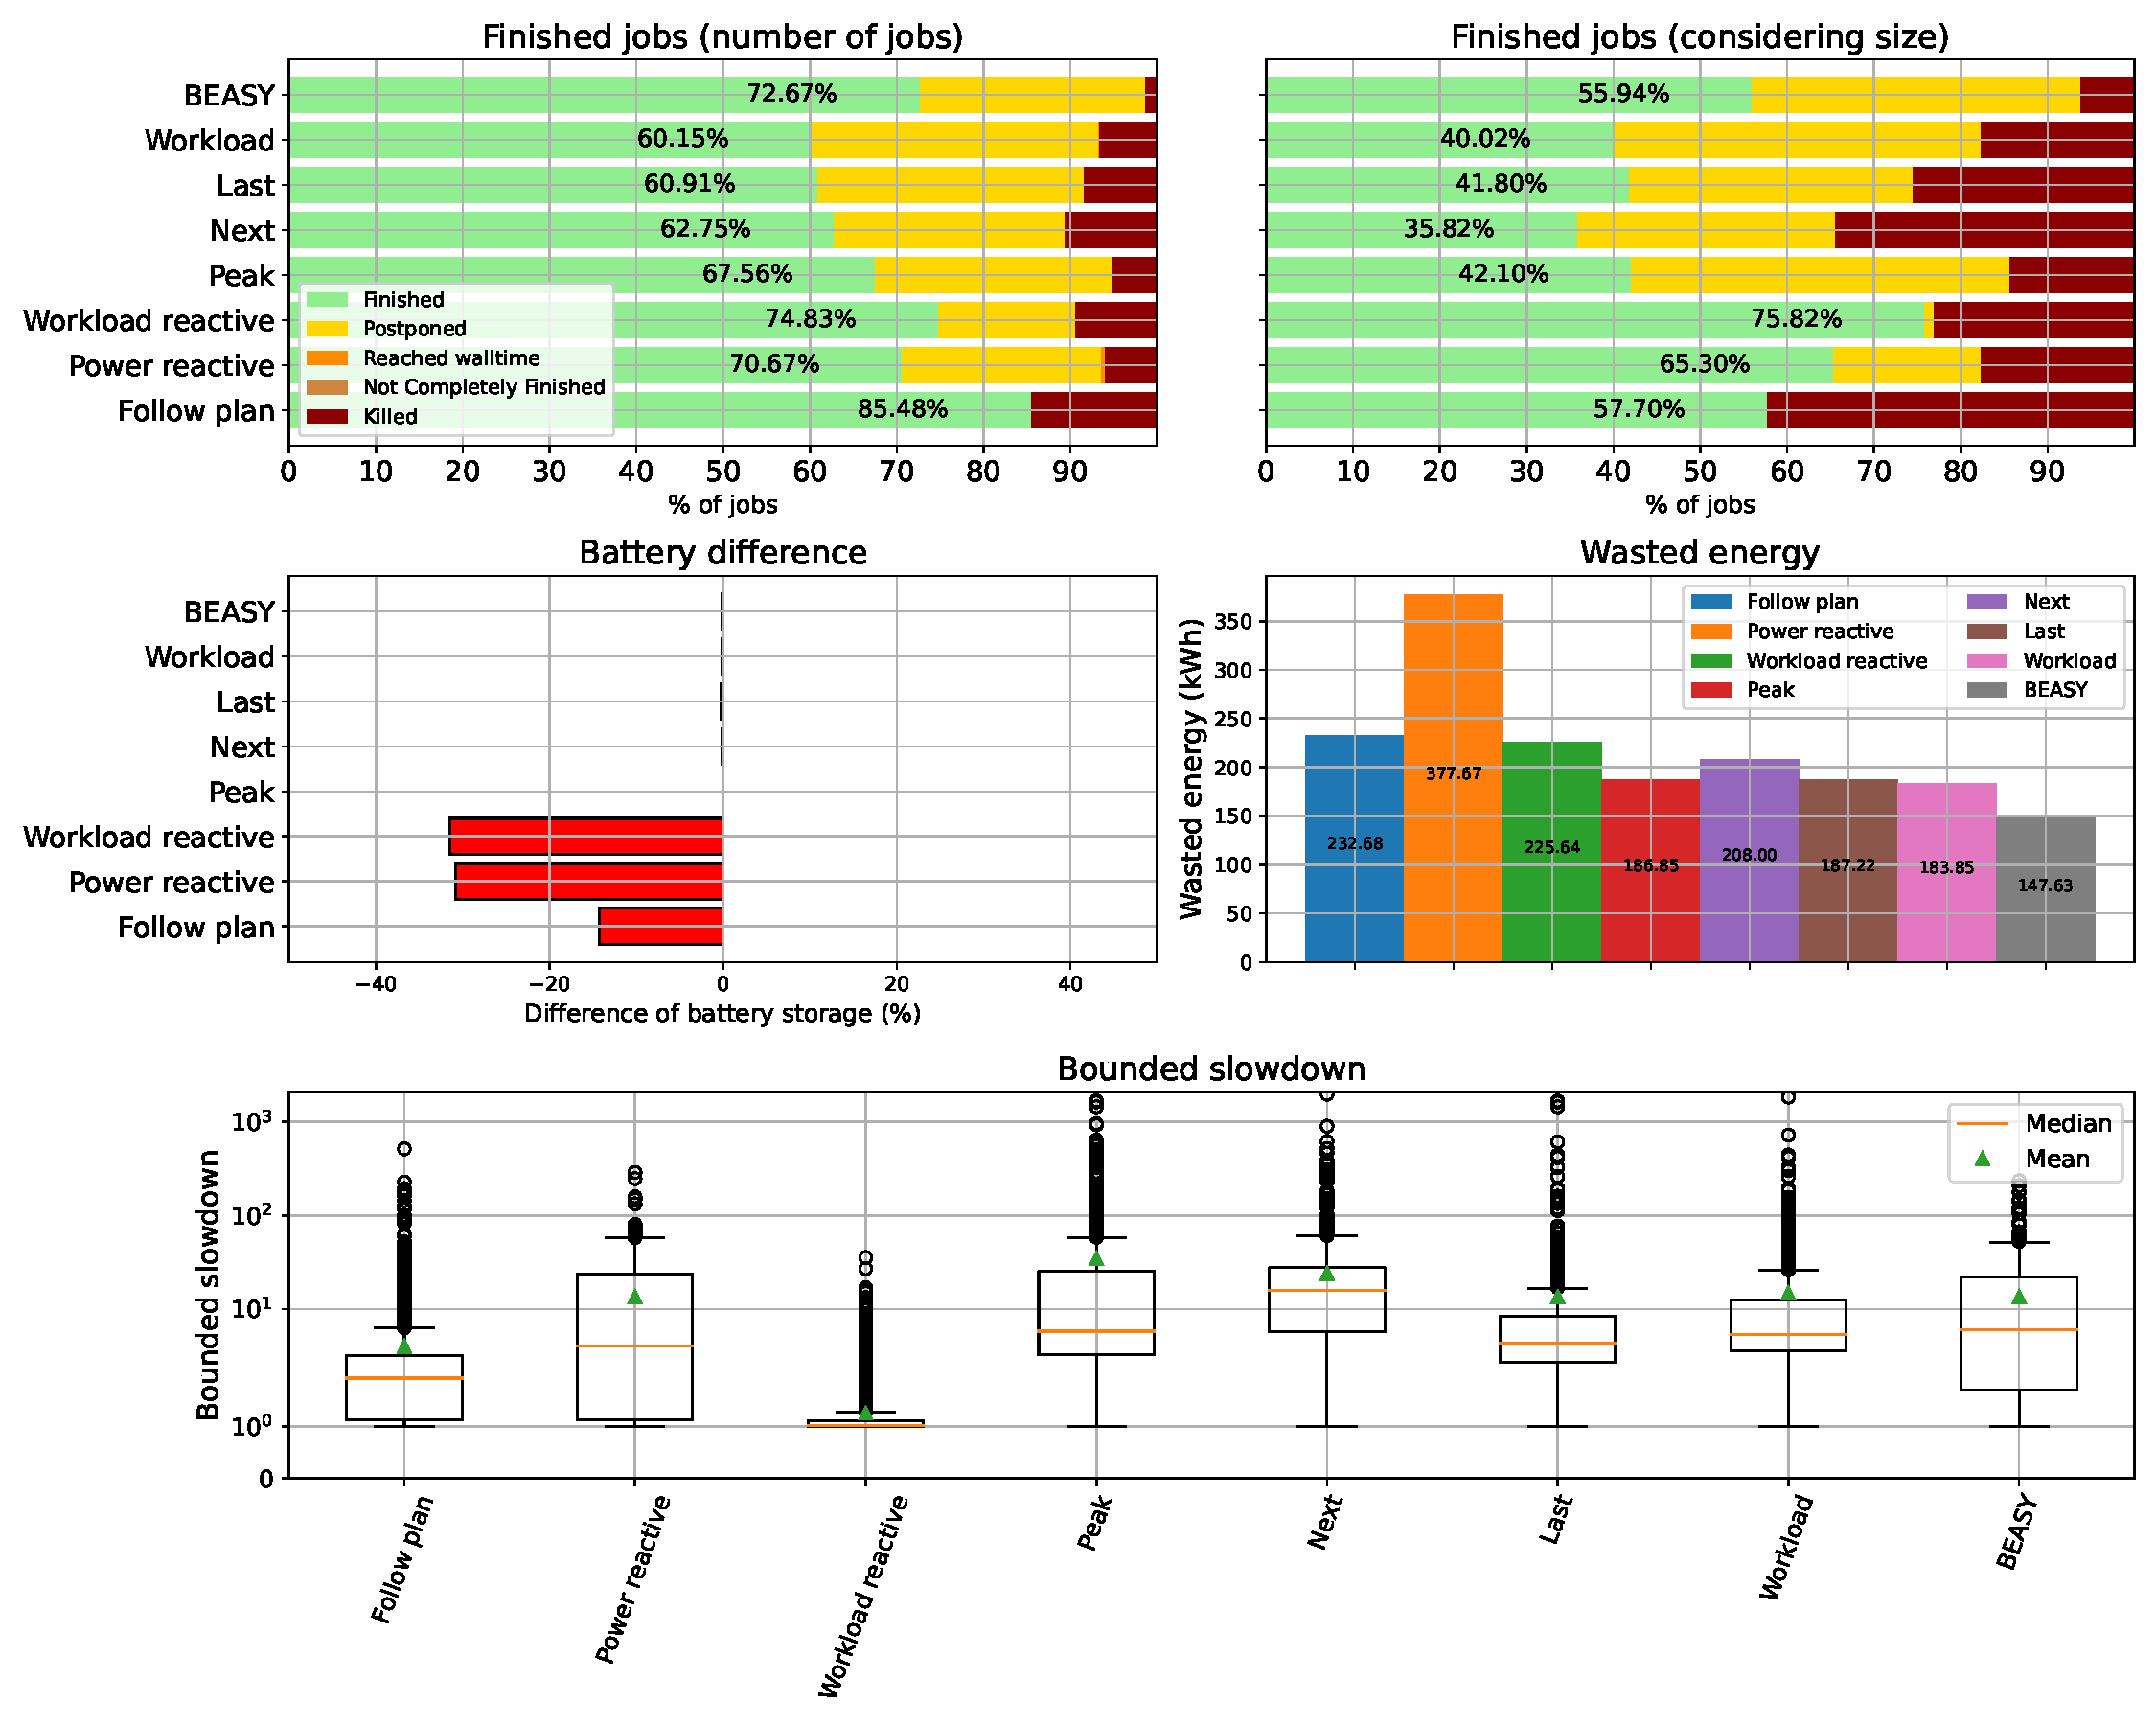
\includegraphics[scale=0.39]{Images/Heuristic/profile_worst_workload_2_with_noise.pdf}
    \caption{Results of \emph{\systemName} on critical case 4.}
    \label{fig:beasy_critical_4}
\end{figure}

Comparing \emph{\systemName} with the executions that respected the battery level (\emph{Peak}, \emph{Next}, \emph{Last}, and \emph{Workload} policies), \emph{\systemName} has the highest finished jobs (in number and sizing). Including executions that do not respect the battery level (\emph{Workload reactive}, \emph{Power reactive}, and \emph{Follow plan}), \emph{\systemName} is only better than the \emph{Power reactive} in number but finishes less in size. Besides, \emph{\systemName} finishes less than \emph{Workload reactive} and \emph{Follow plan} in number and size. However, \emph{\systemName} kills fewer jobs than all other algorithms (baselines and policies). We can see that \emph{Workload reactive} finishes in number almost the same percentage as \emph{\systemName} but finishes far from the battery target level. This scenario makes it hard to start big jobs, resulting in a big impact on the size of the jobs executed by \emph{\systemName}. Again, \emph{\systemName} has an outstanding result regarding wasted energy. It wastes less energy than all the other algorithms, with 19.70\% less than the second-best, \emph{Workload} policy. Finally, in this case, \emph{\systemName} has a higher median bounded slowdown compared to the other algorithms, but the \emph{Next} policy. The mean value of \emph{\systemName} is similar to \emph{Workload}, \emph{Last}, and \emph{Power reactive} but higher than \emph{Follow plan} and \emph{Workload reactive}. \emph{\systemName} finishes more small jobs due to the power constraints, in which the waiting time has higher importance. Since our bounded slowdown considers only the finished jobs, executing more small jobs can produce a higher slowdown.

% \clearpage

\subsection{Random cases}

After presenting the critical cases, this section details the random cases. As mentioned previously, we have taken 100 different profiles and workloads. Figure \ref{fig:beasy_average} illustrates the results of the 100 executions. 

\begin{figure}[!htb]
    \centering
    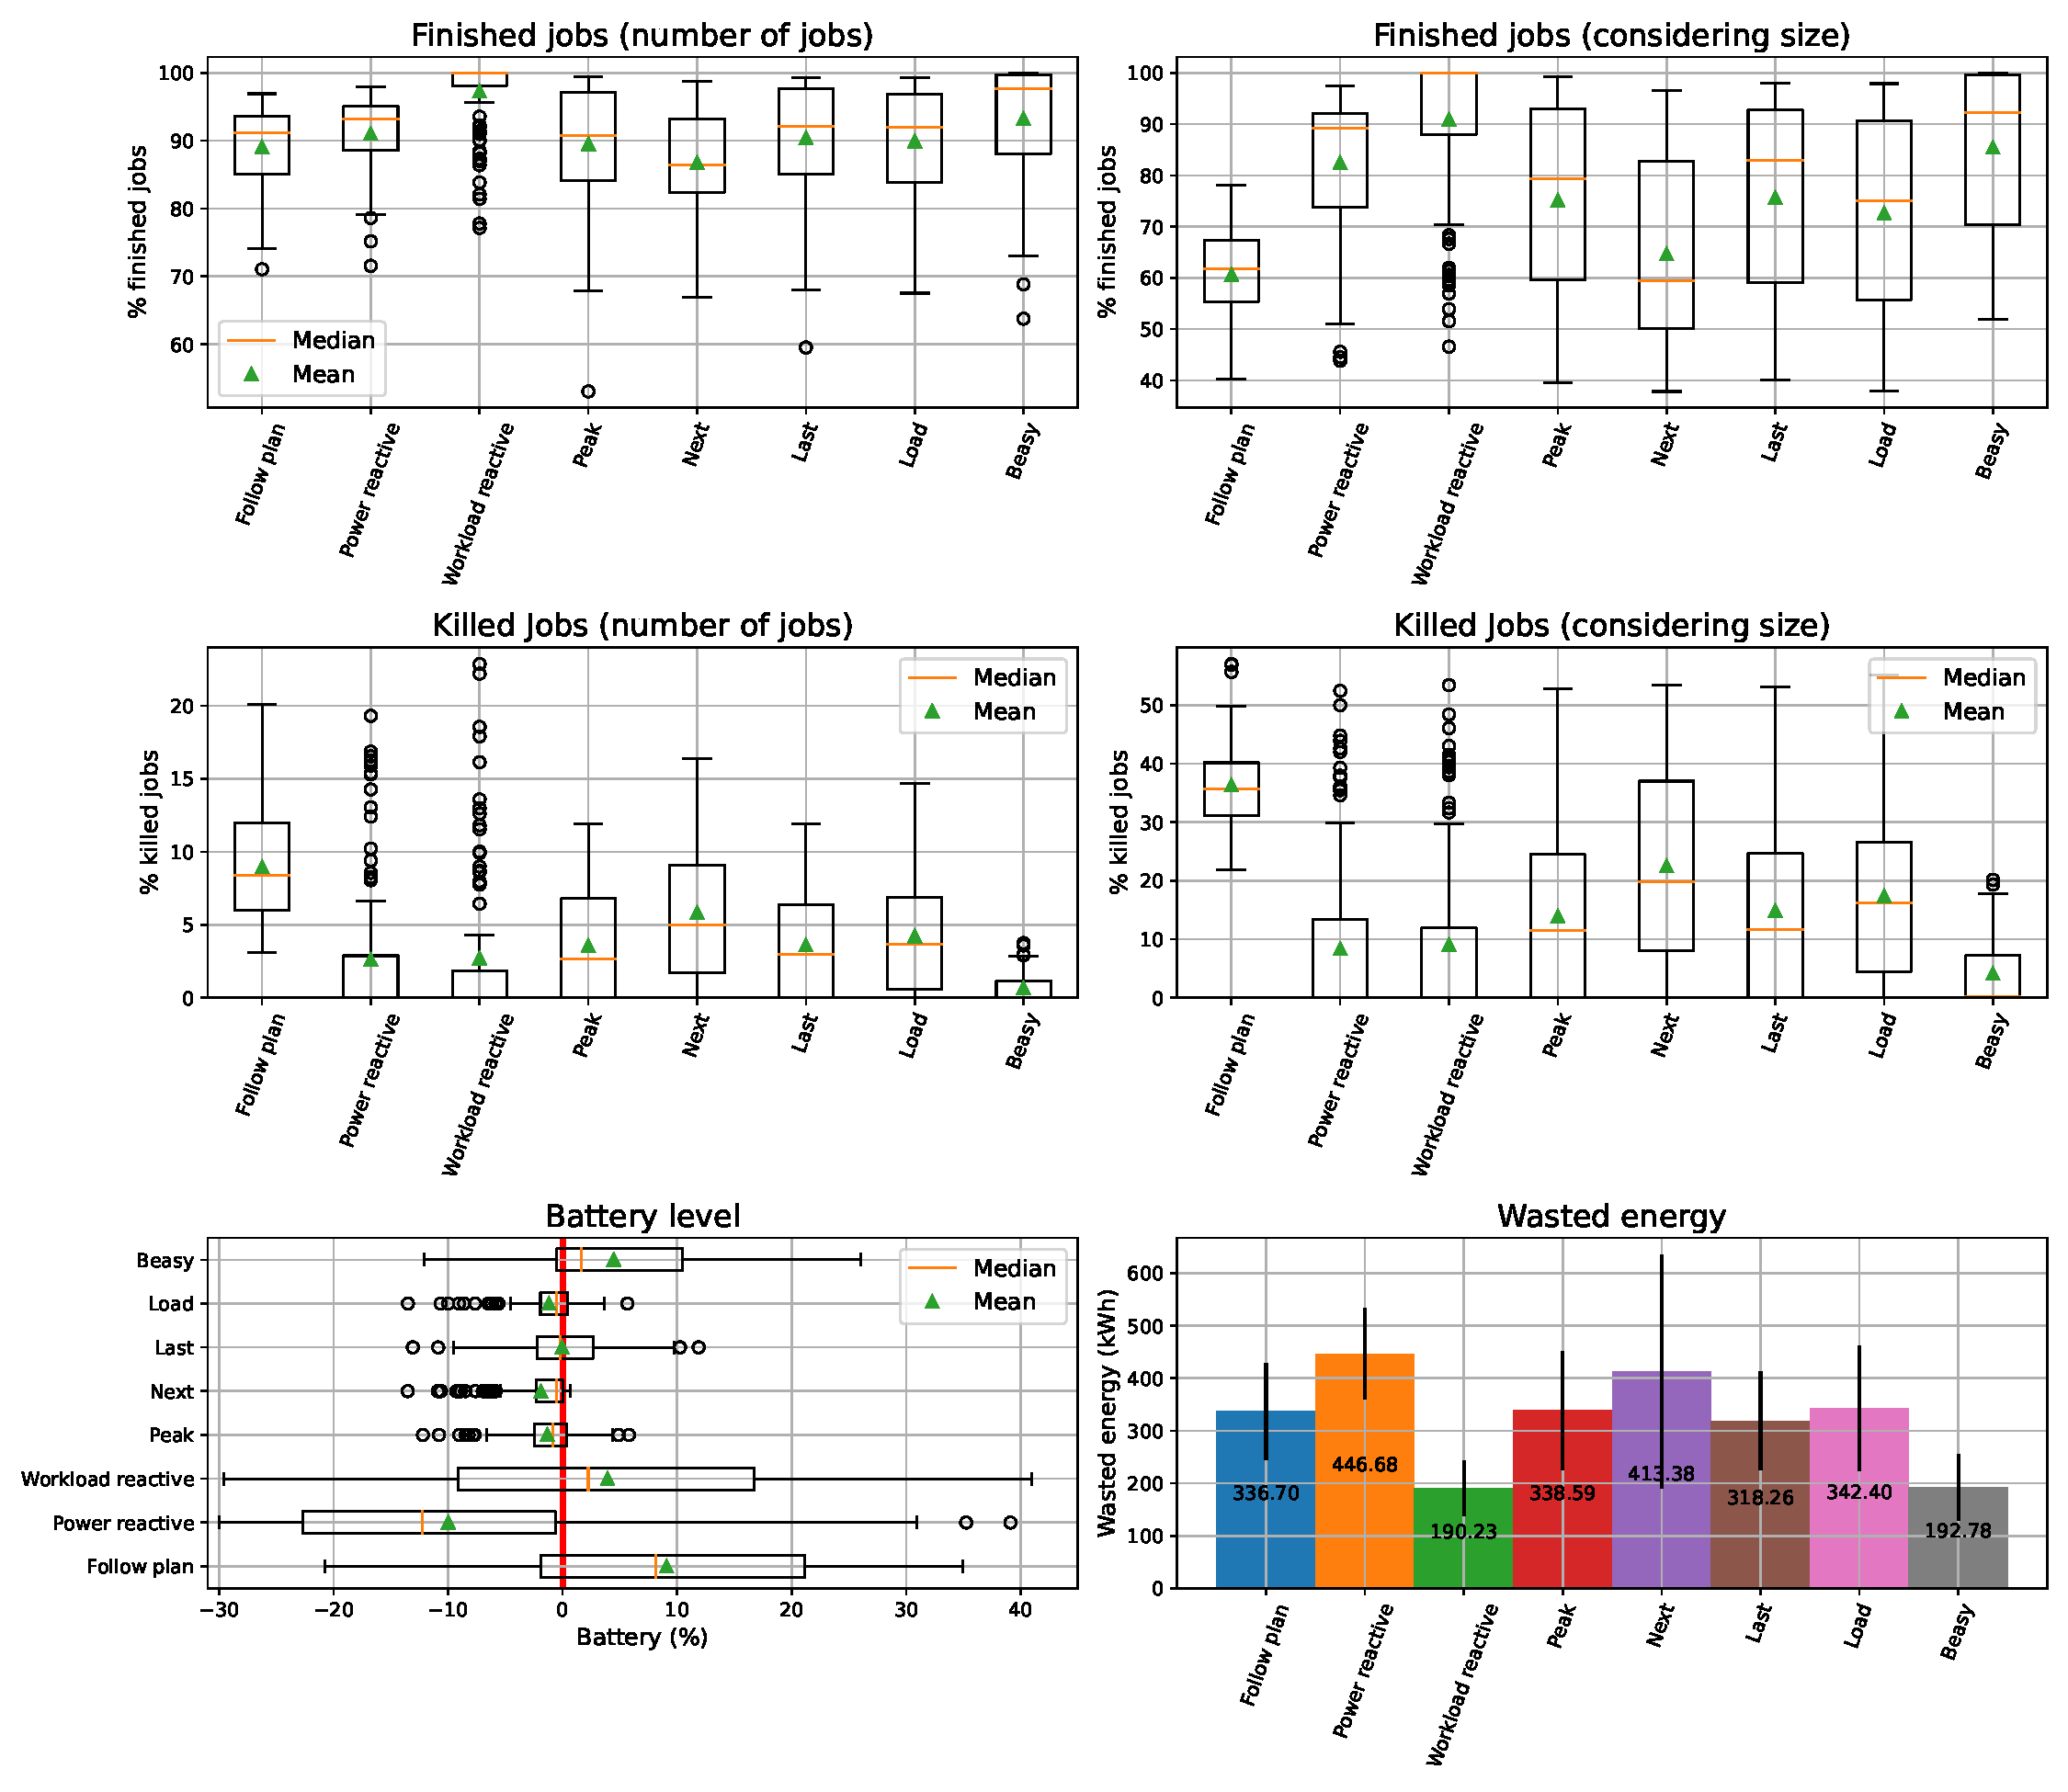
\includegraphics[scale=0.39]{Images/Heuristic/100_cases.pdf}
    \caption{Results of \emph{\systemName} on random cases.}
    \label{fig:beasy_average}
\end{figure}

Like in the critical cases, \emph{\systemName} presents the lowest number of killed jobs. \emph{\systemName} has no execution with more than 5\% (in number) or 20\% (in size) of killed jobs. The other algorithms have a higher mean and worst-case. For example, \emph{Workload reactive} has two executions with more than 20\% killed jobs in number and one execution with more than 50\% in size. The policies reduce these numbers but have higher values than \emph{\systemName}. Considering finished jobs, \emph{\systemName} has the second-best mean of 93.29\% (in number) and 85.42\% (in size). \emph{Workload reactive} has the best mean with 97.27\% (in number) and 90.86\% (in size). \emph{Workload reactive} is very aggressive, which helps to have a higher number of finished jobs but also leads to a high killed job number. Figure \ref{fig:soc_average} compares the SoC of \emph{Workload reactive} and \emph{\systemName} in the execution where \emph{Workload reactive} killed several jobs. \emph{Workload reactive} could not avoid the 20\% threshold, resulting in several killed jobs. \emph{\systemName} avoids this threshold.

\begin{figure}[!htb]
    \centering
    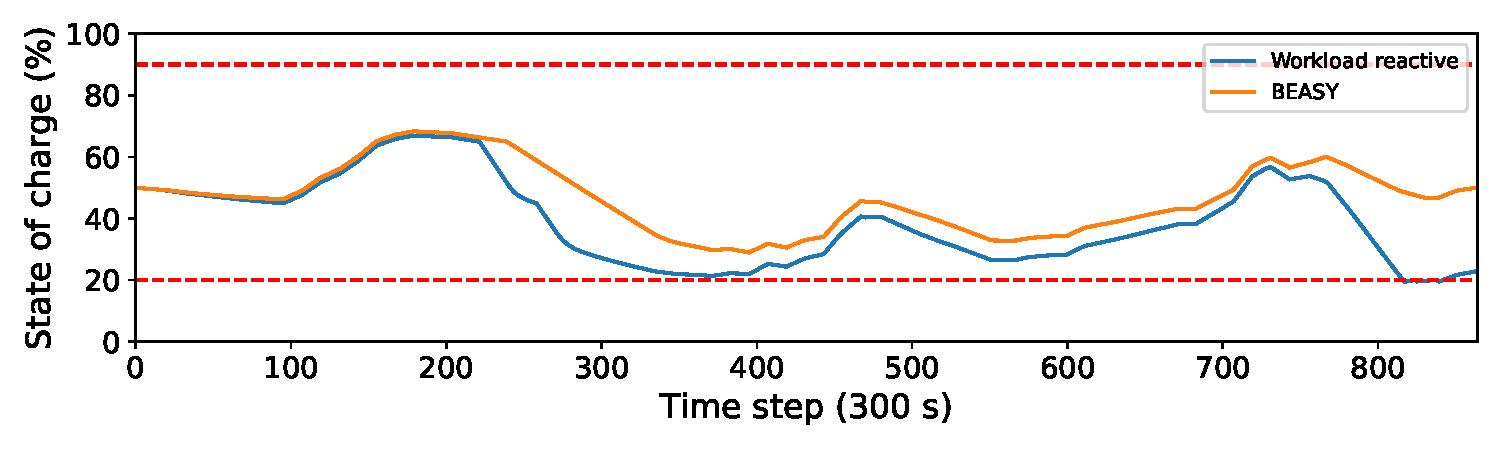
\includegraphics[scale=0.5]{Images/Heuristic/diff_state_of_charge.pdf}
    \caption[SoC comparison between \emph{Workload reactive} and \emph{\systemName}.]{SoC in one of the scenarios. \emph{Workload reactive} kills several jobs when the battery is lower than 20\%. \emph{Workload reactive} almost kills jobs between time steps 350 and 400, but it can keep SoC above 20\%. \emph{\systemName} avoids this threshold and could maintain the jobs running.}
    \label{fig:soc_average}
\end{figure}

Comparing the number of jobs killed, \emph{Workload reactive} has 19\% of the executions above 5\% of killed jobs (in number), while \emph{\systemName} has none. This result shows that \emph{\systemName} can maintain the SoC above the target level. Furthermore, \emph{Workload reactive} has the two worst number of jobs killed among all executions. \emph{Power reactive} has the third-best number of completed jobs but also 19\% of the executions above 5\% of killed jobs (in number). Considering the battery target level, \emph{\systemName} has good levels since it is near the target level (average of 54.47\%). 75\% of the executions in \emph{\systemName} finished with the battery at the target level or higher. While \emph{Workload reactive} has a wider battery level, with the minimal being close to -30\%, \emph{\systemName} has a better result. The best executions in this metric are the policies (\emph{Peak}, \emph{Next}, \emph{Last}, and \emph{Workload}), always around 50\% and with a very low standard deviation. But, we could see they can not reduce the killed jobs as much as \emph{\systemName}. Finally, \emph{\systemName} and \emph{Workload reactive} have the best result in wasted energy, well below the other executions. \emph{Workload reactive} is very energy aware since it tends to maintain running only the servers needed due to its DPM technique. So, being close to the same result is quite outstanding for \emph{\systemName}. 

\subsection{Discussion}

After presenting the results of critical and random cases, this section consolidates our discussion. Table \ref{tab:ranking} ranks all algorithms over the different tested scenarios. We highlight in green the top 3 results on each metric for each scenario. The bottom 3 results are in red. Both finished and killed jobs are considered in number. Killed jobs are: killed jobs + reach the walltime + not completely finished. For SoC, we assume the best results as the higher real SoC at the end of the time window. This table highlights the excellent results of \emph{\systemName} over the different experiments, where it finishes in top 3 in all cases. \emph{\systemName} is always the best one in killed jobs. This heuristic can identify when it is possible to execute more jobs and when it is better to be conservative, postponing some jobs. Running everything is not always possible due to power constraints in our data center environment. Postponing the jobs allows us to plan the next time window considering them. For example, the next time window could use more energy coming from hydrogen to deal with these jobs. In an online way, it is not possible to change the hydrogen usage since it has a warm-up time. Besides, offline can consider the seasonality of renewable production in its decision (e.g., spend more energy from hydrogen in winter and recharge it in summer). Even postponing jobs, \emph{\systemName} is always between the top 3 finished jobs. 

The worst result of \emph{\systemName} is third place in finished jobs in critical case 4 (Profile worst-case and workload in the end). This critical case is complicated to guarantee the execution of all jobs. The algorithm with the highest finished jobs metric (\emph{Follow plan}) also has the highest killed jobs in this scenario. Furthermore, the second-best (\emph{Workload reactive}) is the third-worst in killed jobs. On the other hand, \emph{\systemName} is the third-best in finished jobs and the best in killed jobs. \emph{Follow plan} and \emph{Workload reactive} also have worse SoC level than \emph{\systemName}. Regarding the random cases, \emph{Workload reactive} seems a good possibility. However, the third place in SoC (considering the mean) does not illustrate the variance in the SoC. Figure \ref{fig:beasy_average} shows that this algorithm varies its SoC, being very unstable. \emph{\systemName} has the second-best SoC. We can see in Figure \ref{fig:beasy_average} that \emph{\systemName} has a higher SoC variance than the policies, but it is still lower than the baselines. In addition, 75\% of its values are higher than the target level, showing that it usually finishes with more energy to use in the next time window. \emph{Follow plan} has a similar result in SoC, but this algorithm has the worst killed jobs and second-worst finished jobs. \emph{Follow plan} saves battery because it does not adapt its plan to improve QoS (finished/killed jobs). 

Besides, \emph{\systemName} also has good wasted energy over all executions. It has the best wasted energy three times and the second-best two times. The only algorithm with better results is \emph{Workload reactive}. We expected \emph{Workload reactive} to have good wasted energy since it reacts to job arrival and applies DPM to turn off the servers. Even so, \emph{\systemName} outperforms \emph{Workload reactive} in three of five scenarios. In the random cases, \emph{Workload reactive} has lower wasted energy than \emph{\systemName}, but with a very similar result. \emph{Workload reactive} has two high wasted energy results in the scenarios with lower power production due to the high number of killed jobs. Besides \emph{\systemName}, only \emph{Last} policy has no wasted energy in the bottom 3. However, \emph{Last} policy is always in third or fourth place.

Finally, let's compare \emph{\systemName} globally. \emph{\systemName} has the best overall results, showing a balanced algorithm. As mentioned before, it finishes in top 3 in all cases. \emph{Workload reactive} also has several good results, mainly regarding job metrics. However, it is too aggressive, which is not a good approach in critical cases 1 and 3 (with more jobs on the first day). On the other hand, following strictly the plan in a conservative way (\emph{Follow plan}) is not a good approach either. The proposed policies are the first step away from being too conservative, showing some good results. For example, \emph{Last} policy has only two bottom 3 QoS results in the scenarios with less energy. However, they are still not enough. \emph{\systemName} can find a balance between QoS and power constraints. The SoC predictions help the SoC to finish close to the target. The finished and killed jobs have good results in \emph{\systemName} due to its scheduling approach. The \emph{\systemName}'s scheduling validation helps to guarantee job executions. Finally, the wasted energy good results come from both scheduling and SoC predictions. Executing small jobs in dangerous moments maintains the SoC under control and reduces killed jobs. Reducing killed jobs also reduces wasted energy. So, combining good scheduling and power compensation decisions makes \emph{\systemName} achieve these outstanding results. \emph{\systemName} manages in the same way both power consumption (real-time jobs) uncertainties and power production (weather) uncertainties.

\begin{landscape}

\begin{table*}[htp]
    \centering
    \caption{Consolidate average results in every scenario.}
    \label{tab:ranking}
    \begin{tabular}{c|l||l|l|l|l|l|l|l|l}
        \hline
        Scenario                                                                                                       & Metric        & Follow plan                   & Power reactive                & Workload reactive             & Peak                          & Next                          & Last                          & Load                      & BEASY                         \\ \hline\hline
        \multirow{4}{*}{\begin{tabular}[c]{@{}c@{}}Profile best-case \\ and \\ workload in \\ beginning\end{tabular}}  & Finished jobs & {\cellcolor{red!75}}\nth{8}   & {\cellcolor{red!50}}\nth{7}   & {\cellcolor{red!25}}\nth{6}   & \nth{4}                       & \nth{5}                       & {\cellcolor{green!50}}\nth{2} & {\cellcolor{green!25}}\nth{3} & {\cellcolor{green!75}}\nth{1} \\ 
        \hhline{~---------}
                                                                                                                       & Killed jobs   & {\cellcolor{red!75}}\nth{8}   & {\cellcolor{red!50}}\nth{7}   & {\cellcolor{red!25}}\nth{6}   & \nth{4}                       & \nth{5}                       & {\cellcolor{green!50}}\nth{2} & {\cellcolor{green!25}}\nth{3} & {\cellcolor{green!75}}\nth{1} \\ \hhline{~---------}
                                                                                                                       & SoC           & {\cellcolor{green!75}}\nth{1} & {\cellcolor{red!75}}\nth{8}   & {\cellcolor{green!25}}\nth{3} & {\cellcolor{red!25}}\nth{6}   & {\cellcolor{red!50}}\nth{7}   & \nth{4}                       & \nth{5}                       & {\cellcolor{green!50}}\nth{2} \\ \hhline{~---------}
                                                                                                                       & Wasted energy & {\cellcolor{red!50}}\nth{7}   & {\cellcolor{red!75}}\nth{8}   & {\cellcolor{green!50}}\nth{2} & \nth{4}                       & {\cellcolor{red!25}}\nth{6}   & {\cellcolor{green!25}}\nth{3} & \nth{5}                       & {\cellcolor{green!75}}\nth{1} \\ \hline\hline
        \multirow{4}{*}{\begin{tabular}[c]{@{}c@{}}Profile best-case \\ and \\ workload in end\end{tabular}}           & Finished jobs & {\cellcolor{red!50}}\nth{7}   & \nth{4}                       & {\cellcolor{green!75}}\nth{1} & {\cellcolor{red!25}}\nth{6}   & {\cellcolor{red!75}}\nth{8}   & {\cellcolor{green!25}}\nth{3} & \nth{5}                       & {\cellcolor{green!50}}\nth{2} \\ \hhline{~---------}
                                                                                                                       & Killed jobs   & {\cellcolor{red!75}}\nth{8}   & \nth{5}                       & {\cellcolor{green!75}}\nth{1} & {\cellcolor{red!25}}\nth{6}   & {\cellcolor{red!50}}\nth{7}   & \nth{4}                       & {\cellcolor{green!25}}\nth{3} & {\cellcolor{green!75}}\nth{1} \\ \hhline{~---------}
                                                                                                                       & SoC           & {\cellcolor{green!75}}\nth{1} & {\cellcolor{red!75}}\nth{8}   & {\cellcolor{red!50}}\nth{7}   & {\cellcolor{green!25}}\nth{3} & \nth{4}                       & \nth{5}                       & {\cellcolor{red!25}}\nth{6}   & {\cellcolor{green!50}}\nth{2} \\ \hhline{~---------}
                                                                                                                       & Wasted energy & \nth{5}                       & {\cellcolor{red!75}}\nth{8}   & {\cellcolor{green!75}}\nth{1} & {\cellcolor{red!25}}\nth{6}   & {\cellcolor{red!50}}\nth{7}   & {\cellcolor{green!25}}\nth{3} & \nth{4}                       & {\cellcolor{green!50}}\nth{2} \\ \hline\hline
        \multirow{4}{*}{\begin{tabular}[c]{@{}c@{}}Profile worst-case \\ and \\ workload in \\ beginning\end{tabular}} & Finished jobs & {\cellcolor{green!25}}\nth{3} & {\cellcolor{green!75}}\nth{1} & \nth{5}                       & {\cellcolor{red!25}}\nth{6}   & \nth{4}                       & {\cellcolor{red!50}}\nth{7}   & {\cellcolor{red!75}}\nth{8}   & {\cellcolor{green!50}}\nth{2} \\ \hhline{~---------}
                                                                                                                       & Killed jobs   & {\cellcolor{red!50}}\nth{7}   & {\cellcolor{red!25}}\nth{6}   & {\cellcolor{red!75}}\nth{8}   & {\cellcolor{green!25}}\nth{3} & {\cellcolor{green!50}}\nth{2} & \nth{4}                       & \nth{5}                       & {\cellcolor{green!75}}\nth{1} \\ \hhline{~---------}
                                                                                                                       & SoC           & {\cellcolor{red!25}}\nth{6}   & {\cellcolor{red!75}}\nth{8}   & {\cellcolor{red!50}}\nth{7}   & {\cellcolor{green!25}}\nth{3} & {\cellcolor{green!50}}\nth{2} & \nth{4}                       & \nth{5}                       & {\cellcolor{green!75}}\nth{1} \\ \hhline{~---------}
                                                                                                                       & Wasted energy & {\cellcolor{red!50}}\nth{7}   & {\cellcolor{red!75}}\nth{8}   & {\cellcolor{red!25}}\nth{6}   & {\cellcolor{green!25}}\nth{3} & {\cellcolor{green!50}}\nth{2} & \nth{4}                       & \nth{5}                       & {\cellcolor{green!75}}\nth{1} \\ \hline\hline
        \multirow{4}{*}{\begin{tabular}[c]{@{}c@{}}Profile worst-case \\ and \\ workload in end\end{tabular}}          & Finished jobs & {\cellcolor{green!75}}\nth{1} & \nth{4}                       & {\cellcolor{green!50}}\nth{2} & \nth{5}                       & {\cellcolor{red!25}}\nth{6}   & {\cellcolor{red!50}}\nth{7}   & {\cellcolor{red!75}}\nth{8}   & {\cellcolor{green!25}}\nth{3} \\ \hhline{~---------}
                                                                                                                       & Killed jobs   & {\cellcolor{red!75}}\nth{8}   & {\cellcolor{green!25}}\nth{3} & {\cellcolor{red!25}}\nth{6}   & {\cellcolor{green!50}}\nth{2} & {\cellcolor{red!50}}\nth{7}   & \nth{5}                       & \nth{4}                       & {\cellcolor{green!75}}\nth{1} \\ \hhline{~---------}
                                                                                                                       & SoC           & {\cellcolor{red!25}}\nth{6}   & {\cellcolor{red!50}}\nth{7}   & {\cellcolor{red!75}}\nth{8}   & {\cellcolor{green!75}}\nth{1} & {\cellcolor{green!25}}\nth{3} & \nth{5}                       & \nth{4}                       & {\cellcolor{green!50}}\nth{2} \\ \hhline{~---------}
                                                                                                                       & Wasted energy & {\cellcolor{red!50}}\nth{7}   & {\cellcolor{red!75}}\nth{8}   & {\cellcolor{red!25}}\nth{6}   & {\cellcolor{green!25}}\nth{3} & \nth{5}                       & \nth{4}                       & {\cellcolor{green!50}}\nth{2} & {\cellcolor{green!75}}\nth{1} \\ \hline\hline
        \multirow{4}{*}{100 average cases}                                                                             & Finished jobs & {\cellcolor{red!50}}\nth{7}   & {\cellcolor{green!25}}\nth{3} & {\cellcolor{green!75}}\nth{1} & {\cellcolor{red!25}}\nth{6}   & {\cellcolor{red!75}}\nth{8}   & \nth{4}                       & \nth{5}                       & {\cellcolor{green!50}}\nth{2} \\ \hhline{~---------}
                                                                                                                       & Killed jobs   & {\cellcolor{red!75}}\nth{8}   & {\cellcolor{red!25}}\nth{6}   & {\cellcolor{green!50}}\nth{2} & \nth{4}                       & {\cellcolor{red!50}}\nth{7}   & {\cellcolor{green!25}}\nth{3} & \nth{5}                       & {\cellcolor{green!75}}\nth{1} \\ \hhline{~---------}
                                                                                                                       & SoC           & {\cellcolor{green!75}}\nth{1} & {\cellcolor{red!75}}\nth{8}   & {\cellcolor{green!25}}\nth{3} & {\cellcolor{red!25}}\nth{6}   & {\cellcolor{red!50}}\nth{7}   & \nth{4}                       & \nth{5}                       & {\cellcolor{green!50}}\nth{2} \\ \hhline{~---------}
                                                                                                                       & Wasted energy & \nth{4}                       & {\cellcolor{red!75}}\nth{8}   & {\cellcolor{green!75}}\nth{1} & \nth{5}                       & {\cellcolor{red!50}}\nth{7}   & {\cellcolor{green!25}}\nth{3} & {\cellcolor{red!25}}\nth{6}   & {\cellcolor{green!50}}\nth{2} \\ \hline
    \end{tabular}
\end{table*}

\end{landscape}

\section{Conclusion}

This chapter presented and evaluated \emph{\systemName}, a heuristic that mixes power and scheduling decisions. \emph{\systemName} uses power production and demand predictions to estimate the SoC. This SoC estimation helps to make better power compensation decisions. Besides, \emph{\systemName} identifies dangerous moments where the SoC could be too close to the battery's lower boundary. In these dangerous moments, \emph{\systemName} starts to be conservative, preferring to run small over big jobs. On the scheduling side, it validates if the job can run entirely. It verifies if the job's servers are available during the entire execution or if it is possible to migrate energy to maintain the servers running. We compared \emph{\systemName} with three baselines (\emph{Follow plan}, \emph{Power reactive}, and \emph{Workload reactive}) and the four policies presented in Chapter \ref{cha:power_compensations}. \emph{\systemName} showed outstanding results in finished jobs, killed jobs, SoC difference from the target, and wasted energy. It is in the top 3 of all metrics in every scenario. We could see that \emph{\systemName} manages the different objectives of QoS and energy storage.
    
    \chapter{Conclusion and Perspectives}
\label{cha:conclusion}

In this chapter, we make overall conclusions and summarize the contributions of this work, along with a discussion of future work.

\section{Conclusion}

The world has a big challenge to reduce its GHG emissions and stop global warming. GHG reduction demands the engagement of all sectors of governments, industry, and research. One sector is Information and Communication Technology (ICT) with emissions in 2020 around 1.8\%-2.8\% or 2.1\%-3.9\% considering the supply chain pathways. Data centers are one of the actors inside ICT with a good share of the emissions. Both academy and industries focus their efforts on reducing emissions of the big data center providers. Reducing their emissions is particularly difficult due to the growth in Internet users and network devices. Even with this growth, the emissions did not increase at the same pace due mainly to the power optimizations. However, some authors claim that these power consumption improvements are close to their limit. Therefore, data center providers must find other ways to reduce emissions, such as renewable energy migration.

Some providers, such as Google and Amazon, are investing in an off-site renewable production approach to maintain their servers. In an off-site generation, the data center and power production are not in the same place. So, the providers generate the same amount of energy to the grid that they expend on their servers. However, the biggest challenge of renewable sources is the power intermittence. Since RES production comes from nature, it depends on the climate conditions. Therefore, these providers transfer the problem to third parties. In a net zero scenario (where no energy comes from brown sources), they can not maintain their quality of service without changing the strategy. 

The Datazero2 project proposes an architecture and decision process for a renewable-only data center. The architecture is disconnected from the power grid, using only the energy produced by solar panels and wind turbines but with power storage as backups. Using just renewable sources demand different decision levels. We divided the decision level into two possibilities: offline and online. The offline approach has time to search for an optimal solution to match power production and demand. Usually, it predicts both production and demand. The main drawback of the offline approach is that it does not know the real events, so its optimal solution only works if the predictions are good enough. On the other hand, the online approach reacts to real events. However, an online-only approach is myopic, ignoring long-term decisions. In this thesis, we proposed ways to mix offline and online dealing with uncertainties from power production and consumption. We demonstrated in Chapter \ref{cha:related_work} a lack of propositions mixing both. The main objectives of an integrated offline-online approach are to improve the QoS (maximizing finished jobs and reducing killed jobs), respect the power constraints (approximating battery target level), and reduce the wasted energy (maximizing renewable usage).

First, we focused on respecting the power constraints. So, we proposed four compensation policies to adapt power usage, approximating the battery target level at the end of the time window. The compensation changes the power usage according to the power fluctuations derived from production/consumption variations. The compensation policies are \emph{Peak}, \emph{Last}, \emph{Next}, and \emph{Workload}. All policies arrive with better battery levels than the baselines (\emph{Follow plan}, \emph{Power reactive}, and \emph{Workload reactive}). The policies improved the finished jobs in the scenarios with more energy available, compared to an offline-only execution (\emph{Follow plan}). In scenarios with less energy available, they reduced the number of finished jobs but approximated the target battery level at the end of the time window. Nevertheless, there was not a good policy in every execution, demanding further improvements.

The second contribution tried to introduce a Reinforcement Learning (RL) model to make better compensation decisions. Since every policy arrived at a good battery level at the end of the time window, we tried to mix the compensations driven by a QoS metric. Therefore, we proposed an RL model with two reward propositions linked to QoS (finished and started jobs). The idea is still to compensate for power variations, which proved to be enough to respect the power constraint, but choosing the actions which improved QoS. We proposed two RL algorithms: Q-Learning and Contextual Multi-Armed Bandit with LinUCB. The results show that they could not improve the QoS, resulting in even worse QoS. These results were explained by several factors, such as chained decisions making it harder to find the best actions, the reward did not represent the global QoS, state/action size limitations, and separated scheduling and power decisions.

Finally, the last contribution is a heuristic which consolidates all the aspects discovered in previous sections. The heuristic is named \emph{\systemName} and englobes the compensation idea (from the policies) and solves the problems from the Reinforcement Learning, such as mixing scheduling and power decisions and using more information from the state of charge estimation. Besides, this heuristic is completely parameterizable, in size aspects (number of servers, power production, battery sizes, etc.) and constraints (SoC target level, SoC boundaries, etc.). We compared \emph{\systemName} with the baselines and policies, showing good overall results of the new heuristic. \emph{\systemName} had the lowest killed jobs than all the other algorithms while respecting the power constraints. Regarding the finished jobs, it was among the top-3 in every scenario. \emph{Workload reactive} maintains the servers sleeping until a job arrives. This behavior helps this algorithm to have low wasted energy. Even so, \emph{\systemName} had lower wasted energy than \emph{Workload reactive} in three of five cases. 

\section{Perspectives}

The work presented in this thesis proposes some ways to mix offline and online decisions in a renewable-only data center. As perspectives, there are some remaining subjects for further improvement.

\textbf{Change learning process}
% Other RL algorithms
% Deep RL

As we presented in Chapter \ref{cha:learning_power_compensations}, our model for learning the best compensations did not improve the policy's results. We presented several problems in our model. Therefore, future work can introduce a different learning algorithm, such as Deep Reinforcement Learning (DRL). DRL allows a larger state and action space. Using a larger state space, we could introduce more variables, such as jobs waiting to run, estimated SoC of the future steps (time series), the actual state of running jobs, etc. Besides, the action space can be more precise, using the right step to compensate. Future work can compare DRL with the heuristics in the time and energy spent to learn and apply the algorithms. Another possibility is changing our reward for the total finished and killed jobs of a time window. This reward demands more learning iterations in a simple RL but could produce better results. We hypothesized that doing the best local actions would result in the best global results. However, we saw that this is not true. 

\textbf{Add flexibility in energy constraints}
% Add a \% of flexibility in the target level
% Use hydrogen

The model presented in Chapter \ref{cha:model} considered a hard constraint of the battery's SoC at the end of the time window. Even if the algorithms (policies and \emph{\systemName}) did not finish with the exact target level, their decisions consider this battery constraint. Future work can evaluate the possibility of a flexible battery level. For example, they can accept $\pm 5\%$ as flexibility at the end of the time window. This flexibility can improve even more the QoS, running more jobs and reducing killed jobs. However, this flexibility must be studied along with the PDM module. Giving $\pm 5\%$ as the battery's flexibility would finish the battery with $-5\%$ than the target in every scenario (the algorithms use all the possible energy available). Nevertheless, this behavior can lead to PDM demanding an overestimated target level (e.g., always $+5\%$), which does not change the actual behavior. Another possibility is to introduce hydrogen decisions in the model. In the current model, we considered hydrogen production as fixed input production without changes due to the hydrogen's slow dynamics. However, the online model can consider hydrogen dynamics and use hydrogen in critical cases, following recent and future developments in Hydrogen technologies. As for the battery's flexibility, this must be studied together with PDM.

\textbf{Modify the application type}
% Services in general
% Streaming

This thesis focused on batch applications. Future work can evaluate \emph{\systemName} and the policies for other application types. For example, let's imagine a renewable-only streaming scheduler using \emph{\systemName}. A new user sends a request to watch a video from the catalog. The catalog has several videos with different sizes. The video size can be our walltime, which \emph{\systemName} uses to estimate the energy demanded. The user should wait for his time to watch (supposing that they agreed with this to use clean energy). Changing the processor's speed would impact the video quality. Killing a job interrupts the streaming. In dangerous moments (SoC close to the battery lower boundary), \emph{\systemName} lets only small videos. We can evaluate the QoS (waiting time, quality degradation, etc) of \emph{\systemName} in this environment. A possible uncertainty comes from the possibility of pausing the video, which changes the video's finish time. Another possible future work is to introduce in the model other job aspects, such as memory, network communication, etc. This thesis considered that the jobs are impacted only by the CPU. Even if this is the main factor, it is not the only one. Besides, we can evaluate the impact of killed jobs resubmission.

\textbf{Explore different time definitions}
% time window
% time step
% chained time windows

Our work considered a time window of three days and a time step of five minutes. The time window size is not too long to make it difficult to predict the weather conditions and not too short to reduce ODM decision possibilities. In addition, the time step is short enough to maintain ODM reactive (e.g., fastly adapt battery usage) and long enough to finish the server transitions (e.g., the server on and off). However, future works can compare different time windows and time steps, to find the best configurations. For example, would a time window of one day impact the ODM decisions? And a time window of one week? Does a longer time step be too late to adapt power usage? Another possible evaluation is to evaluate chained time windows. For example, the execution of Datazero2 during one year with all modules integrated. This thesis created some offline modules without a direct connection with the online. We ran the offline optimizations, generating input for the online experiments. A complete one-year execution demands the total Datazero2 middleware implementation. 

\textbf{Miscellaneous data centers}

Our experiments focused on a data center with on-site renewable power production. We considered only the servers in our power consumption. However, more complex architecture can include network consumption, cooling, etc. A new version of \emph{\systemName} could consider the impact of these additional elements in decision-making. In the first approach, we could consider the power consumption of these elements constant, and just introduce them in the power consumption model. However, are they constant? How can we introduce the cooling in the scheduling decision? Another possibility is to introduce \emph{\systemName} in a distributed data center. This kind of data center can maximize renewable usage even more, by following the production by the sun. In the first moment, \emph{\systemName} can be applied individually in each site. However, is it sufficient? Is a new decision level (such as the site to place a job definition) necessary? How does \emph{\systemName} need to manage the battery (globally or locally)?



    \bibliographystyle{unsrtnat}
    \bibliography{library}

\end{document}
